
%подсказки по LaTeX http://mydebianblog.blogspot.ru/2008/11/latex.html] 
\documentclass[a4paper,14pt]{extreport}

%\documentclass[a4paper,14pt]{report} %размер бумаги устанавливаем А4, шрифт 12пунктов
\renewcommand{\baselinestretch}{1.5} %1,5 междустрочный интервал
\usepackage{ucs} %Зачем этот пакет, если уже utf подключен 

%%Перенес по причине не работы русского текста в математическом режиме
\usepackage{xcolor}	%цветовые настройки гиперссылок
\usepackage{hyperref} %генерация гиперссылок
% Цвета для гиперссылок
\definecolor{linkcolor}{HTML}{799B03} % цвет ссылок
\definecolor{urlcolor}{HTML}{799B03} % цвет гиперссылок
\hypersetup{pdfstartview=FitH,  linkcolor=linkcolor,urlcolor=urlcolor, colorlinks=true}
%Русские символы в математическом режиме
%\usepackage[warn]{mathtext}   
\usepackage{mathtext}   
\usepackage[T2A]{fontenc}
\usepackage[utf8x]{inputenc} % Включаем поддержку UTF8
%\usepackage{times} % Шрифт Times New Roman
\usepackage[small]{titlesec} % чуть уменьшаем размер заголовков глав и разделов
\usepackage[english, russian]{babel}%используем русский и английский языки с переносами

%%Работа с математическими пакетами
\usepackage{amsmath}
\usepackage{mathtools}

%Для вида (2.1.1)
\numberwithin{equation}{section}
%%Понятия зачем это
\newcommand\normalsubformula[1]{\text{\mathversion{normal}$#1$}}

\usepackage{amsfonts}
\usepackage{amssymb}
\usepackage{cite}
\usepackage{enumerate}
\usepackage{float}

\usepackage{indentfirst} %Включаем первый отступ для абзаца
\usepackage{geometry} % Меняем поля страницы
	\geometry{left=2cm}% левое поле
	\geometry{right=1.5cm}% правое поле
	\geometry{top=1cm}% верхнее поле
	\geometry{bottom=2cm}% нижнее поле

\usepackage[final]{graphicx}
\graphicspath{{images/}}%путь к рисункам
\RequirePackage{caption}
	\DeclareCaptionLabelSeparator{defffis}{ -- }
	\captionsetup{justification=centering,labelsep=defffis}
	\renewcommand{\theenumi}{\arabic{enumi}}% Меняем везде перечисления на цифра.цифра
	\renewcommand{\labelenumi}{\arabic{enumi}}% Меняем везде перечисления на цифра.цифра
	\renewcommand{\theenumii}{.\arabic{enumii}}% Меняем везде перечисления на цифра.цифра
	\renewcommand{\labelenumii}{\arabic{enumi}.\arabic{enumii}.}% Меняем везде перечисления на цифра.цифра
	\renewcommand{\theenumiii}{.\arabic{enumiii}}% Меняем везде перечисления на цифра.цифра
	\renewcommand{\labelenumiii}{\arabic{enumi}.\arabic{enumii}.\arabic{enumiii}.}% Меняем везде перечисления на цифра.цифра




%%%%%Что-бы Latex не плевался ошибками на время 
% List styles
\newcounter{saveenum}
\newcommand\liststyleWWviiiNumxiii{%
	\renewcommand\theenumi{\arabic{enumi}}
	\renewcommand\theenumii{\arabic{enumii}}
	\renewcommand\theenumiii{\arabic{enumiii}}
	\renewcommand\labelitemi{}
	\renewcommand\labelenumi{\theenumi.}
	\renewcommand\labelenumii{\theenumii.}
	\renewcommand\labelenumiii{\theenumiii.}
}
\newcommand\liststyleWWviiiNumxvii{%
	\renewcommand\theenumi{\arabic{enumi}}
	\renewcommand\theenumii{\arabic{enumii}}
	\renewcommand\theenumiii{\arabic{enumiii}}
	\renewcommand\labelitemi{}
	\renewcommand\labelenumi{\theenumi.}
	\renewcommand\labelenumii{\theenumii.}
	\renewcommand\labelenumiii{\theenumiii.}
}
\newcommand\liststyleWWviiiNumxxi{%
	\renewcommand\theenumi{\arabic{enumi}}
	\renewcommand\theenumii{\arabic{enumii}}
	\renewcommand\theenumiii{\arabic{enumiii}}
	\renewcommand\labelitemi{}
	\renewcommand\labelenumi{\theenumi.}
	\renewcommand\labelenumii{\theenumii.}
	\renewcommand\labelenumiii{\theenumiii.}
}
\newcommand\liststyleWWviiiNumvii{%
	\renewcommand\theenumi{\arabic{enumi}}
	\renewcommand\theenumii{\arabic{enumii}}
	\renewcommand\theenumiii{\arabic{enumiii}}
	\renewcommand\labelitemi{}
	\renewcommand\labelenumi{\theenumi.}
	\renewcommand\labelenumii{\theenumii.}
	\renewcommand\labelenumiii{\theenumiii.}
}
\newcommand\liststyleWWviiiNumlxxiii{%
	\renewcommand\theenumi{\arabic{enumi}}
	\renewcommand\theenumii{\arabic{enumii}}
	\renewcommand\theenumiii{\arabic{enumiii}}
	\renewcommand\labelitemi{}
	\renewcommand\labelenumi{\theenumi.}
	\renewcommand\labelenumii{\theenumii.}
	\renewcommand\labelenumiii{\theenumiii.}
}
\newcommand\liststyleWWviiiNumli{%
	\renewcommand\theenumi{\arabic{enumi}}
	\renewcommand\theenumii{\arabic{enumii}}
	\renewcommand\theenumiii{\arabic{enumiii}}
	\renewcommand\labelitemi{}
	\renewcommand\labelenumi{\theenumi.}
	\renewcommand\labelenumii{\theenumii.}
	\renewcommand\labelenumiii{\theenumiii.}
}
\newcommand\liststyleWWviiiNumxxvii{%
	\renewcommand\theenumi{\arabic{enumi}}
	\renewcommand\theenumii{\arabic{enumii}}
	\renewcommand\theenumiii{\arabic{enumiii}}
	\renewcommand\theenumiv{\arabic{enumiv}}
	\renewcommand\labelenumi{\theenumi).}
	\renewcommand\labelenumii{\theenumii.}
	\renewcommand\labelenumiii{\theenumiii.}
	\renewcommand\labelenumiv{\theenumiv.}
}
\newcommand\liststyleWWviiiNumlxviii{%
	\renewcommand\theenumi{\arabic{enumi}}
	\renewcommand\theenumii{\arabic{enumii}}
	\renewcommand\theenumiii{\arabic{enumiii}}
	\renewcommand\theenumiv{\arabic{enumiv}}
	\renewcommand\labelenumi{\theenumi).}
	\renewcommand\labelenumii{\theenumii.}
	\renewcommand\labelenumiii{\theenumiii.}
	\renewcommand\labelenumiv{\theenumiv.}
}
\newcommand\liststyleWWviiiNumlxxiv{%
	\renewcommand\theenumi{\arabic{enumi}}
	\renewcommand\theenumii{\arabic{enumii}}
	\renewcommand\theenumiii{\arabic{enumiii}}
	\renewcommand\labelitemi{}
	\renewcommand\labelenumi{\theenumi.}
	\renewcommand\labelenumii{\theenumii.}
	\renewcommand\labelenumiii{\theenumiii.}
}
\newcommand\liststyleWWviiiNumi{%
	\renewcommand\theenumi{\arabic{enumi}}
	\renewcommand\theenumii{\arabic{enumii}}
	\renewcommand\theenumiii{\arabic{enumiii}}
	\renewcommand\theenumiv{\arabic{enumiv}}
	\renewcommand\labelenumi{\theenumi)}
	\renewcommand\labelenumii{\theenumii.}
	\renewcommand\labelenumiii{\theenumiii.}
	\renewcommand\labelenumiv{\theenumiv.}
}
\newcommand\liststyleWWviiiNumx{%
	\renewcommand\theenumi{\arabic{enumi}}
	\renewcommand\theenumii{\arabic{enumii}}
	\renewcommand\theenumiii{\arabic{enumiii}}
	\renewcommand\labelitemi{}
	\renewcommand\labelenumi{\theenumi.}
	\renewcommand\labelenumii{\theenumii.}
	\renewcommand\labelenumiii{\theenumiii.}
}
\newcommand\liststyleWWviiiNumxxxix{%
	\renewcommand\theenumi{\arabic{enumi}}
	\renewcommand\theenumii{\arabic{enumii}}
	\renewcommand\theenumiii{\arabic{enumiii}}
	\renewcommand\labelitemi{}
	\renewcommand\labelenumi{\theenumi.}
	\renewcommand\labelenumii{\theenumii.}
	\renewcommand\labelenumiii{\theenumiii.}
}
\newcommand\liststyleWWviiiNumxlviii{%
	\renewcommand\theenumi{\arabic{enumi}}
	\renewcommand\theenumii{\arabic{enumii}}
	\renewcommand\theenumiii{\arabic{enumiii}}
	\renewcommand\labelitemi{}
	\renewcommand\labelenumi{\theenumi.}
	\renewcommand\labelenumii{\theenumii.}
	\renewcommand\labelenumiii{\theenumiii.}
}
\newcommand\liststyleWWviiiNumxlvi{%
	\renewcommand\theenumi{\arabic{enumi}}
	\renewcommand\theenumii{\arabic{enumii}}
	\renewcommand\theenumiii{\arabic{enumiii}}
	\renewcommand\labelitemi{}
	\renewcommand\labelenumi{\theenumi.}
	\renewcommand\labelenumii{\theenumii.}
	\renewcommand\labelenumiii{\theenumiii.}
}
\newcommand\liststyleWWviiiNumxv{%
	\renewcommand\theenumi{\arabic{enumi}}
	\renewcommand\theenumii{\arabic{enumii}}
	\renewcommand\theenumiii{\arabic{enumiii}}
	\renewcommand\labelitemi{}
	\renewcommand\labelenumi{\theenumi.}
	\renewcommand\labelenumii{\theenumii.}
	\renewcommand\labelenumiii{\theenumiii.}
}
\newcommand\liststyleWWviiiNumlxxvii{%
	\renewcommand\theenumi{\arabic{enumi}}
	\renewcommand\theenumii{\arabic{enumii}}
	\renewcommand\theenumiii{\arabic{enumiii}}
	\renewcommand\labelitemi{}
	\renewcommand\labelenumi{\theenumi.}
	\renewcommand\labelenumii{\theenumii.}
	\renewcommand\labelenumiii{\theenumiii.}
}
\newcommand\liststyleWWviiiNumxlii{%
	\renewcommand\theenumi{\arabic{enumi}}
	\renewcommand\theenumii{\arabic{enumii}}
	\renewcommand\theenumiii{\arabic{enumiii}}
	\renewcommand\labelitemi{}
	\renewcommand\labelenumi{\theenumi.}
	\renewcommand\labelenumii{\theenumii.}
	\renewcommand\labelenumiii{\theenumiii.}
}
\newcommand\liststyleWWviiiNumlxxi{%
	\renewcommand\theenumi{\arabic{enumi}}
	\renewcommand\theenumii{\arabic{enumii}}
	\renewcommand\theenumiii{\arabic{enumiii}}
	\renewcommand\labelitemi{}
	\renewcommand\labelenumi{\theenumi.}
	\renewcommand\labelenumii{\theenumii.}
	\renewcommand\labelenumiii{\theenumiii.}
}
\newcommand\liststyleWWviiiNumlxix{%
	\renewcommand\theenumi{\arabic{enumi}}
	\renewcommand\theenumii{\arabic{enumii}}
	\renewcommand\theenumiii{\arabic{enumiii}}
	\renewcommand\labelitemi{}
	\renewcommand\labelenumi{\theenumi.}
	\renewcommand\labelenumii{\theenumii.}
	\renewcommand\labelenumiii{\theenumiii.}
}
\newcommand\liststyleWWviiiNumlxxviii{%
	\renewcommand\theenumi{\arabic{enumi}}
	\renewcommand\theenumii{\arabic{enumii}}
	\renewcommand\theenumiii{\arabic{enumiii}}
	\renewcommand\labelitemi{}
	\renewcommand\labelenumi{\theenumi.}
	\renewcommand\labelenumii{\theenumii.}
	\renewcommand\labelenumiii{\theenumiii.}
}
\newcommand\liststyleWWviiiNumxxxvii{%
	\renewcommand\theenumi{\arabic{enumi}}
	\renewcommand\theenumii{\arabic{enumii}}
	\renewcommand\theenumiii{\arabic{enumiii}}
	\renewcommand\labelitemi{}
	\renewcommand\labelenumi{\theenumi.}
	\renewcommand\labelenumii{\theenumii.}
	\renewcommand\labelenumiii{\theenumiii.}
}
\newcommand\liststyleWWviiiNumviii{%
	\renewcommand\theenumi{\arabic{enumi}}
	\renewcommand\theenumii{\arabic{enumii}}
	\renewcommand\theenumiii{\arabic{enumiii}}
	\renewcommand\labelitemi{}
	\renewcommand\labelenumi{\theenumi.}
	\renewcommand\labelenumii{\theenumii.}
	\renewcommand\labelenumiii{\theenumiii.}
}
\newcommand\liststyleWWviiiNumlii{%
	\renewcommand\theenumi{\arabic{enumi}}
	\renewcommand\theenumii{\arabic{enumii}}
	\renewcommand\theenumiii{\arabic{enumiii}}
	\renewcommand\theenumiv{\arabic{enumiv}}
	\renewcommand\labelenumi{\theenumi)}
	\renewcommand\labelenumii{\theenumii.}
	\renewcommand\labelenumiii{\theenumiii.}
	\renewcommand\labelenumiv{\theenumiv.}
}
\newcommand\liststyleWWviiiNumxxv{%
	\renewcommand\theenumi{\arabic{enumi}}
	\renewcommand\theenumii{\arabic{enumii}}
	\renewcommand\theenumiii{\arabic{enumiii}}
	\renewcommand\theenumiv{\arabic{enumiv}}
	\renewcommand\labelenumi{\theenumi.}
	\renewcommand\labelenumii{\theenumii.}
	\renewcommand\labelenumiii{\theenumiii.}
	\renewcommand\labelenumiv{\theenumiv.}
}
\newcommand\liststyleWWviiiNumlxxii{%
	\renewcommand\theenumi{\arabic{enumi}}
	\renewcommand\theenumii{\arabic{enumii}}
	\renewcommand\theenumiii{\arabic{enumiii}}
	\renewcommand\theenumiv{\arabic{enumiv}}
	\renewcommand\labelenumi{\theenumi)}
	\renewcommand\labelenumii{\theenumii.}
	\renewcommand\labelenumiii{\theenumiii.}
	\renewcommand\labelenumiv{\theenumiv.}
}
\newcommand\liststyleWWviiiNumlxx{%
	\renewcommand\theenumi{\arabic{enumi}}
	\renewcommand\theenumii{\arabic{enumii}}
	\renewcommand\theenumiii{\arabic{enumiii}}
	\renewcommand\theenumiv{\arabic{enumiv}}
	\renewcommand\labelenumi{\theenumi).}
	\renewcommand\labelenumii{\theenumii.}
	\renewcommand\labelenumiii{\theenumiii.}
	\renewcommand\labelenumiv{\theenumiv.}
}
\newcommand\liststyleWWviiiNumxxxiv{%
	\renewcommand\theenumi{\arabic{enumi}}
	\renewcommand\theenumii{\arabic{enumii}}
	\renewcommand\theenumiii{\arabic{enumiii}}
	\renewcommand\theenumiv{\arabic{enumiv}}
	\renewcommand\labelenumi{\theenumi)}
	\renewcommand\labelenumii{\theenumii.}
	\renewcommand\labelenumiii{\theenumiii.}
	\renewcommand\labelenumiv{\theenumiv.}
}
\newcommand\liststyleWWviiiNumlxvi{%
	\renewcommand\theenumi{\arabic{enumi}}
	\renewcommand\theenumii{\arabic{enumii}}
	\renewcommand\theenumiii{\arabic{enumiii}}
	\renewcommand\theenumiv{\arabic{enumiv}}
	\renewcommand\labelenumi{\theenumi.}
	\renewcommand\labelenumii{\theenumii.}
	\renewcommand\labelenumiii{\theenumiii.}
	\renewcommand\labelenumiv{\theenumiv.}
}
\newcommand\liststyleWWviiiNumliii{%
	\renewcommand\theenumi{\arabic{enumi}}
	\renewcommand\theenumii{\arabic{enumii}}
	\renewcommand\theenumiii{\arabic{enumiii}}
	\renewcommand\labelitemi{}
	\renewcommand\labelenumi{\theenumi.}
	\renewcommand\labelenumii{\theenumii.}
	\renewcommand\labelenumiii{\theenumiii.}
}
\newcommand\liststyleWWviiiNumliv{%
	\renewcommand\theenumi{\arabic{enumi}}
	\renewcommand\theenumii{\arabic{enumii}}
	\renewcommand\theenumiii{\arabic{enumiii}}
	\renewcommand\labelitemi{}
	\renewcommand\labelenumi{\theenumi.}
	\renewcommand\labelenumii{\theenumii.}
	\renewcommand\labelenumiii{\theenumiii.}
}
\newcommand\liststyleWWviiiNumxxxvi{%
	\renewcommand\theenumi{\arabic{enumi}}
	\renewcommand\theenumii{\arabic{enumii}}
	\renewcommand\theenumiii{\arabic{enumiii}}
	\renewcommand\labelitemi{}
	\renewcommand\labelenumi{\theenumi.}
	\renewcommand\labelenumii{\theenumii.}
	\renewcommand\labelenumiii{\theenumiii.}
}
\newcommand\liststyleWWviiiNumxlv{%
	\renewcommand\theenumi{\arabic{enumi}}
	\renewcommand\theenumii{\arabic{enumii}}
	\renewcommand\theenumiii{\arabic{enumiii}}
	\renewcommand\theenumiv{\arabic{enumiv}}
	\renewcommand\labelenumi{\theenumi.}
	\renewcommand\labelenumii{\theenumii.}
	\renewcommand\labelenumiii{\theenumiii.}
	\renewcommand\labelenumiv{\theenumiv.}
}
\newcommand\liststyleWWviiiNumlxxx{%
	\renewcommand\theenumi{\arabic{enumi}}
	\renewcommand\theenumii{\arabic{enumii}}
	\renewcommand\theenumiii{\arabic{enumiii}}
	\renewcommand\theenumiv{\arabic{enumiv}}
	\renewcommand\labelenumi{\theenumi.}
	\renewcommand\labelenumii{\theenumii.}
	\renewcommand\labelenumiii{\theenumiii.}
	\renewcommand\labelenumiv{\theenumiv.}
}
\newcommand\liststyleWWviiiNumxlvii{%
	\renewcommand\theenumi{\arabic{enumi}}
	\renewcommand\theenumii{\arabic{enumii}}
	\renewcommand\theenumiii{\arabic{enumiii}}
	\renewcommand\labelitemi{}
	\renewcommand\labelenumi{\theenumi.}
	\renewcommand\labelenumii{\theenumii.}
	\renewcommand\labelenumiii{\theenumiii.}
}
\newcommand\liststyleWWviiiNumxiv{%
	\renewcommand\theenumi{\arabic{enumi}}
	\renewcommand\theenumii{\arabic{enumii}}
	\renewcommand\theenumiii{\arabic{enumiii}}
	\renewcommand\labelitemi{}
	\renewcommand\labelenumi{\theenumi.}
	\renewcommand\labelenumii{\theenumii.}
	\renewcommand\labelenumiii{\theenumiii.}
}
\newcommand\liststyleWWviiiNumxxxi{%
	\renewcommand\theenumi{\arabic{enumi}}
	\renewcommand\theenumii{\arabic{enumii}}
	\renewcommand\theenumiii{\arabic{enumiii}}
	\renewcommand\theenumiv{\arabic{enumiv}}
	\renewcommand\labelenumi{\theenumi.}
	\renewcommand\labelenumii{\theenumii.}
	\renewcommand\labelenumiii{\theenumiii.}
	\renewcommand\labelenumiv{\theenumiv.}
}
\newcommand\liststyleWWviiiNumxxii{%
	\renewcommand\theenumi{\arabic{enumi}}
	\renewcommand\theenumii{\arabic{enumii}}
	\renewcommand\theenumiii{\arabic{enumiii}}
	\renewcommand\theenumiv{\arabic{enumiv}}
	\renewcommand\labelenumi{\theenumi.}
	\renewcommand\labelenumii{\theenumii.}
	\renewcommand\labelenumiii{\theenumiii.}
	\renewcommand\labelenumiv{\theenumiv.}
}
\newcommand\liststyleWWviiiNumlxxv{%
	\renewcommand\theenumi{\arabic{enumi}}
	\renewcommand\theenumii{\arabic{enumii}}
	\renewcommand\theenumiii{\arabic{enumiii}}
	\renewcommand\theenumiv{\arabic{enumiv}}
	\renewcommand\labelenumi{\theenumi.}
	\renewcommand\labelenumii{\theenumii.}
	\renewcommand\labelenumiii{\theenumiii.}
	\renewcommand\labelenumiv{\theenumiv.}
}
\newcommand\liststyleWWviiiNumxi{%
	\renewcommand\theenumi{\arabic{enumi}}
	\renewcommand\theenumii{\alph{enumii}}
	\renewcommand\theenumiii{\roman{enumiii}}
	\renewcommand\theenumiv{\arabic{enumiv}}
	\renewcommand\labelenumi{\theenumi.}
	\renewcommand\labelenumii{\theenumii.}
	\renewcommand\labelenumiii{\theenumiii.}
	\renewcommand\labelenumiv{\theenumiv.}
}
\newcommand\liststyleWWviiiNumlxxix{%
	\renewcommand\theenumi{\arabic{enumi}}
	\renewcommand\theenumii{\arabic{enumii}}
	\renewcommand\theenumiii{\arabic{enumiii}}
	\renewcommand\theenumiv{\arabic{enumiv}}
	\renewcommand\labelenumi{\theenumi.}
	\renewcommand\labelenumii{\theenumii.}
	\renewcommand\labelenumiii{\theenumiii.}
	\renewcommand\labelenumiv{\theenumiv.}
}
\newcommand\liststyleWWviiiNumxxvi{%
	\renewcommand\theenumi{\arabic{enumi}}
	\renewcommand\theenumii{\arabic{enumii}}
	\renewcommand\theenumiii{\arabic{enumiii}}
	\renewcommand\theenumiv{\arabic{enumiv}}
	\renewcommand\labelenumi{\theenumi.}
	\renewcommand\labelenumii{\theenumii.}
	\renewcommand\labelenumiii{\theenumiii.}
	\renewcommand\labelenumiv{\theenumiv.}
}
\newcommand\liststyleWWviiiNumxxix{%
	\renewcommand\theenumi{\arabic{enumi}}
	\renewcommand\theenumii{\arabic{enumii}}
	\renewcommand\theenumiii{\arabic{enumiii}}
	\renewcommand\theenumiv{\arabic{enumiv}}
	\renewcommand\labelenumi{\theenumi.}
	\renewcommand\labelenumii{\theenumii.}
	\renewcommand\labelenumiii{\theenumiii.}
	\renewcommand\labelenumiv{\theenumiv.}
}
\newcommand\liststyleWWviiiNumxliii{%
	\renewcommand\theenumi{\arabic{enumi}}
	\renewcommand\theenumii{\arabic{enumii}}
	\renewcommand\theenumiii{\arabic{enumiii}}
	\renewcommand\theenumiv{\arabic{enumiv}}
	\renewcommand\labelenumi{\theenumi.}
	\renewcommand\labelenumii{\theenumii.}
	\renewcommand\labelenumiii{\theenumiii.}
	\renewcommand\labelenumiv{\theenumiv.}
}
\newcommand\liststyleWWviiiNumlix{%
	\renewcommand\theenumi{\arabic{enumi}}
	\renewcommand\theenumii{\arabic{enumii}}
	\renewcommand\theenumiii{\arabic{enumiii}}
	\renewcommand\theenumiv{\arabic{enumiv}}
	\renewcommand\labelenumi{\theenumi.}
	\renewcommand\labelenumii{\theenumii.}
	\renewcommand\labelenumiii{\theenumiii.}
	\renewcommand\labelenumiv{\theenumiv.}
}
\newcommand\liststyleWWviiiNumxxx{%
	\renewcommand\theenumi{\arabic{enumi}}
	\renewcommand\theenumii{\arabic{enumii}}
	\renewcommand\theenumiii{\arabic{enumiii}}
	\renewcommand\theenumiv{\arabic{enumiv}}
	\renewcommand\labelenumi{\theenumi.}
	\renewcommand\labelenumii{\theenumii.}
	\renewcommand\labelenumiii{\theenumiii.}
	\renewcommand\labelenumiv{\theenumiv.}
}
\newcommand\liststyleWWviiiNumxvi{%
	\renewcommand\theenumi{\Roman{enumi}}
	\renewcommand\theenumii{\alph{enumii}}
	\renewcommand\theenumiii{\roman{enumiii}}
	\renewcommand\theenumiv{\arabic{enumiv}}
	\renewcommand\labelenumi{\theenumi.}
	\renewcommand\labelenumii{\theenumii.}
	\renewcommand\labelenumiii{\theenumiii.}
	\renewcommand\labelenumiv{\theenumiv.}
}
\newcommand\liststyleWWviiiNumlxxvi{%
	\renewcommand\theenumi{\arabic{enumi}}
	\renewcommand\theenumii{\alph{enumii}}
	\renewcommand\theenumiii{\roman{enumiii}}
	\renewcommand\theenumiv{\arabic{enumiv}}
	\renewcommand\labelenumi{\theenumi.}
	\renewcommand\labelenumii{\theenumii.}
	\renewcommand\labelenumiii{\theenumiii.}
	\renewcommand\labelenumiv{\theenumiv.}
}
\newcommand\liststyleWWviiiNumix{%
	\renewcommand\theenumi{\arabic{enumi}}
	\renewcommand\theenumii{\alph{enumii}}
	\renewcommand\theenumiii{\roman{enumiii}}
	\renewcommand\theenumiv{\arabic{enumiv}}
	\renewcommand\labelenumi{\theenumi.}
	\renewcommand\labelenumii{\theenumii.}
	\renewcommand\labelenumiii{\theenumiii.}
	\renewcommand\labelenumiv{\theenumiv.}
}
\newcommand\liststyleWWviiiNumlxvii{%
	\renewcommand\theenumi{\arabic{enumi}}
	\renewcommand\theenumii{\alph{enumii}}
	\renewcommand\theenumiii{\roman{enumiii}}
	\renewcommand\theenumiv{\arabic{enumiv}}
	\renewcommand\labelenumi{\theenumi.}
	\renewcommand\labelenumii{\theenumii.}
	\renewcommand\labelenumiii{\theenumiii.}
	\renewcommand\labelenumiv{\theenumiv.}
}
\newcommand\liststyleWWviiiNuml{%
	\renewcommand\theenumi{\Roman{enumi}}
	\renewcommand\theenumii{\arabic{enumii}}
	\renewcommand\theenumiii{\roman{enumiii}}
	\renewcommand\theenumiv{\arabic{enumiv}}
	\renewcommand\labelenumi{\theenumi.}
	\renewcommand\labelenumii{\theenumii.}
	\renewcommand\labelenumiii{\theenumiii.}
	\renewcommand\labelenumiv{\theenumiv.}
}
\newcommand\liststyleWWviiiNumxxxviii{%
	\renewcommand\theenumi{\arabic{enumi}}
	\renewcommand\theenumii{\alph{enumii}}
	\renewcommand\theenumiii{\roman{enumiii}}
	\renewcommand\theenumiv{\arabic{enumiv}}
	\renewcommand\labelenumi{\theenumi.}
	\renewcommand\labelenumii{\theenumii.}
	\renewcommand\labelenumiii{\theenumiii.}
	\renewcommand\labelenumiv{\theenumiv.}
}
\newcommand\liststyleWWviiiNumlxi{%
	\renewcommand\theenumi{\arabic{enumi}}
	\renewcommand\theenumii{\alph{enumii}}
	\renewcommand\theenumiii{\roman{enumiii}}
	\renewcommand\theenumiv{\arabic{enumiv}}
	\renewcommand\labelenumi{\theenumi.}
	\renewcommand\labelenumii{\theenumii.}
	\renewcommand\labelenumiii{\theenumiii.}
	\renewcommand\labelenumiv{\theenumiv.}
}
%\input{prelambXetex}
%opening
\title{
	ОСНОВЫ ТЕОРИИ
	АВТОМАТИЧЕСКОГО
	УПРАВЛЕНИЯ
	}
\date{2016}

\begin{document}
	\maketitle
	\tableofcontents % это оглавление, которое генерируется автоматически
	\newpage
	\chapter{Тест}
\section{Введение в теорию автоматического управления}
На рубеже XVIII-XIX веков в эпоху промышленного переворота в Европе начинается новый этап развития автоматики, связанный с внедрением ее в промышленность. 1765 год знаменуется постройкой регулятора уровня котла паровой машины И.И. Ползунова. В 1784 го-ду появляется центробежный регулятор скорости паровой машины Дж.Уатта.

В это время формируется ряд важных принципов автоматики: принцип регулирования по отклонению Ползунова - Уатта и принцип регулирования по нагрузке Понселе. Первый из них развился в концепцию обратной связи, второй - в теорию инвариантности (Г.В. Щи-панов, Н.Н. Лузин, Б.Н. Петров). Идея регулирования по нагрузке может быть проиллюстрирована на примере генератора с последова-тельным (сериесным) возбуждением (рис.~\ref{fig:regpovozmusheniu}). При изменении нагрузки меняется ток возбуждения, который соответствующим изменением магнитного потока компенсирует дополнительное падение напряжения на внутреннем сопротивлении якоря генератора. Однако если при этом по каким-либо причинам изменяется скорость вращения якоря генератора, то застабилизировать напряжение на нагрузке в этой схеме уже не удается.

\begin{figure}[h]
	\centering
	\includegraphics[scale=0.95]{images/RegPoVozmusheniu}
	\caption{Пример регулирования по возмущению }
	\label{fig:regpovozmusheniu}
\end{figure}

От этого недостатка свободна схема, приведенная на рис.~\ref{fig:stabilizaciyanapryazenia} - именно вследствие использования принципа обратной связи. В этой схеме входной потенциометр служит для задания (коэффициент ) величины стабилизируемого напряжения; потенциометр, подключенный к якорю генератора, позволяет регулировать коэффициент об-ратной связи . В этом случае, в отличие от систем регулирования по возмущению, не важно, какая именно причина вызвала изменение регулируемой величины. При изменении напряжения на щётках генератора в соответствии с электрической схемой изменяется напряжение на обмотке возбуждения. При отрицательном знаке обратной связи знак приращения напряжения возбуждения противоположен знаку изменения напряжения якоря генератора. В итоге результирующая величина отклонения напряжения генератора уменьшается по сравнению с соответствующим уходом напряжения в системе без обратной связи. 

\begin{figure}[h]
	\centering
	\includegraphics[scale=0.95]{images/StabilizaciyaNapryazenia}
	\caption{Стабилизация напряжения генератора с использованием обратной связи}
	\label{fig:stabilizaciyanapryazenia}
\end{figure}

На этом же принципе построена приведенная на рис.~\ref{fig:steammashine} система стабилизации скорости паровой машины Уатта. На рис.\ref{fig:functionstabilization} представ-лена её функциональная схема. В данной системе с увеличением нагрузочного момента $ M_{Н} $ падают обороты турбины $ \omega $, что приводит к уменьшению расстояния $ 2r $между грузиками центробежного регулятора. Вследствие этого заслонка поднимается (увеличивается расстояние $ S $) и растет расход пара $ Q $ , подаваемого в турбину. Это приводит к росту числа оборотов турбины $ \omega $ а следовательно, к компенсации нагрузочного момента $ M_{Н} $

При изменении нагрузки на валу паровой машины после окончания переходных процессов сохраняется так называемая статическая ошибка. Если бы это было не так, то грузики центробежного регулятора, а вместе с ними и заслонка заняли бы своё первоначальное положение, и не изменившееся в результате количество подаваемого в турбину пара не смогло бы уравновесить изменившийся момент нагрузки. Такая система называется статической. Работа её осуществляется именно за счёт наличия \textit{статической} ошибки. 

Рассматриваемая система относится к классу систем \textit{прямого} действия, то есть таких, в которых для реализации регулятора не ис-пользуются дополнительные источники энергии. В данном случае это плохо, потому что для мощных установок перемещение тяжёлой заслонки потребует неразумно громоздкого и тяжёлого центробежного регулятора.

\begin{figure}[h!]
	\centering
	\includegraphics[scale=0.95]{images/SteamMashine}
	\caption{Система стабилизации скорости правой машины }
	\label{fig:steammashine}
\end{figure}

Таким образом, система является статической системой прямого действия.

Введём следующие определения:
\begin{description}
	\item[статистической системой] называют систему, работающую за счет статической ошибки;
	\item[системой прямого действия] называют систему, регулятор которой не имеет собственных источников энергии.
	\item[структурной схемой] называется блок-схема, каждый элемент которой отображает некоторый математический оператор (группу операторов), описывающий рассматриваемую систему.
\end{description}

Использование функциональных и структурных схем позволяет более наглядно представить взаимосвязь между отдельными основными и промежуточными переменными объектов и систем управления

\begin{figure}[h!]
	\centering
	\includegraphics[scale=0.95]{images/FunctionStabilization}
	\caption{$ \Phi $ ункциональная схема системы стабилизации скорости турбины}
	\label{fig:functionstabilization}
\end{figure}

Типовая функциональная схема системы автоматического управления (САУ) представлена на рис.~\ref{fig:standardfunctionality},

где \begin{description}
		\item[$ u $---] управляющий сигнал;
		\item[$ y $---] управляемый сигнал;
		\item[f ---] возмущающее воздействие.
\end{description}

Кружок с четырьмя секторами является сумматором, причём сигнал, поступающий на зачернённый сектор, изменяет свой знак (вычитается).

\begin{figure}[h]
	\centering
	\includegraphics[scale=0.95]{images/Standardfunctionality}
	\caption{Типовая функциональная САУ}
	\label{fig:standardfunctionality}
\end{figure}

Рассмотрим вариант системы стабилизации скорости турбины, в котором сделана попытка устранить недостатки, 
присущие рассмотренной выше статической системе прямого действия. На рис.~\ref{fig:theturbinecontroller} показан регулятор для этой системы.

\begin{figure}[p]
	\centering
	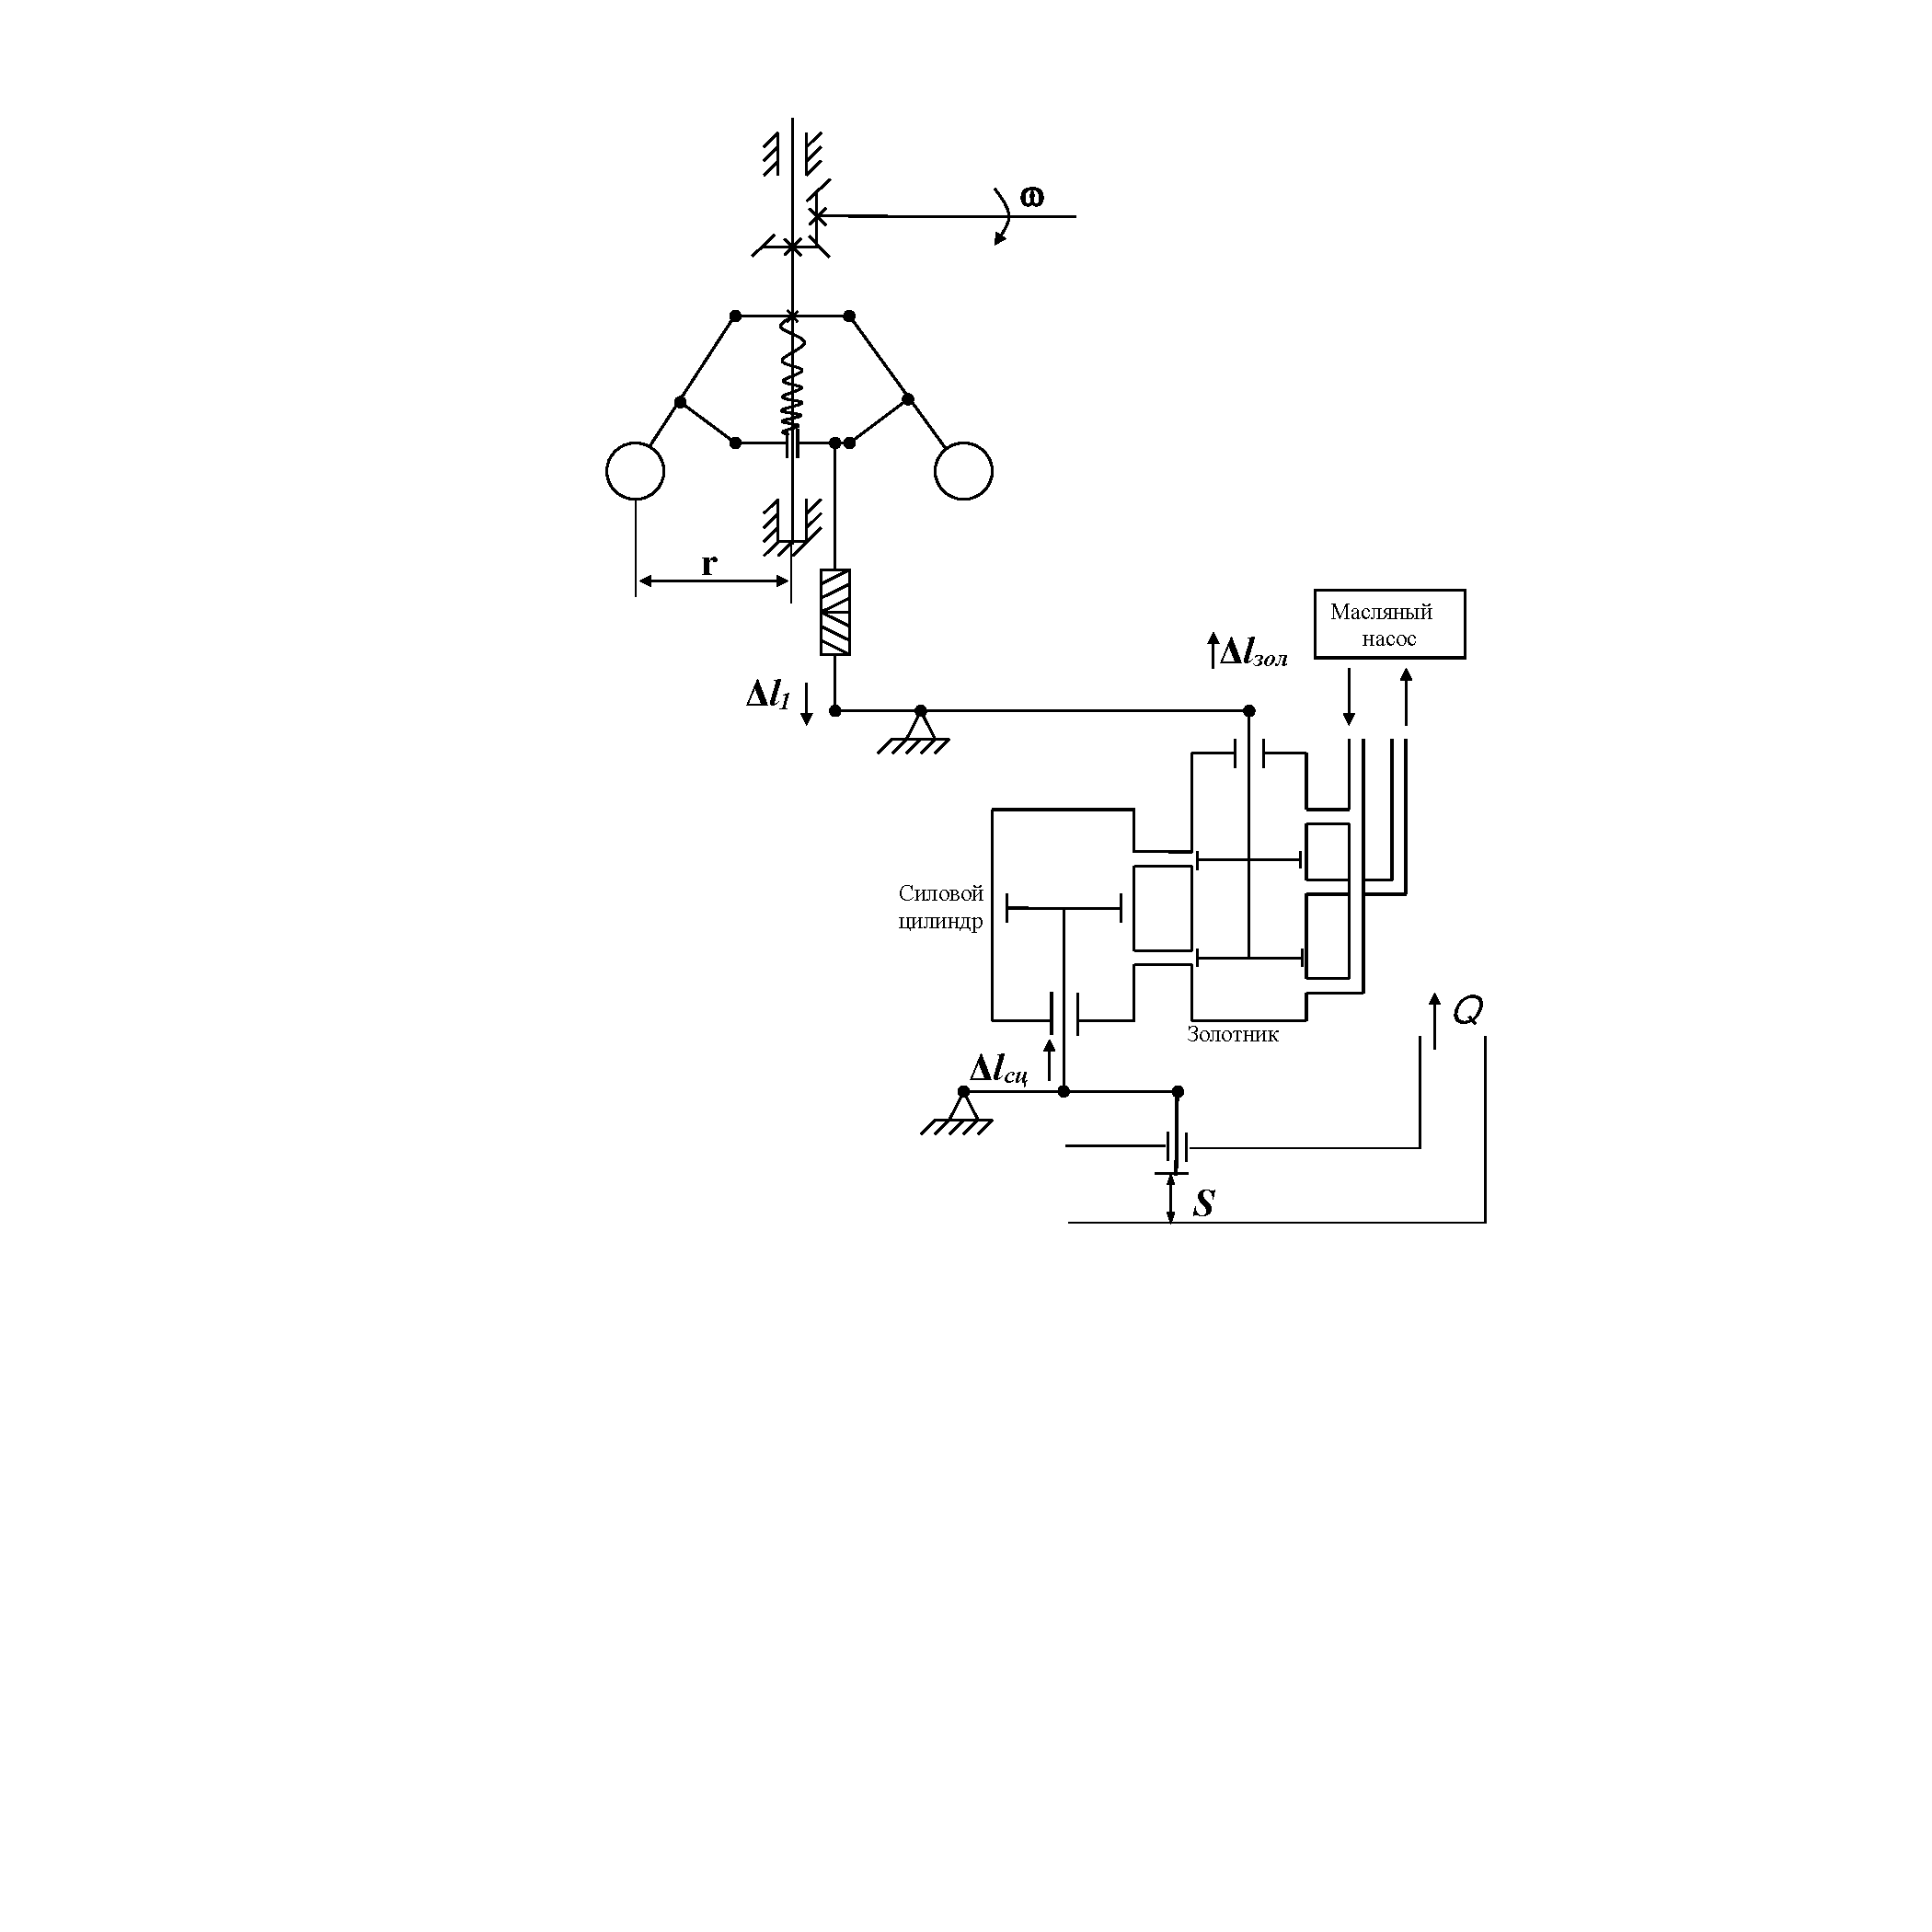
\includegraphics[scale=0.99]{images/TheTurbineController}
	\caption{Регулятор системы стабилизации скорости турбины 
		с использованием гидравлического усилителя}
	\label{fig:theturbinecontroller}
\end{figure}

Для этого в систему введен гидравлический усилитель, включающий в себя золотник, силовой цилиндр и масляный насос. Такая си-стема, в которой энергия регулятора потребляется от отдельного источника, называется \textit{системой непрямого действия}.

При заданной скорости расстояние между грузиками центробежного регулятора равно номинальному значению ($ r=r_{0} $), положение плеча золотника $ l_{зол} $ также равно номинальному значению $ (l_{зол}=l_{зол 0}) $ , при этом поршень золотника полностью перекрывает выходные отверстия, следовательно, положение поршня силового цилиндра неизменно.

С увеличением нагрузочного момента $ M_{Н} $ падают обороты турбины $ \omega $, что приводит к уменьшению расстояния $ $
между грузиками центробежного регулятора. В результате изменяет-ся положение поршенька золотника. Это, в свою очередь, приводит к перемещению поршня силового цилиндра, а следовательно, и к дополнительному приоткрытию заслонки $ S $.Соответственно увеличивается расход пара, возрастает скорость оборотов турбины $ \omega $ и увеличивается расстояние $ r $. Статика (установившееся состояние) в системе возможна только тогда, когда
$ l_{2}=l_{2_{0}} $, то есть когда полностью перекрыты перепускные отверстия золотникового устройства.

Теоретически в этой системе статическая ошибка равна нулю, то есть данная система является \textit{астатической}. В ней отсутствует статическая связь между скоростью и положением заслонки.

Рассмотрим упрощенные уравнения системы. Начнём с уравнения объекта. Очевидно, что изменение скорости турбины может про-исходить лишь в тех случаях, когда нарушается равновесие между движущим моментом турбины $ M_{Т} $и моментом нагрузки $ M_{Н} $:
\begin{equation}\label{eq:ObjectTurbine}
J\cfrac{d\Delta \Omega}{dt}=\Delta  M_{Т}-\Delta  M_{Н}
\end{equation}
где $ J $ --- суммарный момент инерции, приведённый к валу турбины.

С целью упрощения в уравнении (\ref{eq:ObjectTurbine}) использованы приращения скорости и моментов. Более подробно такой подход будет рас-смотрен в разделе, посвященном линеаризации систем.

Будем полагать, что приращение момента турбины пропорционально приращению количества подаваемого пара
\begin{equation*}
	\Delta  M_{Т}=K_{Т}\Delta  Q
\end{equation*}



Запишем уравнение центробежного регулятора. Полагая, что сами отклонения скорости и вызванные ими приращения внутренних переменных регулятора малы, мы можем выразить все зависимости в линейном виде. Тогда приращения скорости раскрытия грузиков и изменение положения поршенька золотника будут связаны линейными зависимостями: 
\begin{align}\label{eq:centrifugalController}
	&\Delta  r=K_{\omega}\cdot\Delta \omega~;\\\nonumber
	&\Delta  l_{зол}=-K_{r}\cdot\Delta  r.
\end{align}

Составляя уравнение гидравлического усилителя, учтём, что скорость перемещения поршня силового цилиндра пропорциональна величине открытия перепускных отверстий золотника, то есть приращению $ l_{зол} $:

\begin{equation}\label{eq:hydraulic}
	\frac{d\Delta  l_{сц}}{dt}=K_{зол}\cdot\Delta  l_{зол}.
\end{equation}

Приращение координаты штока силового цилиндра повлечет за собой изменение положения заслонки и, следовательно, изменение количества подаваемого в турбину пара:	

\begin{equation}\label{eq:DeltaQ}
	\Delta  Q=K_{сц}\cdot\Delta  l_{сц}.
\end{equation}

Продифференцировав уравнение (\ref{eq:DeltaQ}) и учитывая уравнения для центробежного регулятора (\ref{eq:centrifugalController}) и гидравлического усилителя (\ref{eq:hydraulic}), получим уравнение для регулятора:

\begin{equation}
	\frac{d\Delta  Q}{dt}=-K_{р}\cdot\Delta \omega,
\end{equation}
где $ К_{р}=K_{сц}\cdot K_{Зол}\cdot K_{r}\cdot K_{\omega} $ --- коэффициент регулятора.

Запишем совместно уравнения объекта и регулятора

\begin{equation*}
	\begin{cases}
		\cfrac{d\Delta \Omega}{dt}=k_{q}\cdot\Delta -K_{Н}\cdot\Delta  M_{н};\\
		\cfrac{d\Delta  Q}{dt}=-K_{р}\cdot\Delta \omega,
	\end{cases}
\end{equation*}
продифференцируем первое уравнение и подставим в него второе: 
\begin{equation*}
\cfrac{d^{2}\Delta \omega}{dt^{2}}=K_{q}(-K_{р}\cdot\Delta \Omega)-K_{Н}\cfrac{d\Delta  M_{Н}}{dt}~.
\end{equation*}
При условии постоянства нагрузки получаем уравнение свободного движения всей системы
\begin{equation}\label{eq:freedom}
	\cfrac{d^{2}\Delta \omega}{dt^{2}}+K\cdot\Delta \omega=0,
\end{equation}
где
\begin{equation*}
	K=K_{р}\cdot K_{q}.
\end{equation*}
Соответствующее характеристическое уравнение имеет вид 
\begin{equation*}
	\lambda ^{2}+K=0,
\end{equation*}
его корни - $ \lambda _{1,2}=\pm j\sqrt{K}, $

Таким образом, решение уравнения (\ref{eq:freedom}) имеет вид
\begin{equation}\label{eq:undampedOscillations}
	\Delta \omega(t)=C_{1}e^{\lambda _{1}t}+C_{2}e^{\lambda _{2}t}=A\sin(\sqrt{K}\cdot t+\varphi),
\end{equation}
где $ A \text{ и } \varphi $ определяются начальными условиями.

В результате решения получили, что в данной системе в принципе не существует установившегося (статического) состояния. Следовательно, система неработоспособна.

С целью успокоения незатухающих колебаний (\ref{eq:undampedOscillations}) введём в си-стему демпфер (рис.~\ref{fig:thesystemcontrollers}) и рассмотрим, что в ней происходит при изменении нагрузки. С увеличением нагрузочного момента $ M_{Н} $ уменьшается скорость вращения турбины $ \omega $, что приводит 
к уменьшению расстояния $ r $ между грузиками центробежного регулятора. Это влечет за собой изменение положения поршенька золотника $ \Delta  l_{зол} $, а следовательно, и изменение положения поршня силового цилиндра. При этом одновременно происходит два процесса.

Во-первых, вместе со штоком силового цилиндра опускаются поршень и цилиндр демпфера, уменьшая первоначальное изменение $ \Delta  l_{зол} $. Скорость перемещения поршня демпфера относительно его цилиндра невелика и регулируется с помощью специального дросселя Др.

Во-вторых, приоткрывается заслонка, увеличивая количество подаваемого в турбину пара, и начинает расти скорость $ \omega $.

За счёт первого движения поршни золотника могут перекрыть перепускные отверстия ещё до восстановления номинального значения $ \omega $. В то же время пружины стремятся вернуть демпфер в исход-ное положение, и, в конечном итоге, $ \Delta  l_{2} $ стремится к нулю. Теперь уже перепускные отверстия золотника будут перекрыты только при номинальной скорости. Следовательно, система с демпфером, как и предыдущая, является астатической.
Рассмотрим, как повлияло введение демпфера на незатухающие колебания, выявленные в предыдущем варианте системы. Считая отклонения от номинального режима малыми, запишем уравнения эле-ментов регулятора. Как и раньше,
%Изменил, так вроде лучше выглядит
\begin{align}\label{eq:TwoEquation}
	&\Delta  r=K_{\omega}\Delta \omega,\\\nonumber
	&\Delta  l_{1}=-K\cdot\Delta  r;\\
	&	\cfrac{d}{dt}l_{сц}=K_{зол}\Delta  l_{зол}.\label{eq:3eq}
\end{align}
%\begin{equation}
%
%\end{equation}

\begin{figure}[p]
	\centering
	\includegraphics[scale=0.99]{images/TheSystemControllers}
	\caption{Регулятор системы стабилизации скорости турбины 
		с использованием успокоительного демпфера}
	\label{fig:thesystemcontrollers}
\end{figure}

В отличие от предыдущей системы, в данном случае положение штока золотника зависит не только от центробежного регулятора, но и от демпфера:
\begin{equation}\label{eq:PistonRod}
	\Delta  l_{зол}=K_{1}\cdot\Delta  l_{1}-K_{2}\cdot\Delta  l_{2}.
\end{equation}
Упрощенные уравнения демпфера основываются на равенстве сил пружин:
%TT Что то тут не так 
\begin{equation*}
	\Delta  F_{пр}=K_{пр}\cdot\Delta  l_{2}.
\end{equation*}
и сил, связанных с перемещением поршня демпфера относительно корпуса:

\begin{equation*}
	F_{д}=k_{д}\cfrac{d(l_{сц}-l_{2})}{dt},
\end{equation*}
или
\begin{equation*}
	\frac{K_{д}}{K_{пр}}\cdot p\Delta  l_{2}=\cfrac{K_{д}}{K_{пр}}\cdot p\Delta  l_{сц}.
\end{equation*}
Таким образом, изображения перемещений штока силового цилиндра и корпуса демпфера связаны соотношением
\begin{equation}
	\Delta  l_{2}=\cfrac{T_{д}p}{Т_{д}p+1}\cdot\Delta  l_{сц},
\end{equation}
где постоянная времени демпфера
\begin{equation*}
	T_{д}=K_{д}/К_{пр}.
\end{equation*}
Из (\ref{eq:3eq}) и (\ref{eq:PistonRod}) следует
\begin{equation*}
	p\cdot \Delta  l_{сц}=K_{зол}\cdot\left(K_{1}\Delta  l_{1}-K_{2}\cfrac{T_{д}p}{T_{д}p+1}\Delta  l_{сц}\right),
\end{equation*}
откуда
\begin{equation}\label{eq:RavenstoChtoto}
	\left( 1+K_{зол}K_{2}\cfrac{T_{д}}{T_{д}p+1}\right)\cdot p\cdot\Delta  l_{сц}=K_{зол}K_{1}\Delta  l_{1}.
\end{equation}
Используя равенства (\ref{eq:TwoEquation}), (\ref{eq:RavenstoChtoto}) и (\ref{eq:DeltaQ}), получим связь между входом регулятора $ \Delta \Omega $и его выходом $ \Delta  Q $:
\begin{equation}\label{eq:TheRelationship}
	\cfrac{T_{1}p+1}{T_{д}p+1}K_{q\,рег.}p\Delta  Q=K_{зол}K_{1}(-K_{r}K_{\omega})\Delta \Omega,
\end{equation}
где
\begin{equation*}
	K_{q\,рег.}=\cfrac{1+K_{зол}K_{2}T_{д}}{K_{сц}};\quad T_{1}=\cfrac{T_{д}}{1+K_{зол}K_{2}T_{д}}.
\end{equation*}
Если $ T_{1}<<T_{д} $, то \eqref{eq:TheRelationship} упрощается:
\begin{equation*}
	\cfrac{K_{q\, рег}\cdot p}{T_{д}p+1}=-K_{\omega\,рег.}\Delta \omega
\end{equation*}
Это равенство можно решить относительно $ \Delta  Q $:
\begin{equation*}
	\Delta  Q=\cfrac{K_{\omega\,рег.}T_{д}}{K_{q\, рег.}};\quad K_{рег.интегр.}=\cfrac{K_{\omega\,рег.}}{K_{q\,рег.}}
\end{equation*}
и окончательно получим уравнение регулятора, в котором выходная величина $ \Delta  Q $ формируется как сумма пропорциональной и интегральной составляющих ошибки стабилизации $ \Delta  \omega $:
\begin{equation}\label{eq:RegulatorEq}
\Delta  Q=-K_{рег.пропорц.}\cdot\Delta \omega-K_{рег.интегр.}\cfrac{\Delta \omega}{p}
\end{equation}

Запишем уравнение объекта (турбины) относительно изображений по Лапласу его входной и выходной переменных:
\begin{equation}
	p\cdot\Omega=K_{q}\Delta  Q-K_{Н}\Delta  M_{Н}.
\end{equation}
Продифференцируем последнее равенство и подставим в него уравнение регулятора \eqref{eq:RegulatorEq}. В результате получим уравнение системы в целом:
\begin{equation}\label{eq:difirencialTurbina}
p^{2}\Delta \omega+K_{q}K_{рег.пропорц.}\cdot\Delta \omega+K_{q}K_{рег.интегр.}\Delta \omega=-K_{Н}\cdot p \cdot\Delta  M.
\end{equation}
Корни соответствующего характеристического уравнения
\begin{equation*}
	p_{1,2}=-0.5K_{q}K_{рег.пропорц}\pm\sqrt{(0.5K_{q}K_{рег.пропорц.})^{2}-K_{q}K_{рег.интегр.}}
\end{equation*}
всегда имеют отрицательные вещественные части. Это означает, что в отличие от предыдущего случая свободная составляющая решения уравнения \eqref{eq:difirencialTurbina} с течением времени стремится к нулю. Таким образом, введение демпфера позволило получить устойчивую, работоспособную систему.

Разработчики первых систем автоматического регулирования столкнулись со случаями катастрофической неустойчивости, 
на первый взгляд, безукоризненных систем. В 1845 году братья Вильям и Вернер Сименсы предложили метод регулирования 
по производной. Существо их предложения можно пояснить на примере следящей системы, функциональная схема которой
приведена на рис.1.8. На рис.1.9 представлен фрагмент переходных процессов по выходной координате $ \varphi_{вых} $,рассогласованию  (ошибке) $\varepsilon  $ и производной рассогласования $ \dot{\varepsilon} $.Хотя в точках А1 и А2, В1 и В2 отклонения выходной  координаты от входной соответственно равны, управляющие воздействия на объект должны быть различными, так как в точках А1 и В2 выходная координата движется к требуемому значению, а в точках В1 и А2 - удаляется от него. Учитывая инерционные свойства объекта, целесообразно в формирователе закона управления реализовать управлявшее воздействие $ U $, пропорциональное сумме $ \alpha_{1}\varepsilon+\alpha_{2}\dot{\varepsilon} $. Добавление сигнала производной уменьшит абсолютную величину управления в точках А1 и В2 и увеличит её в точках B1 и A2.

Распространение автоматических регуляторов вызвало потребность в разработке теоретически обоснованных методов их расчета. В 1866 году выходит в свет статья Д.К.Максвелла "О регуляторах В 1876 году появилась работа, оказавшая большое влияние на науку о регулировании - труд профессора И.А. Вышнеградского "Об общей теории регуляторов В этой работе было выведено условие устойчивости для линейных систем третьего порядка и даны конкретные указания о том, как влияют конструктивные параметры на устойчивость. И.А. Вышнеградский явился основоположником классической теории регулирования. Работы Вышнеградского были продолжены словацким учёным А. Стодолой. По его просьбе швейцарский математик А. Гурвиц в 1895 году ввел алгебраические условия устойчивости для линейных систем любого порядка. Долгое время оставалась неизвестной инженерам аналогичная работа Е.Д.Рауса, выполненная им еще в 1877 году по просьбе Д.К.Максвелла.

Рис. 1.9. К введению производной ошибки в закон регулирования



		Рис. 1.9. К введению производной ошибки



		в закон регулирования



\bigskip


		Большой вклад в теорию автоматического регулирования внес из­вестный русский ученый Н.Е. Жуковский. В 1880 году вышла
		его работа "О прочности движения". Он читал лекции по теории регуляторов в Московском университете, Математическом
		обществе и Московском тех­ническом училище. В 1909 году вышел его учебник по классической теории регулирования -
		"Теория регулирования хода машин".



		Основы общей теории устойчивости динамических систем были за­ложены выдающимся русским учёным А.М. Ляпуновым. В своей
		докторской диссертации в 1892 году им впервые были сформулированы условия ус­тойчивости решений обыкновенных
		дифференциальных уравнений, дано строгое определение понятия устойчивости, разработаны два основных метода исследования
		устойчивости: первый метод Ляпунова исследования устойчивости в малом и второй, прямой метод исследования устойчивости
		в большом.



		\ В те годы, по-видимому, еще никто не подоз­ревал о будущей роли теории А.М. Ляпунова в общей теории управления. Лишь в
		40-50 годах его теоремы заработали в полную силу.



		В 1932 году американский учёный Х.Найквист разработал теорию устойчивости усилителей с обратной связью. В 1936 году
		молодой со­ветский ученый А.В. Михайлов распространил критерии Найквиста на системы автоматического регулирования и
		предложил свой собственный критерий устойчивости, который с тех пор называется его именем.



		В 1937 году вышла большая работа советских учёных А.А. Андро­нова, С.Э. Хайкина и других по теории нелинейных колебаний,
		где впервые были введены понятия периодических режимов, автоколебаний, фазового пространства.



		Сороковые годы нашего столетия отмечены бурным развитием час­тотных методов, и большую роль в их пропаганде и внедрении
		в прак­тику проектирования в нашей стране сыграли профессор В.В. Солодовни­ков и его ученики, в это же время Н. Винер и
		А.Н. Колмогоров создают теорию синтеза статистически оптимальных систем. В 1948 году К.$ \Phi $ . Теодорчиком в СССР и в 1950
		году \ В.Р.Ивенсом в США закладываются осно­вы теории корневых годографов.



		В 50-60 годы развивается новое перспективное направление - теория оптимального управления. У истоков этой теории стояли
		совет­ские ученые А.А. $ \Phi $ ельдбаум, Л.С. Понтрягин, А.М. Летов, Е.А. Барбашин, А.А. Красовский, Н.Н. Красовский,
		американские учёные Р. Беллман, \ \ \ Р. Калман и другие.



		В 60-е годы М.А. Айзерманом и В.М. Поповым разрабатывается теория абсолютной устойчивости нелинейных систем. Большой
		вклад в теорию импульсных и цифровых систем автоматического управления внесли Ю.Ту, Я.З. Цыпкин, Л.Т. Кузин, Э. Джури.
		В.С. Пугачёв обогатил теорию управ­ления разработкой вопросов статистической динамики. Родоначальником теории
		дифференциальных игр является академик Н.Н. Красовский. Продуктивную работу в области распознавания образов и
		управления в условиях неопределённости ведут \ математики Екатеринбурга. Всемирно известны работы российских учёных
		Б.Н. Петрова и С.В. Емельянова в области те­ории и практики адаптивных систем.



\bigskip


\bigskip


		Теория автоматического управления (ТАУ) – это наука, которая, абстрагируясь от конкретного исполнения различных объектов
		и систем АУ, изучает особенности установившихся и динамических режимов этих систем и предлагает методы проектирования
		управления, обеспечивающего выполнение требований, предъявляемых к ходу управляемого технологического процесса.



		По принципу формирования управления системы автоматического управления (САУ) подразделяются на следующие:


%\liststyleWWviiiNumvii
\begin{itemize}
	\item 
			разомкнутые, 
	
	\item 
			замкнутые,
	
	\item 
			комбинированные.
	
\end{itemize}

		По цели управления САУ подразделяют на системы:



\begin{itemize}
	\item 
			стабилизации,
	
	\item 
			программного управления,
	
	\item 
			следящие.
	
\end{itemize}

		ТАУ работает с математическими моделями объектов системы управления, сочетает анализ и синтез.



		По математическому описанию и по свойствам САУ подразделяются на следующие типы:


%\liststyleWWviiiNumli
\begin{itemize}
	\item 
			обыкновенные системы – системы, которые описываются дифференциальными или разностными уравнениями с сосредоточенными
			параметрами;
	
	\item 
			системы с распределенными параметрами;
	
	\item 
			непрерывные системы – системы, все координаты (переменные) которых являются непрерывными функциями времени;
	
	\item 
			дискретные системы – системы, в которых хотя бы одна из координат (переменных) является импульсной (дискретной или
			решётчатой) функцией времени;
	
	\item 
			детерминированные системы – системы с постоянными или изменяющимися известным (детерминированным) образом параметрами;
	
	\item 
			стохастические системы – системы, параметры которых изменяются во времени случайным образом;
	
	\item 
			линейные системы – системы, которые описываются линейными дифференциальными или разностными уравнениями;
	
	\item 
			нелинейные системы– системы, которые описываются нелинейными дифференциальными или разностными уравнениями;
	
	\item 
			традиционные одноуровневые системы – системы с регулированием только основных переменных;
	
	\item 
			системы с адаптивным управлением, в которых кроме основного контура с отрицательной обратной связью имеется контур,
			оценивающий текущие параметры управляемого объекта и соответствующим образом изменяющий управляющее воздействие или
			перестраиваемые параметры регулятора;
	
	\item 
			оптимальные системы.
	
\end{itemize}

\bigskip


		Более подробная и обстоятельная классификация систем автоматического управления приведена в обширной литературе по
		теории управления. В частности, можно порекомендовать учебник А.А. Красовского и Г.С. Поспелова [7]. 
\chapter{Методы анализа непрерывных систем}
\section{Понятие пространства состояний}



		С точки зрения анализа и синтеза систем все переменные, характеризующие объект управления (рис.\ref{fig:0_10}) %(рис.2.1)
		 или имеющие к нему
		отношение, делятся на три группы.



\bigskip
\begin{figure}[h!]
	\centering
	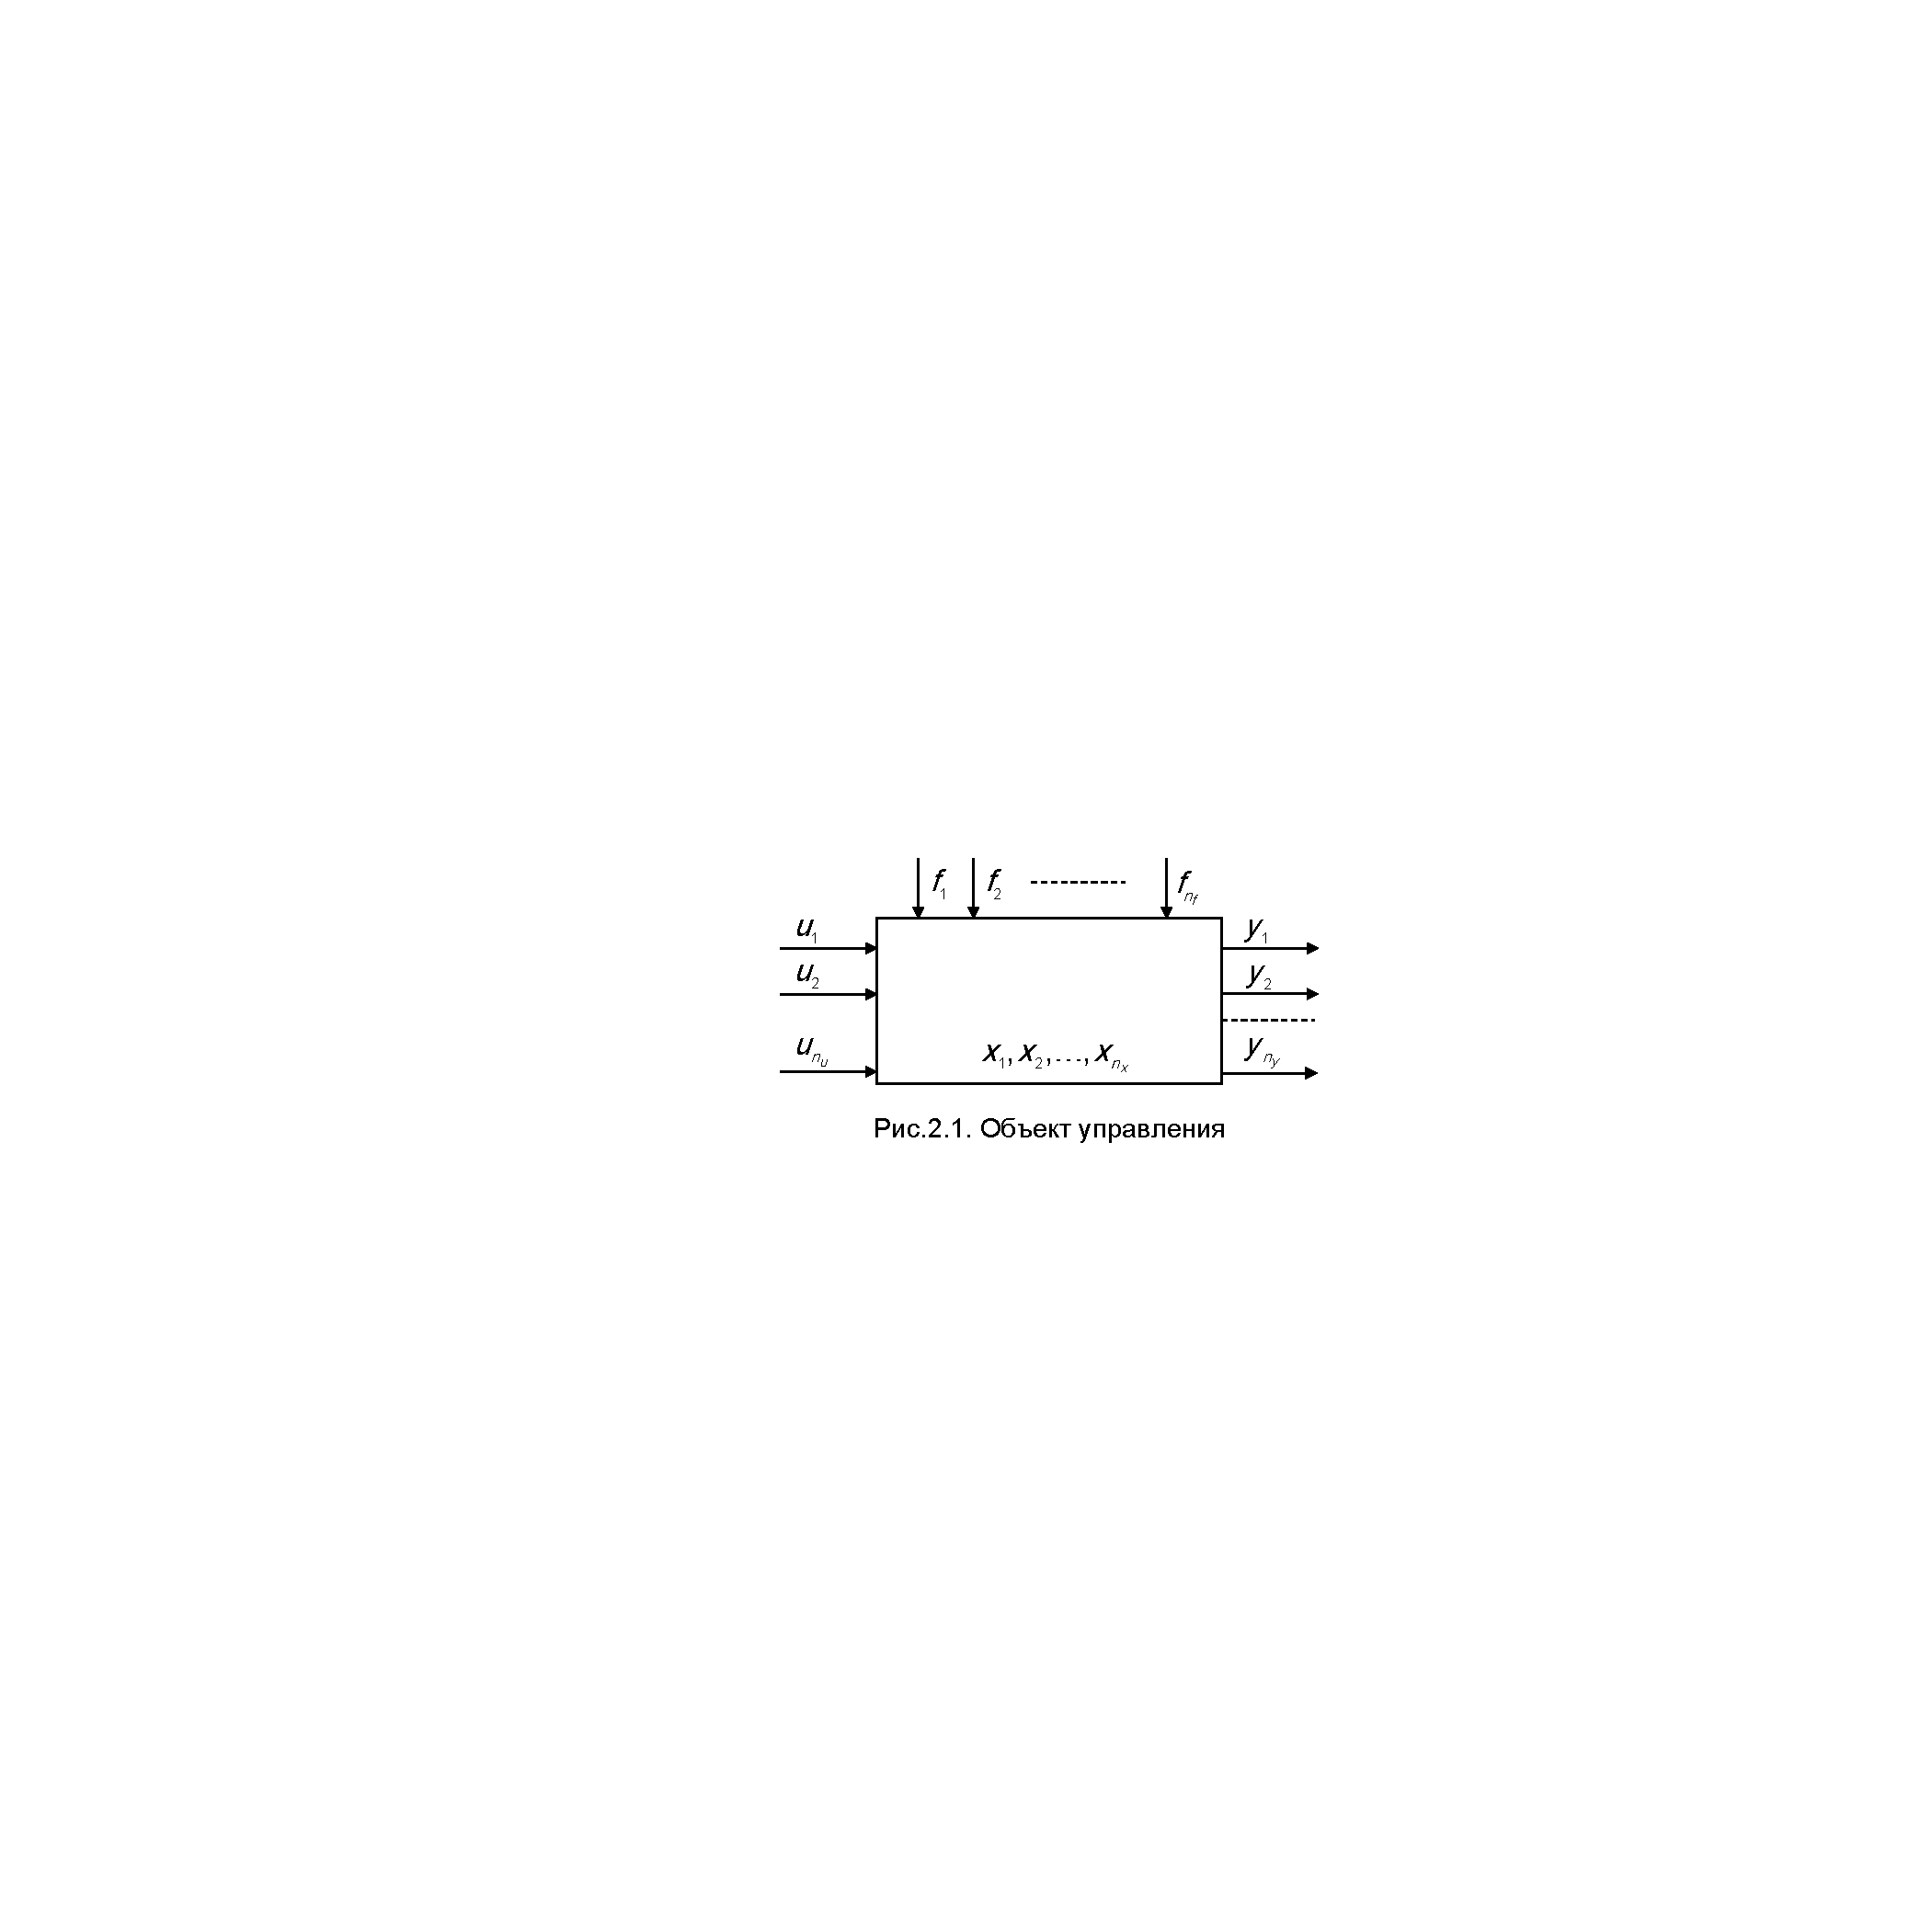
\includegraphics[scale=0.99]{0-10}
	\caption{Объект управления}
	\label{fig:0_10}
\end{figure}


\bigskip


		1.Входные воздействия, представляющие сигналы, генерируемые сис­темами, внешними по отношению к исследуемому объекту, и
		влияющие на его поведение. Внешние сигналы разделяют на сигналы управляющие -  $u_1,u_2,\ldots,u_{n_u}$ и
		возмущающие -  $f_1,f_2,\ldots,f_{n_f}$.



		2.Выходные переменные, или переменные, позволяющие описать некоторые аспекты поведения объекта, представляющие интерес	для иссле­дователя или потребителя результатов функционирования объекта - $y_1,y_2,\ldots,y_{n_y}$.



		3.Переменные состояния, или промежуточные переменные  $x_1,x_2,\ldots,x_{n_x}$, характеризующие динамическое
		поведение исследуемого объекта или системы.



		Для удобства оперирования с многомерными величинами совокупность управляющих переменных представляют в виде вектора
		управления  $\vec u$. Аналогичным образом вводятся понятия вектора возмущения  $\vec f$, вектора выхода  $\vec y$ и
		вектора состояния  $\vec{x}$:



\bigskip

\begin{equation*}
		\vec u=\left(\begin{matrix}u_1\\u_2\\\cdots \\u_{n_u}\end{matrix}\right),  
		\vec f=\left(\begin{matrix}f_1\\f_2\\\cdots\\f_{n_f}\end{matrix}\right),   
		\vec y=\left(\begin{matrix}y_1\\y_2\\\cdots\\y_{n_y}\end{matrix}\right),  
		\vec x=\left(\begin{matrix}x_1\\x_2\\\cdots\\x_{n_x}\end{matrix}\right).
\end{equation*}



\bigskip


		\ \ Множество всех значений, которые может принять вектор  $\vec u$ в момент времени  $t$, образует пространство
		управления. Аналогично вводятся понятия пространства возмущений, пространства выходов и пространства состояний.



		В любой момент времени  $t$ состояние системы является функцией начального состояния  $\vec x(t_0)$ и векторов  $\vec
		u(t_0,t)$ и  $\vec f(t_0,t)$. Если известно, как изменялись эти векторы на интервале  $[t_0,\;t]$, то однозначно может
		быть определено состояние системы  $\vec x(t)$:



\begin{equation}\label{eq:equation_of_state}
		 \vec x(t)=F\{\vec x(t_0),\vec u(t_0,t),\vec f(t_0,t)\}.% (2.1.1)
\end{equation}



		Вектор выхода в момент времени  $t$ является функцией тех же переменных:



\begin{equation}\label{eq:output equation}
		\vec y(t)=\Psi\{\vec x(t_0),\vec u(t_0,t),\vec f(t_0,t)\} %(2.1.2)
\end{equation}



		Состояние системы отделяет будущее от прошлого, так что состояние содержит всю информацию, необходимую для определения
		реакции объекта на произвольный входной сигнал. Понятие состояния является основным исходным понятием и, следовательно,
		не может быть определено более полно, чем, например, слово "множество" в математике. Наибольшее, что можно сделать, это
		сформулировать свойства, какими должна обладать система, поведение которой отвечает понятию состояния.



		Основным свойством состояния является то, что будущие значения его не зависят от характера достижения системой её
		текущего состо­яния. Состояние системы в данный момент времени, а также текущее и будущие значения её входов
		единственным образом определяют настоя­щее и будущие значения её состояния и выходов.



		Уравнение \eqref{eq:equation_of_state} называют уравнением состояния системы, а уравне­ние \eqref{eq:output equation} - уравнением выхода. Если объект
		описывается дифференциаль­ным уравнением, то уравнения \eqref{eq:equation_of_state} и \eqref{eq:output equation} превращаются в



\begin{equation}\label{eq:differential equation of state}
		  \vec{\dot x}(t)=F\{\vec x(t),\vec u(t),\vec f(t),t\}, \  \vec x(t_0)=\vec x_0; (2.1.3)
\end{equation}

\begin{equation}
	y(t)=\Psi\{\vec x(t),\vec u(t),t,\vec v(t)\} (2.1.4)
\end{equation}
		 
		где дополнительно введён вектор ошибок измерений  $\vec v(t)$.



		Как правило, выбор состояния естественным образом следует из физического устройства системы, а уравнение \eqref{eq:differential equation of state}(2.1.3),
		называемое диффе­ренциальным уравнением состояния, обычно следует из элементарных физических законов, которыми
		определяется её поведение.


\section{Линеаризация исходных уравнений}
		Почти все реальные объекты и системы автоматического управления являются нелинейными. Однако среди нелинейных функций 
		$F$ и  $\Psi$ часто встречаются такие, которые при определённых допущениях в рабочей области функционирования системы
		могут быть заменены линейными. В качестве примера такого случая представлена элементарная функция на рис.\ref{fig:2.2}. %2.2
		 В данном
		случае возможна линеаризация, так как если точка  $A$ перемещается на небольшие расстояния по кривой  $V_2=f(V_1)$, то
		этот участок кривой можно заменить \ отрезком прямой. В то же время нелинейная функция на рис.\ref{fig:2.3} %2.3 
		не допускает подобную
		замену, если в процессе работы системы происходит изменение уровня выходного сигнала  $V_2$. Системы с такого типа
		функциями называют \textit{существенно нелинейными}. Их исследованию будет посвящен специальный раздел пособия. Ниже
		будет рассмотрен класс систем, допускающих линеаризацию.




\begin{figure}[h]
	\begin{center}
		\begin{minipage}[h]{0.4\linewidth}
			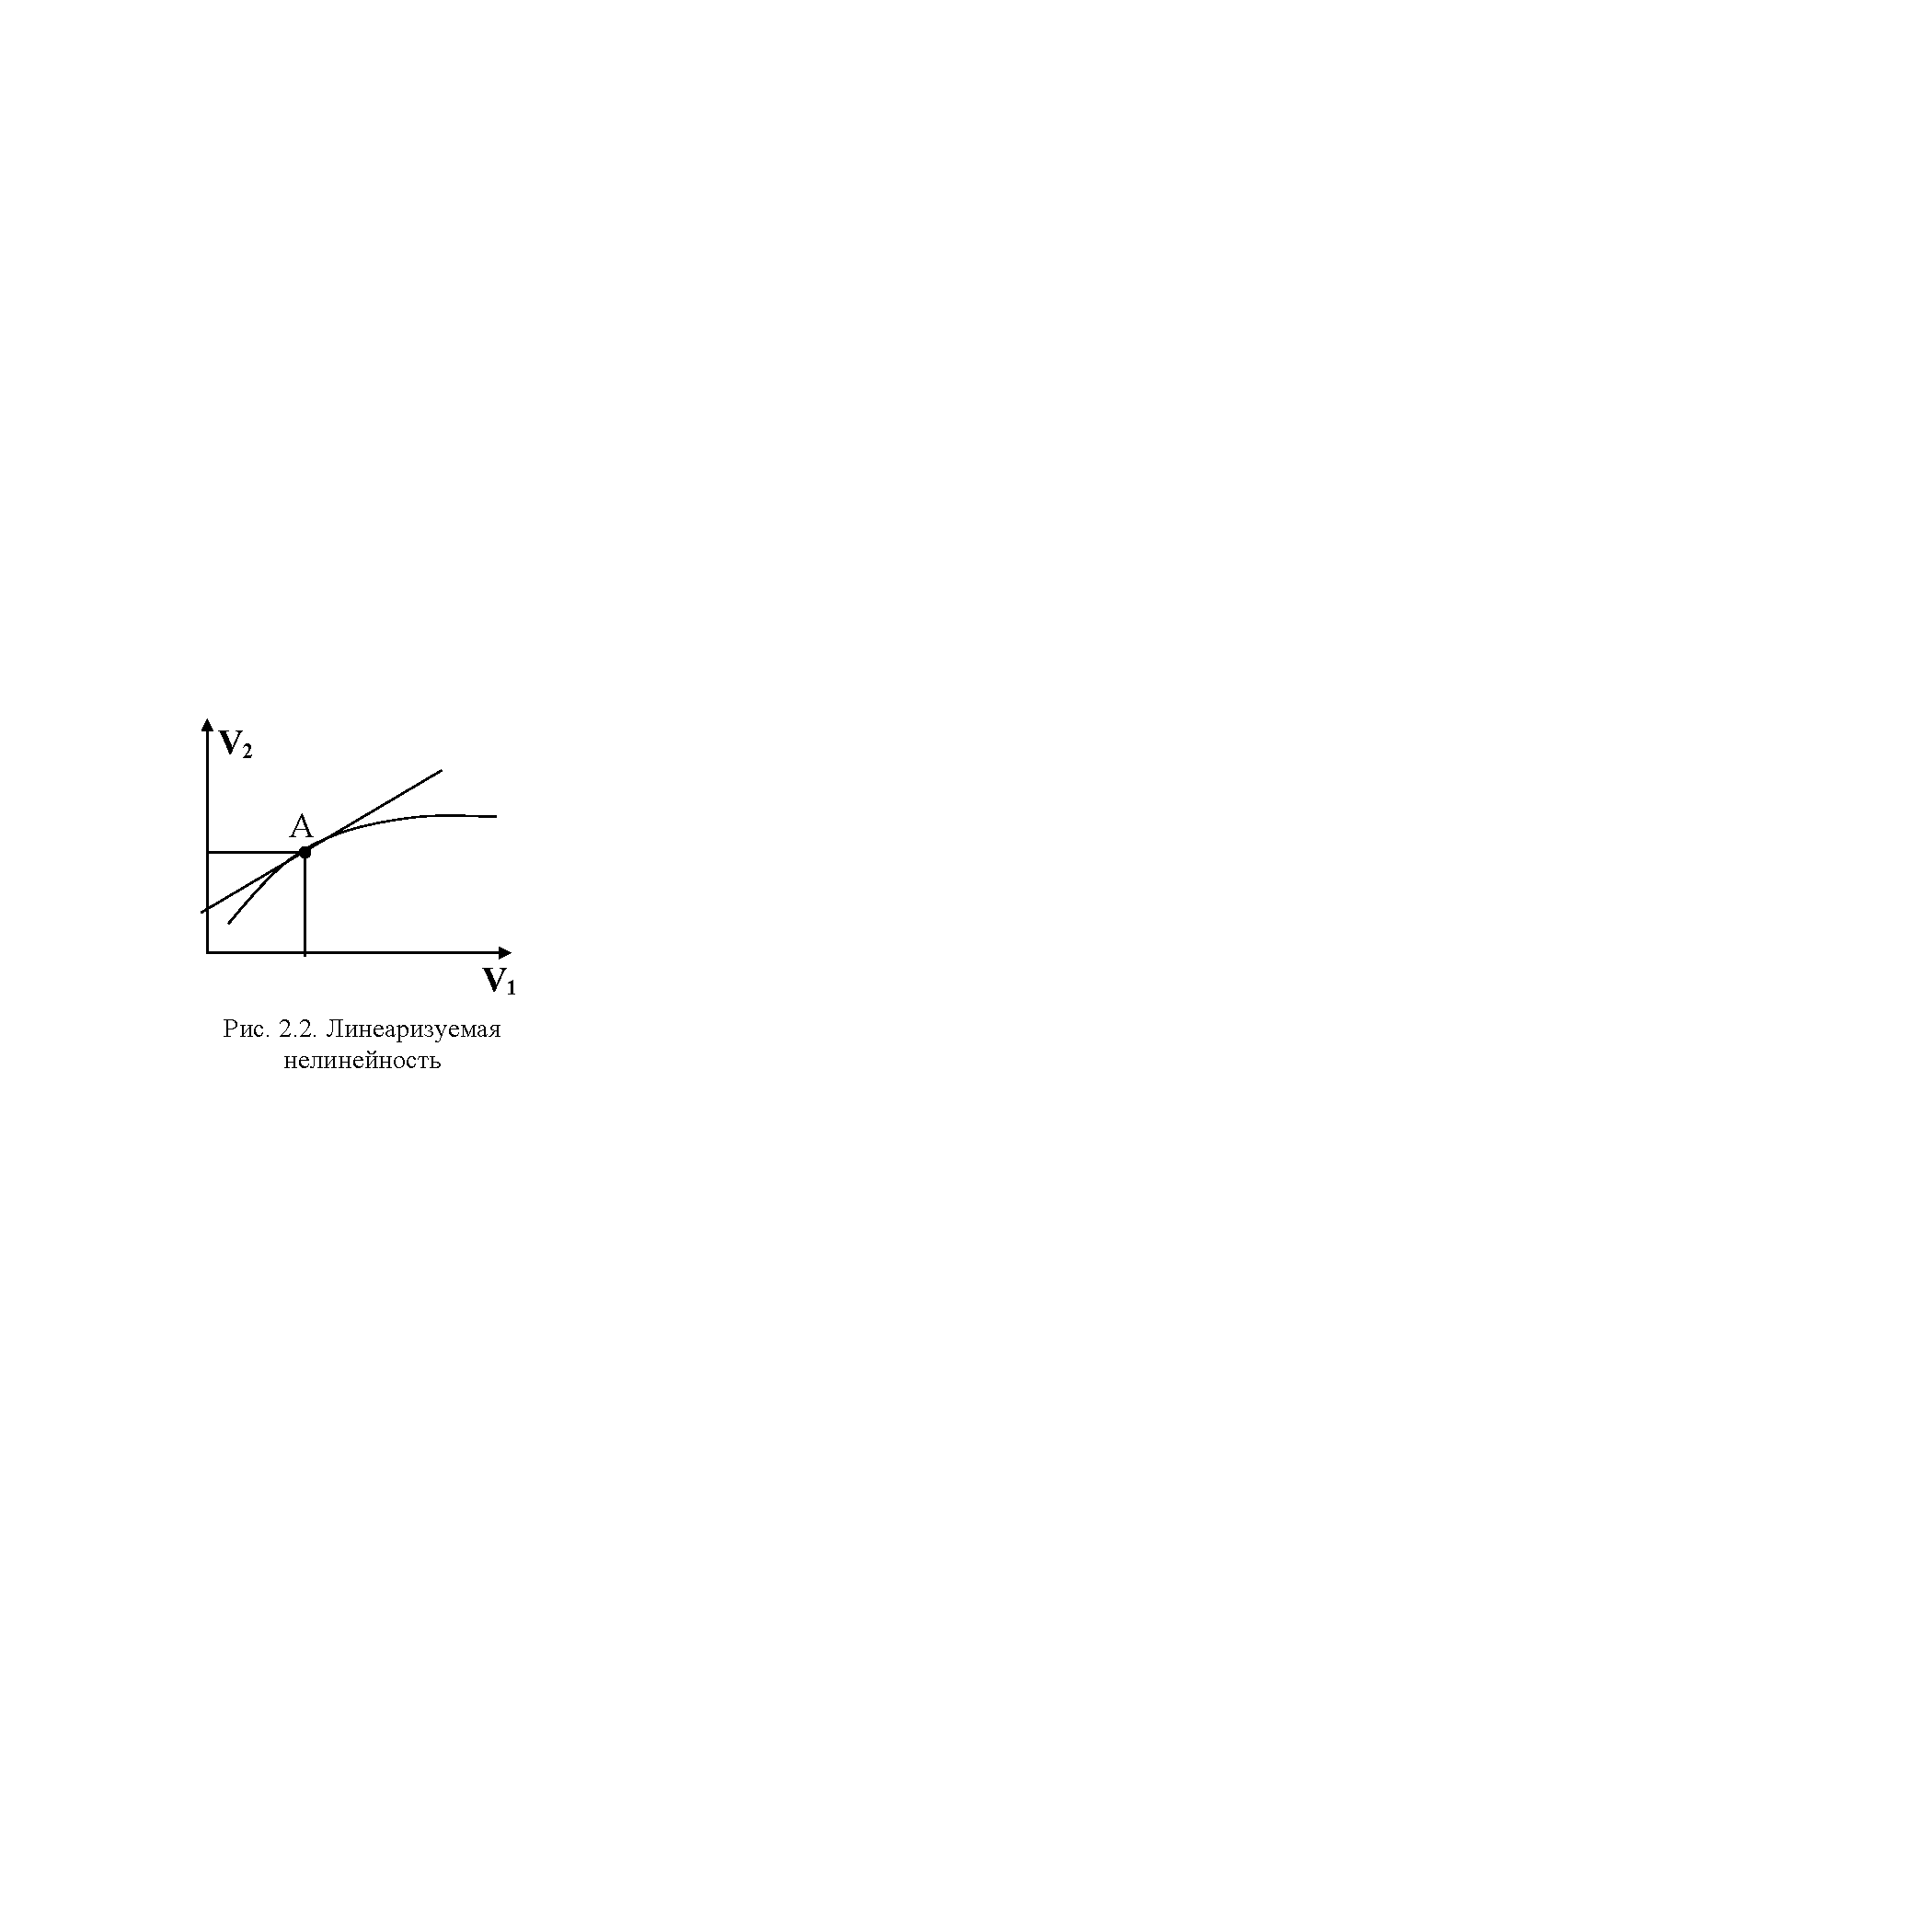
\includegraphics[width=1\linewidth]{img-011}
			\caption{Линеаризуемая нелинейность } %% подпись к рисунку
			\label{fig:2.2} %% метка рисунка для ссылки на него
		\end{minipage}
		\hfill 
		\begin{minipage}[h]{0.4\linewidth}
			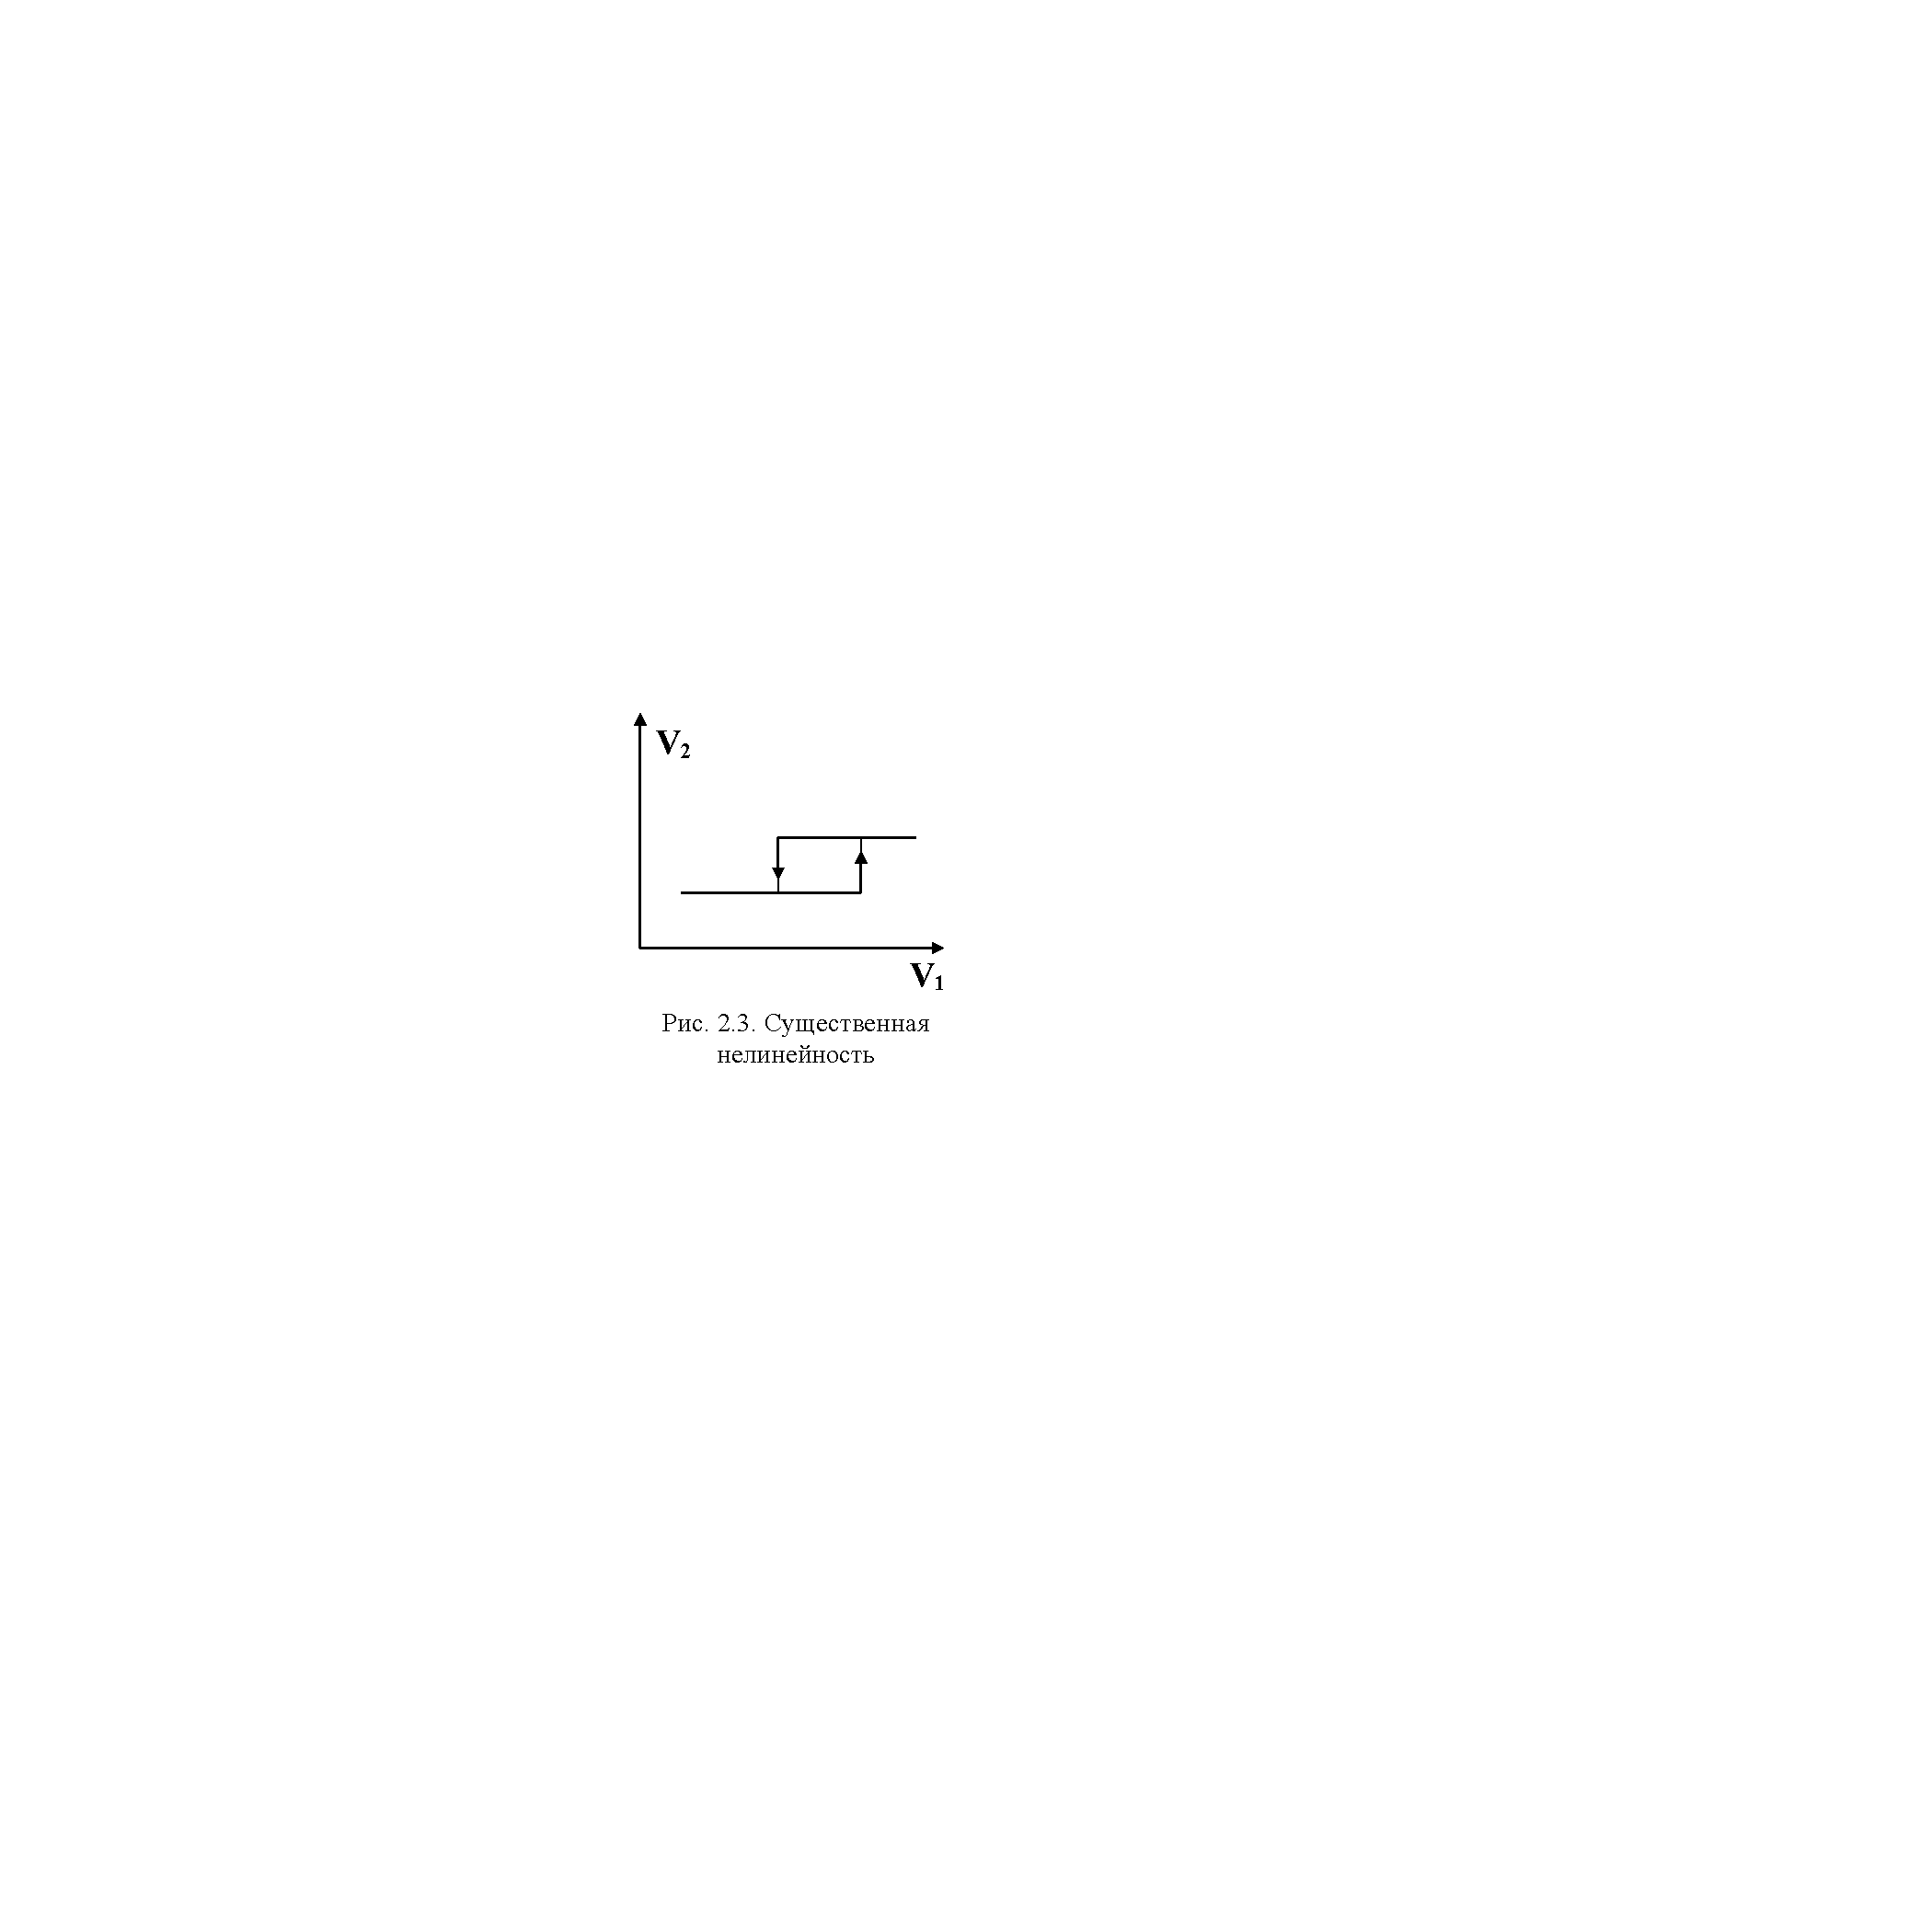
\includegraphics[width=1\linewidth]{img-011b}
			\caption{Существенная  нелинейность}
			\label{fig:2.3}
		\end{minipage}
	\end{center}
\end{figure}


\bigskip


		Пусть режим функционирования объекта определяется некоторой траекторией по вектору управления  $\vec u_0(t)$, а
		действительная реализация  $\vec u(t)$ близка к ней:
	\begin{equation}\label{key}
		 \vec u(t)=\vec u_0(t)+\Delta \vec u(t). %(2.2.1)
	\end{equation}

		При этом \ решение уравнения \eqref{eq:differential equation of state} %(2.1.3) 
		можно записать в виде
\begin{equation}\label{key}
		\vec x(t)=\vec x_0(t)+\Delta \vec x(t), %(2.2.2)
\end{equation}



		где  $\vec x_0(t)$ – решение уравнения  \eqref{eq:differential equation of state} %(2.1.3) 
		при  $\vec u=u_0(t)$.



		Назовём функционирование объекта (системы) при  $\vec u=u_0(t)$ \textit{базовым режимом}. Переменные \  $\Delta \vec
		x(t),\Delta \vec u(t),\Delta \vec f(t)$ – это отклонения от соответствующих переменных в базовом режиме.



		Подставим теперь выражения для  $\vec x(t)$ \ и  $\vec u(t)$ в исходное дифференциальное уравнение состояний


\begin{equation*}
\vec{\dot x}_0(t)+\Delta \vec{\dot x}(t)=F\{\vec x_0(t)+\Delta \vec x(t),\vec u_0(t)+\Delta \vec u(t),\vec f_0(t)+\Delta \vec f(t),t\}
\end{equation*}
		и разложим функцию  $F$ в ряд Тейлора:
\begin{equation}\label{eq:Function F to Tailor}
		\begin{matrix}\vec{\dot x}_0(t)+\Delta \vec{\dot x}(t)=F\{\vec x_0,\vec u_0,\vec f_0,t\}+J_x\{\vec
		x_0,\vec u_0,\vec f_0,t\}\Delta \vec x+\hfill\null \\+J_U\{\vec x_0,\vec u_0,\vec f_0,t\}\Delta \vec u+J_f\{\vec x_0,\vec u_0,\vec
		f_0,t\}\Delta \vec f+R\;.\hfill\null \end{matrix}  % (2.2.3)
\end{equation}



		Здесь  $R$ – остаточный член, содержащий высшие степени приращений, и им можно пренебречь;  $J_x,J_u,\;J_f$ – матрицы
		Якоби функции  $F$ для  $\vec x$,  $\vec u$ и  $\vec f$.

		Элемент матрицы Якоби определяется как со­от­вет­ствующая частная производная 
		$ (J_{x})_{ik}=\frac{dF_{i}}{dx_{k}} $.
		Например, для системы второго порядка соответствующее слагаемое в правой части \eqref{eq:Function F to Tailor} %(2.2.3) 
		имеет вид
\bigskip

\begin{equation*}\label{key}
	J_x\cdot \Delta \vec x=\left[\begin{matrix}\cfrac{\partial F_1}{\partial x_1}&\cfrac{\partial F_1}{\partial
			x_2}\\\cfrac{\partial F_2}{\partial x_1}&\cfrac{\partial F_2}{\partial x_2}\end{matrix}\right]\cdot
		\left[\begin{matrix}\mathit{\Delta x}_1\\\mathit{\Delta x}_2\end{matrix}\right]=\left[\begin{matrix}\cfrac{\partial F_1}{\partial
			x_1}\mathit{\Delta x}_1+\cfrac{\partial F_1}{\partial x_2}\mathit{\Delta x}_2\\\cfrac{\partial F_2}{\partial
			x_1}\mathit{\Delta x}_1+\cfrac{\partial F_2}{\partial x_2}\mathit{\Delta x}_2\end{matrix}\right].
\end{equation*}



\bigskip
		Пренебрегая в  \eqref{eq:Function F to Tailor} %(2.2.3) 
		остаточным членом  $R$ и учитывая уравнение для базового режима, получим
		% тут есть точка или нет? Да есть
\begin{equation}\label{key}
		\Delta \vec{\dot x}(t)=J_x\{\vec x_0,\vec u_0,\vec f_0,t\}\Delta \vec x+J_U\{\vec x_0,\vec u_0,\vec f_0,t\}\Delta \vec u+J_f\{\vec
		x_0,\vec u_0,\vec f_0,t\}\Delta \vec f.\ \ (2.2.4)
\end{equation}
		Введем обозначения:
\begin{equation*}
\begin{matrix}A(t)=J_x\left\{\vec x_0(t),\vec u_0(t),\vec f_0(t),t\right\}\;;\hfill\null \\B(t)=J_u\left\{\vec
x_0(t),\vec u_0(t),\vec f_0(t),t\right\}\;;\hfill\null \\G(t)=J_f\left\{\vec x_0(t),\vec u_0(t),\vec
f_0(t),t\right\}\;.\hfill\null \end{matrix}\hfill 
\end{equation*}

		В результате получим:



		\textit{линейное дифференциальное векторно-матричное уравнение с переменными параметрами} (коэффициентами)
\begin{equation}\label{eq:Dif Mat Vec Eq}
		\Delta \vec{\dot x}(t)=A(t)\cdot \Delta \vec x(t)+B(t)\cdot \Delta \vec u(t)+G(t)\cdot \Delta \vec f(t). %(2.2.5)
\end{equation}
		Аналогичным образом проведем линеаризацию уравнения выхода:
\begin{equation}\label{eq: lean eq exit}
		  \Delta \vec y(t)=C(t)\cdot \Delta \vec x(t)+D(t)\cdot \Delta \vec u(t)+\Delta \vec v(t). %(2.2.6)
\end{equation}

		Впредь, рассматривая линейные модели системы, будем опускать символ $ \Delta $ при записи приращений соответствующих
		векторов. Таким образом, линеаризованные уравнения объекта (системы) примут вид
\begin{align}\label{eq: lean system 1}
		&\vec{\dot x}(t)=A(t)\vec x(t)+B(t)\vec u(t)+G(t)\vec f(t); (2.2.7)\\
		\label{eq: lean system 2}
		&\vec y(t)=C(t)\vec x(t)+D(t)\vec u(t)+\vec v(t).(2.2.8)
\end{align}



		Ha рис. \ref{fig:2_4} %2.4 
		приведена структурная схема, являющаяся графичес­ким изображением уравнений \eqref{eq: lean system 1} %(2.2.7) 
		и \eqref{eq: lean system 2}%(2.2.8)
		.

\begin{figure}[h]
\centering  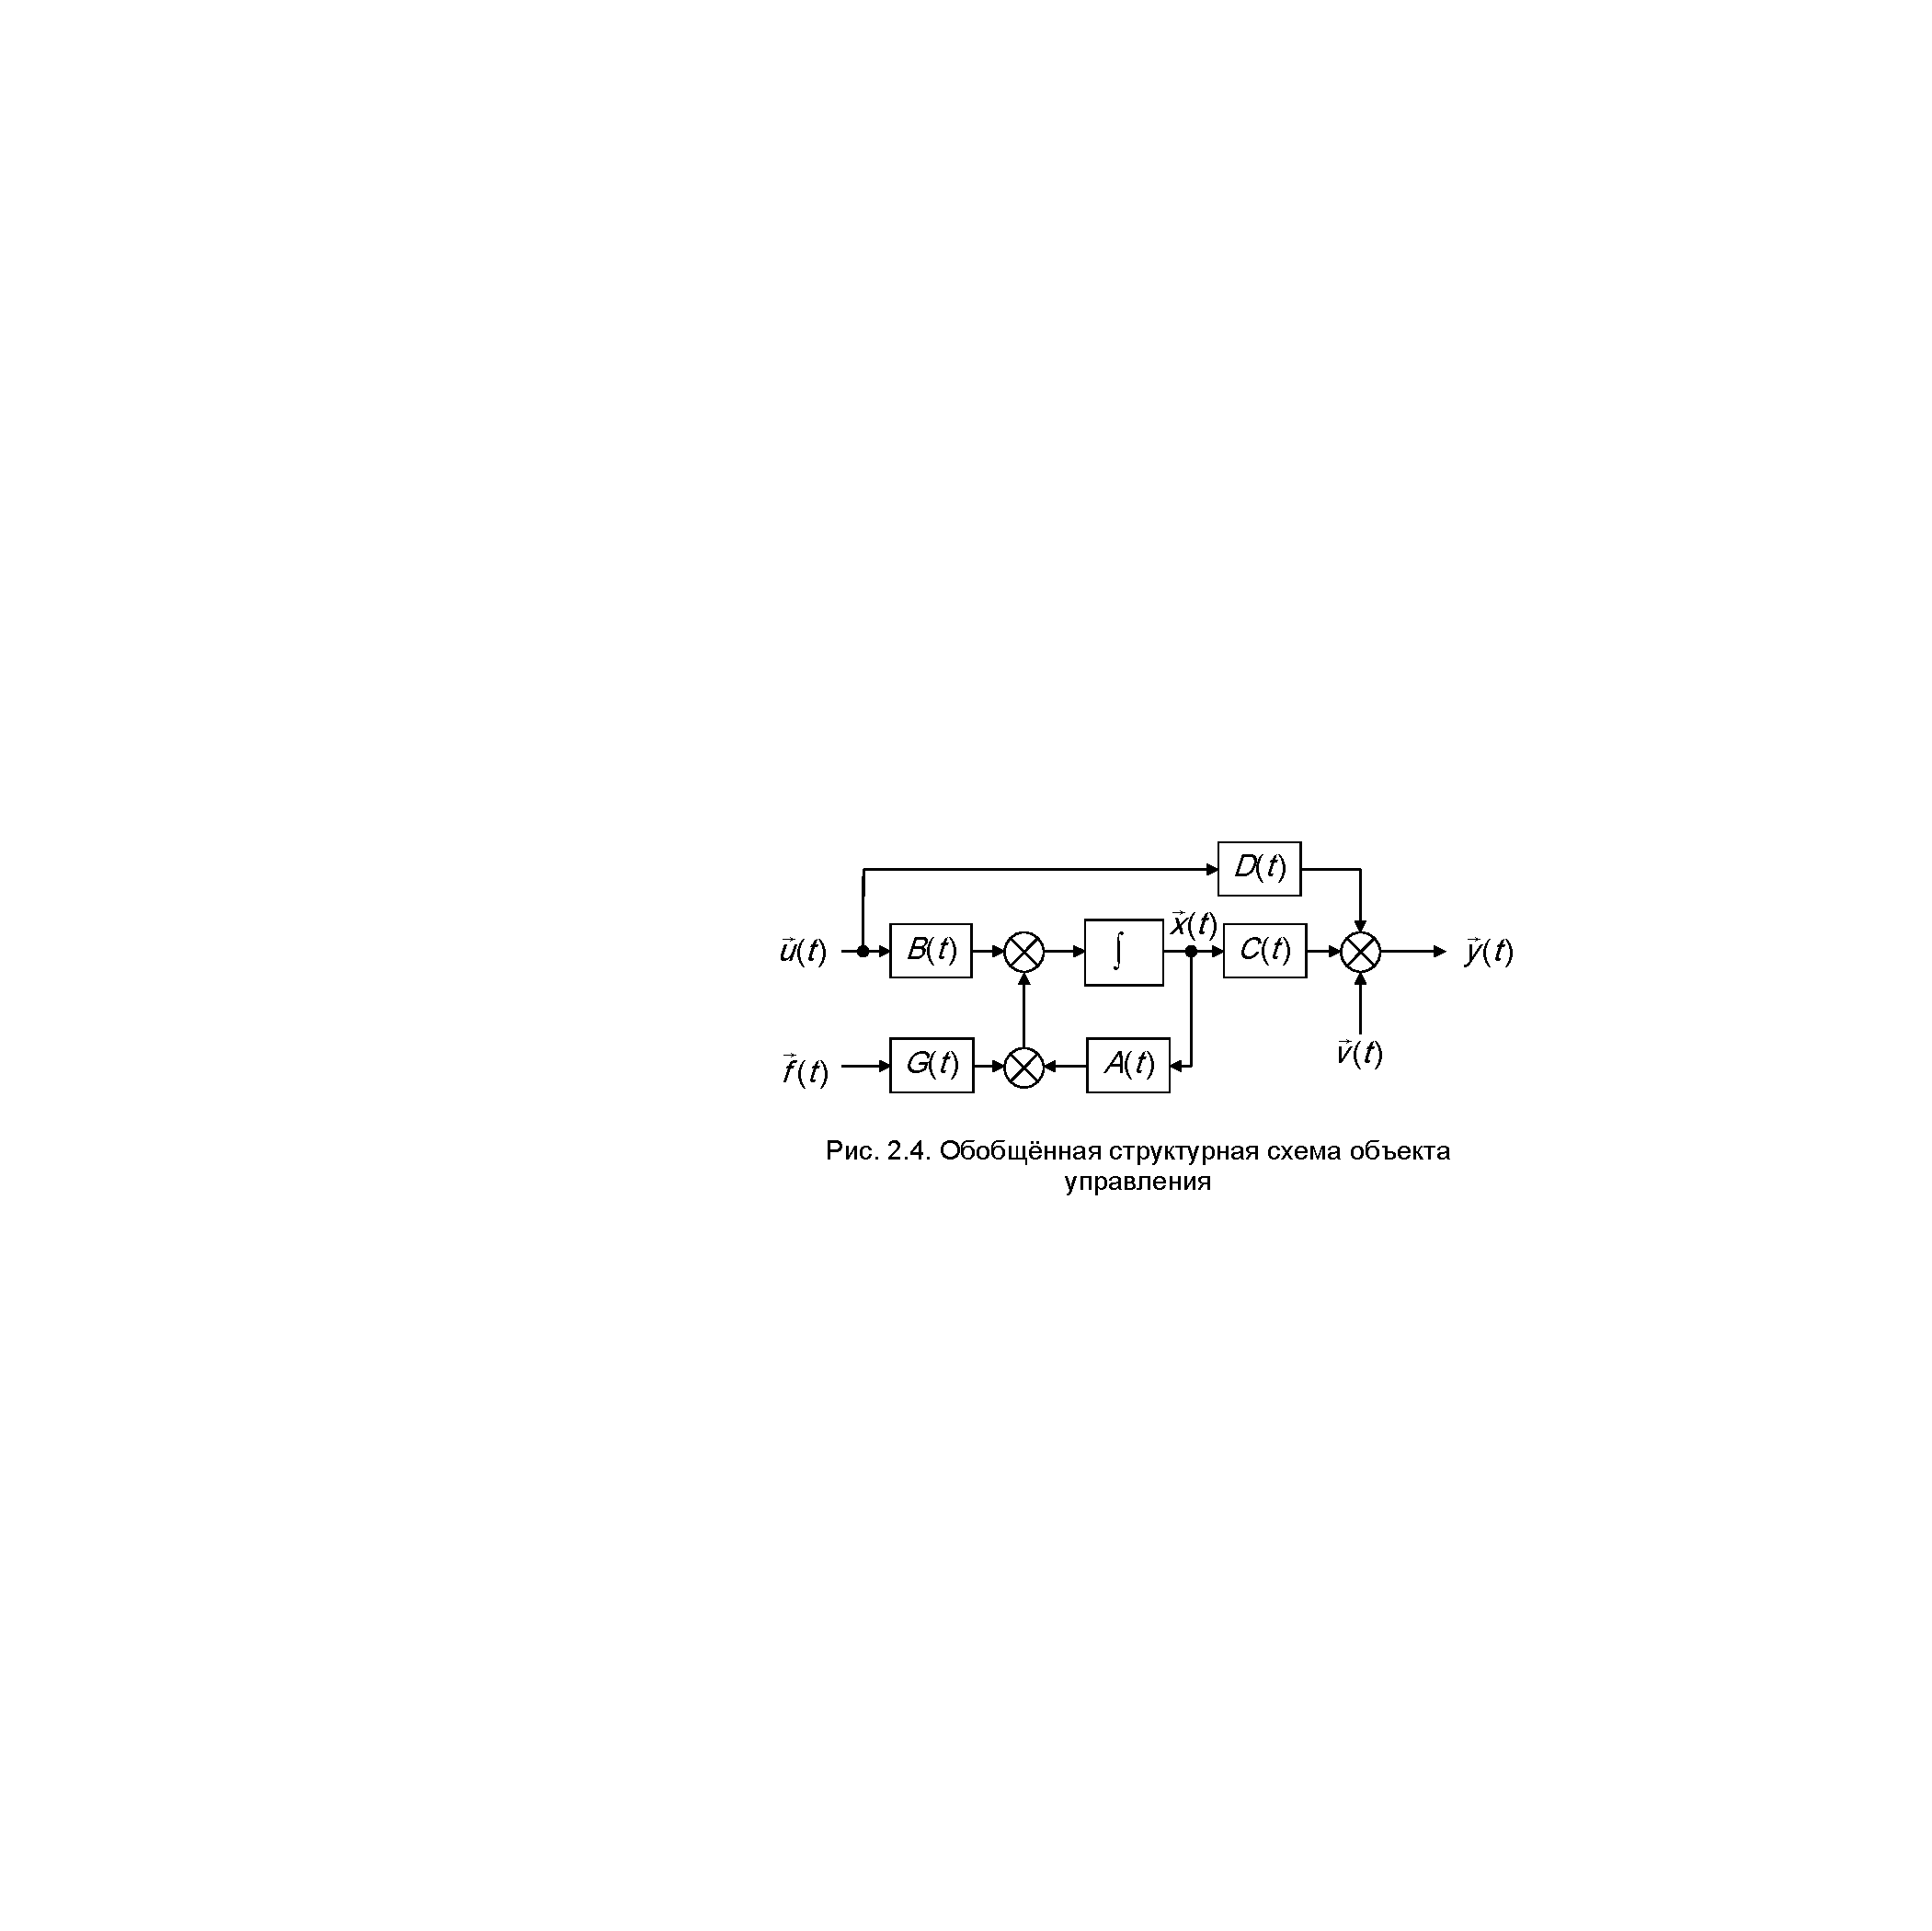
\includegraphics[width=13.679cm,height=6.773cm]{img-012} 
\caption{Обобщённая структурная схема объекта управления}
\label{fig:2_4}
\end{figure}
		В качестве примера рассмотрим смесительный бак, который наполняется с помощью двух потоков, имеющих переменные
		мгновенные расходы  $F_1(t)$ и  $F_2(t)$ (рис. \ref{fig:buc}%2.5
		). Оба входных потока содержат растворимое вещество с неизменными
		концентрациями  $C_1$ и  $C_2$. Выходной поток имеет массовую скорость истечения (мгновенный расход)  $F(t)$.
		Предполагается, что содержимое бака перемешивается так, что концентрациb выходного потока равна концентрации 
		$C_{{\text{out}}}(t)$ в баке.
		
		Запишем уравнения баланса масс в баке.
		
		Для полной массы:



\begin{equation}\label{eq:full mass}
 \frac{\text{dV}(t)}{\text{dt}}=F_{1}(t)+F_{2}(t)-F(t). (2.2.9)
\end{equation}
		Для массы растворённого вещества
\begin{equation}\label{eq:solute}
		 \frac{d}{\text{dt}}\{C_{\text{out}}(t)V(t)\}=C_1F_1(t)+C_2F_2(t)-C_{\text{out}}(t)F(t).(2.2.10)
\end{equation}

\begin{figure}[h]
	\centering
	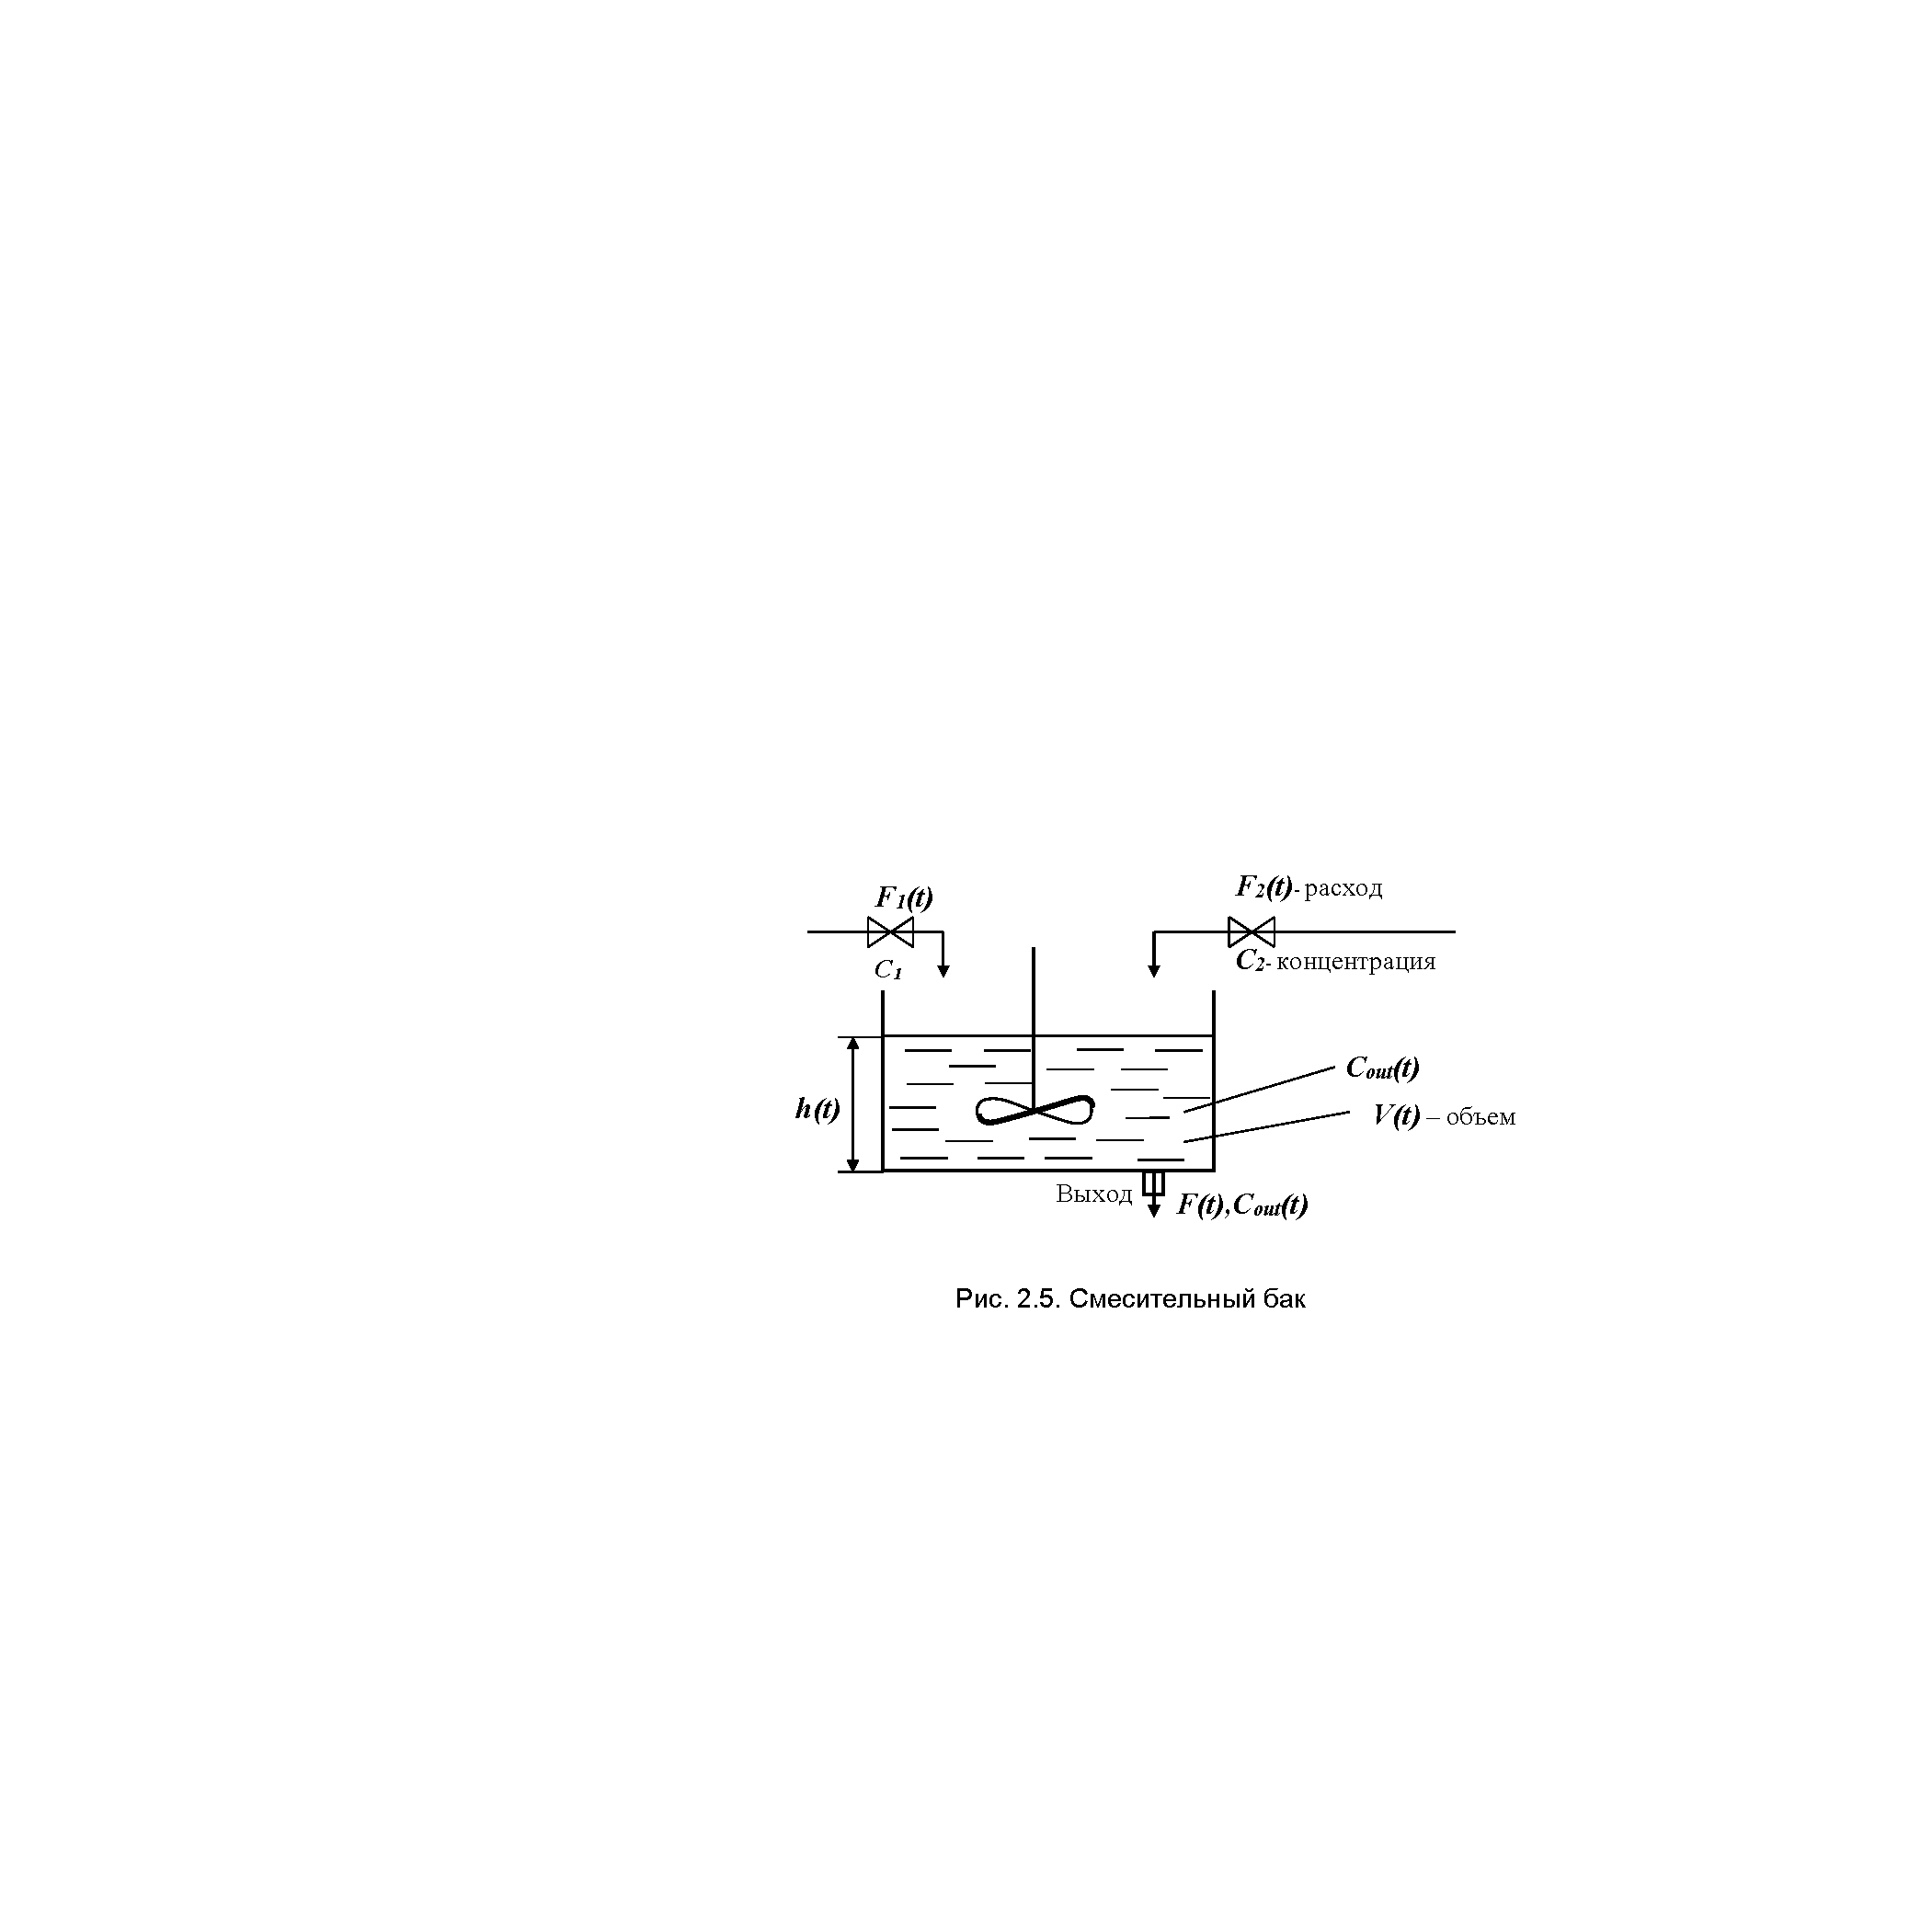
\includegraphics[width=14.526cm,height=8.555cm]{img-013}
	\caption{Смесительный бак}
	\label{fig:buc}
\end{figure}
\bigskip


		Мгновенный расход выходного потока при естественном истечении зависит от уровня жидкости в баке  $h(t)$ следующим
		образом:
\begin{equation}\label{eq:drain}
	F(t)=k\sqrt{h(t)}(2.2.11)
\end{equation}
		где   $k$ - некоторая константа. Это следует из уравнения Бернулли, которое описывает энергетический баланс жидкости
		перед сливным отверстием и после него. Потенциальная энергия жидкости перед сливным отверстием пропорциональна 
		$h$. При истечении из бака энергия жидкости превращается в кинетическую энергию потока, пропорциональную квадрату
		скорости  $\upsilon^2$. Приравнивая эти энергии, получаем  $\upsilon=k_{\upsilon}\sqrt h$. Расход  $F$ пропорционален произведению скорости
		истечения на площадь сливного отверстия, откуда и следует \eqref{eq:drain}%(2.2.11)
		.



		\ \ Если бак имеет постоянную по высоте площадь поперечного сечения  $S$, то

\begin{equation}\label{eq:buck}
 F(t)=k\sqrt{\frac{V(t)} S}. % (2.2.12)
\end{equation}
		Тогда из \eqref{eq:full mass} %(2.2.9) 
		и \eqref{eq:solute} %(2.2.10) 
		получаем
\begin{equation*}
\frac{\text{dV}(t)}{\text{dt}}=F_1(t)+F_2(t)-k\sqrt{\frac{V(t)} S},
\end{equation*}
\begin{equation*}
\frac
d{\text{dt}}\{C_{\text{out}}(t)V(t)\}=C_1F_1(t)+C_2F_2(t)-C_{\text{out}}(t)k\sqrt{\frac{V(t)}
	S}.
\end{equation*}

		Выберем в качестве базового режима \ установившееся состояние (статику), когда все величины являются постоянными - 
		$F_{10},F_{20},F_0,C_0,V_0$. При этом из предыдущих уравнений получаем
\begin{align*}
		&0=F_{10}+F_{20}-F_0,\\
		&0=C_1F_{10}+C_2F_{20}-C_0F_0.\\
		&F_0=k\sqrt{\frac{V_0} S}.
\end{align*}
		При известных $F_{10}$ и  $F_{20}$ эти уравнения могут быть разрешены относительно  $F_0,V_0$ и $C_0$:
		
\begin{equation*}
		F_0=F_{10}+F_{20};\quad V_0=S\frac{F_0^2}{K^2};\quad C_0=\frac{C_1F_{10}+C_2F_{20}}{F_0}.
\end{equation*}



		Предположим теперь, что возникли отклонения от установившегося состояния:
\begin{equation*}
		 F_1(t)=F_{10}+\Delta_1(t),
\end{equation*}
\begin{equation*}
	F_2(t)=F_{20}+Delta_2(t)
\end{equation*}
 и, как следствие,
\begin{align*}
	&F(t)=F_0+\Delta  (t),\\
	&V(t)=V_0+\Delta V(t)\;,\\
	&C_{\normalsubformula{\text{out}}}(t)=C_0+\Delta C(t)\;.
\end{align*}
		Если эти отклонения невелики, то можно провести линеаризацию нелинейных дифференциальных уравнений объекта.



		Сначала линеаризуем уравнение для полной массы
\begin{equation*}
\frac
d{{\text{dt}}}\{V_0+\mathit{\Delta  V}(t)\}=F_{10}+\mathit{\Delta  F}_1(t)+F_{20}+\mathit{\Delta  F}_2(t)-k\sqrt{\frac{V_0+\mathit{\Delta  V}(t)}
	S}.
\end{equation*}
		Используем разложение нелинейной функции в ряд Тейлора и учтём, что
%TODO понять что не так с формулой 
%\begin{equation*}
%	\frac d{\normalsubformula{\text{dV}}}\sqrt V\right\mid_{V=V_0}\cdot \Delta V_0=\frac 1 2\frac 1{\sqrt{V_0}}\Delta V.
%\end{equation*}
		Тогда
\begin{equation*}
\Delta \dot V(t)=F_{10}+\mathit{\Delta  }_1(t)+F_{20}+\mathit{\Delta  }_2(t)-k\sqrt{\frac{V_0} S}-\frac k{\sqrt S}\cdot
\frac{\mathit{\Delta V}(t)}{2\sqrt{V_0}}+R(t).
\end{equation*}
		Учитывая уравнение статики и пренебрегая остаточным членом, получим
\begin{equation}\label{eq:2.2.13}
		\Delta \dot V(t)=\mathit{\Delta  }_1(t)+\mathit{\Delta  }_2(t)-\frac k{2\sqrt{\normalsubformula{\text{SV}}_0}}\cdot
		\mathit{\Delta V}(t). %(2.2.13)
\end{equation}

		 Введём параметр  $\Theta=\frac{V_{0}}{F{0}}$, называемый временем заполнения бака. Тогда, учитывая \eqref{eq:buck} %(2.2.12)
		 , получим
\begin{equation}\label{key}
		  \frac k{2\sqrt{\text{SV}_{0}}}=\frac 1{2\Theta }.  %(2.2.14)
\end{equation}
		Кроме того, отметим, что 
\begin{equation}\label{key}
		  \frac{k\;\mathit{\Delta V}}{2\sqrt{\text{SV}_{0}}}=\frac{\mathit{\Delta V}}{2\Theta 
		  }=\mathit{\Delta F}.  %(2.2.15)
\end{equation}

	Таким образом, вместо \eqref{eq:2.2.13} %(2.2.13)
	 запишем

\begin{equation}\label{eq:2_2_16}
		 \Delta \dot V(t)=\mathit{\Delta}_{1}(t)+\mathit{\Delta  }_{2}(t)-\frac {1}{2\Theta }\cdot \mathit{\Delta V}(t). (2.2.16)
\end{equation}


		Проведем аналогичные действия для уравнения баланса масс растворённого вещества. 
\begin{align*}
&\frac
d{\text{dt}}\left\{\;\left[C_0+\mathit{\Delta C}(t)\right]\left[V_0+\mathit{\Delta V}(t)\right]\;\right\}=\\
&=C_1\left[F_{10}+\mathit{\Delta  }_1(t)\right]+C_2\left[F_{20}+\mathit{\Delta  }_2(t)\right]-\left[C_0+\mathit{\Delta C}(t)\right]k\sqrt{\frac{V_0+\mathit{\Delta V}(t)}
	S.}
\end{align*}
		После разложения в ряд Тейлора получим
\begin{align*}
&V_0\Delta \dot C(t)+C_0\Delta \dot V(t)=C_1F_{10}+C_1\mathit{\Delta  }_1(t)+C_2F_{20}+C_2\mathit{\Delta}_2(t)-
\\&-C_0k\sqrt{\frac{V_0} S}-k\sqrt{\frac{V_0} S}\mathit{\Delta C}(t)-\frac{C_0k}{2\sqrt{V_0S}}\mathit{\Delta V}(t)-R(t).
\end{align*}

		Учтём уравнения статики и отбросим \ остаточный член:
\begin{equation*}
\begin{matrix}V_0\Delta \dot C(t)+C_0\Delta \dot V(t)=C_1\mathit{\Delta  }_1(t)+C_2\mathit{\Delta  }_2(t)-\hfill\null \\-k\sqrt{\frac{V_0}
	S}\mathit{\Delta C}(t)-C_0\frac k{2V_0}\sqrt{\frac{V_0} S}\mathit{\Delta V}(t).\hfill\null \end{matrix}\hfill 
\end{equation*}
		Подставим в это уравнение  $\Delta \dot V(t)$ из \eqref{eq:2_2_16}%2.2.16
		). Получим
\begin{align*}
&V_0\Delta \dot C=C_1\mathit{\Delta}_1(t)+C_2\mathit{\Delta}_2(t)-F_0\mathit{\Delta C}(t)-
\\&-C_0\mathit{\Delta  }_1(t)-C_0\mathit{\Delta}_2(t)\;.
\end{align*}

		Таким образом, в результате линеаризации мы получили систему следующих дифференциальных уравнений, которые описывают
		процессы в смесительном баке:
\begin{equation}
\begin{cases}\label{eq:smethitelbak}
	\Delta \dot{V}(t)=\Delta F_{2}(t)+\Delta F_{2}(t)-\cfrac{1}{2\Theta}\Delta V(t),\\
	\Delta \dot{C}=-\cfrac{1}{\Theta}\Delta C(t)+\cfrac{C_{1}-C_{0}}{V_{0}}\Delta F_{1}(t)+\cfrac{C_{2}-C_{0}}{V_{0}}\Delta F_{2}t.
	 %(2.2.17)
\end{cases}
\end{equation}


		 На этом завершён для данного примера первый этап разработки - составлено математическое описание объекта и в
		результате линеаризации получена его линейная модель. Далее это описание нужно представить в удобной форме \ - в виде
		векторно-матричных дифференциальных уравнений и в виде структурной схемы.



	 Представим математическое описание объекта в виде векторно-матричных дифференциальных уравнений. Введем обозначения:



\begin{equation*}
		\vec x(t)=\left[\begin{matrix}\mathit{\Delta V}(t)\\\mathit{\Delta C}(t)\end{matrix}\right]\;\;; \  \vec
		u(t)=\left[\begin{matrix}\mathit{\Delta  }_1(t)\\\mathit{\Delta  }_2(t)\end{matrix}\right]\;\;; \  \vec
		y(t)=\left[\begin{matrix}\mathit{\Delta  }\\\mathit{\Delta C}\\\mathit{\Delta V}\end{matrix}\right].
\end{equation*}
		Теперь систему уравнений \eqref{eq:smethitelbak} %(2.2.17) 
		можно записать в векторно-матричном виде:
\begin{align*}
&\vec{\dot x}(t)=A\vec x(t)+B\vec u(t)\\
&\vec y(t)=C\vec x(t),
\end{align*}
		где
\begin{equation*}
		A=\left[\begin{matrix}-\cfrac 1{2\Theta }&0\\0&-\cfrac 1 \Theta \end{matrix}\right]; \ 
		B=\left[\begin{matrix}1&1\\\cfrac{C_1-C_0}{V_0}&\cfrac{C_2-C_0}{V_0}\end{matrix}\right]; \ 
		C=\left[\begin{matrix}\cfrac 1{2\Theta }&0\\0&1\\1&0\end{matrix}\right].
\end{equation*}
\bigskip
Структурная схема объекта представлена на рис.\ref{fig:2_6}.
%2.6. 
%TODO кадрировать
\begin{figure}[h]
	\centering
	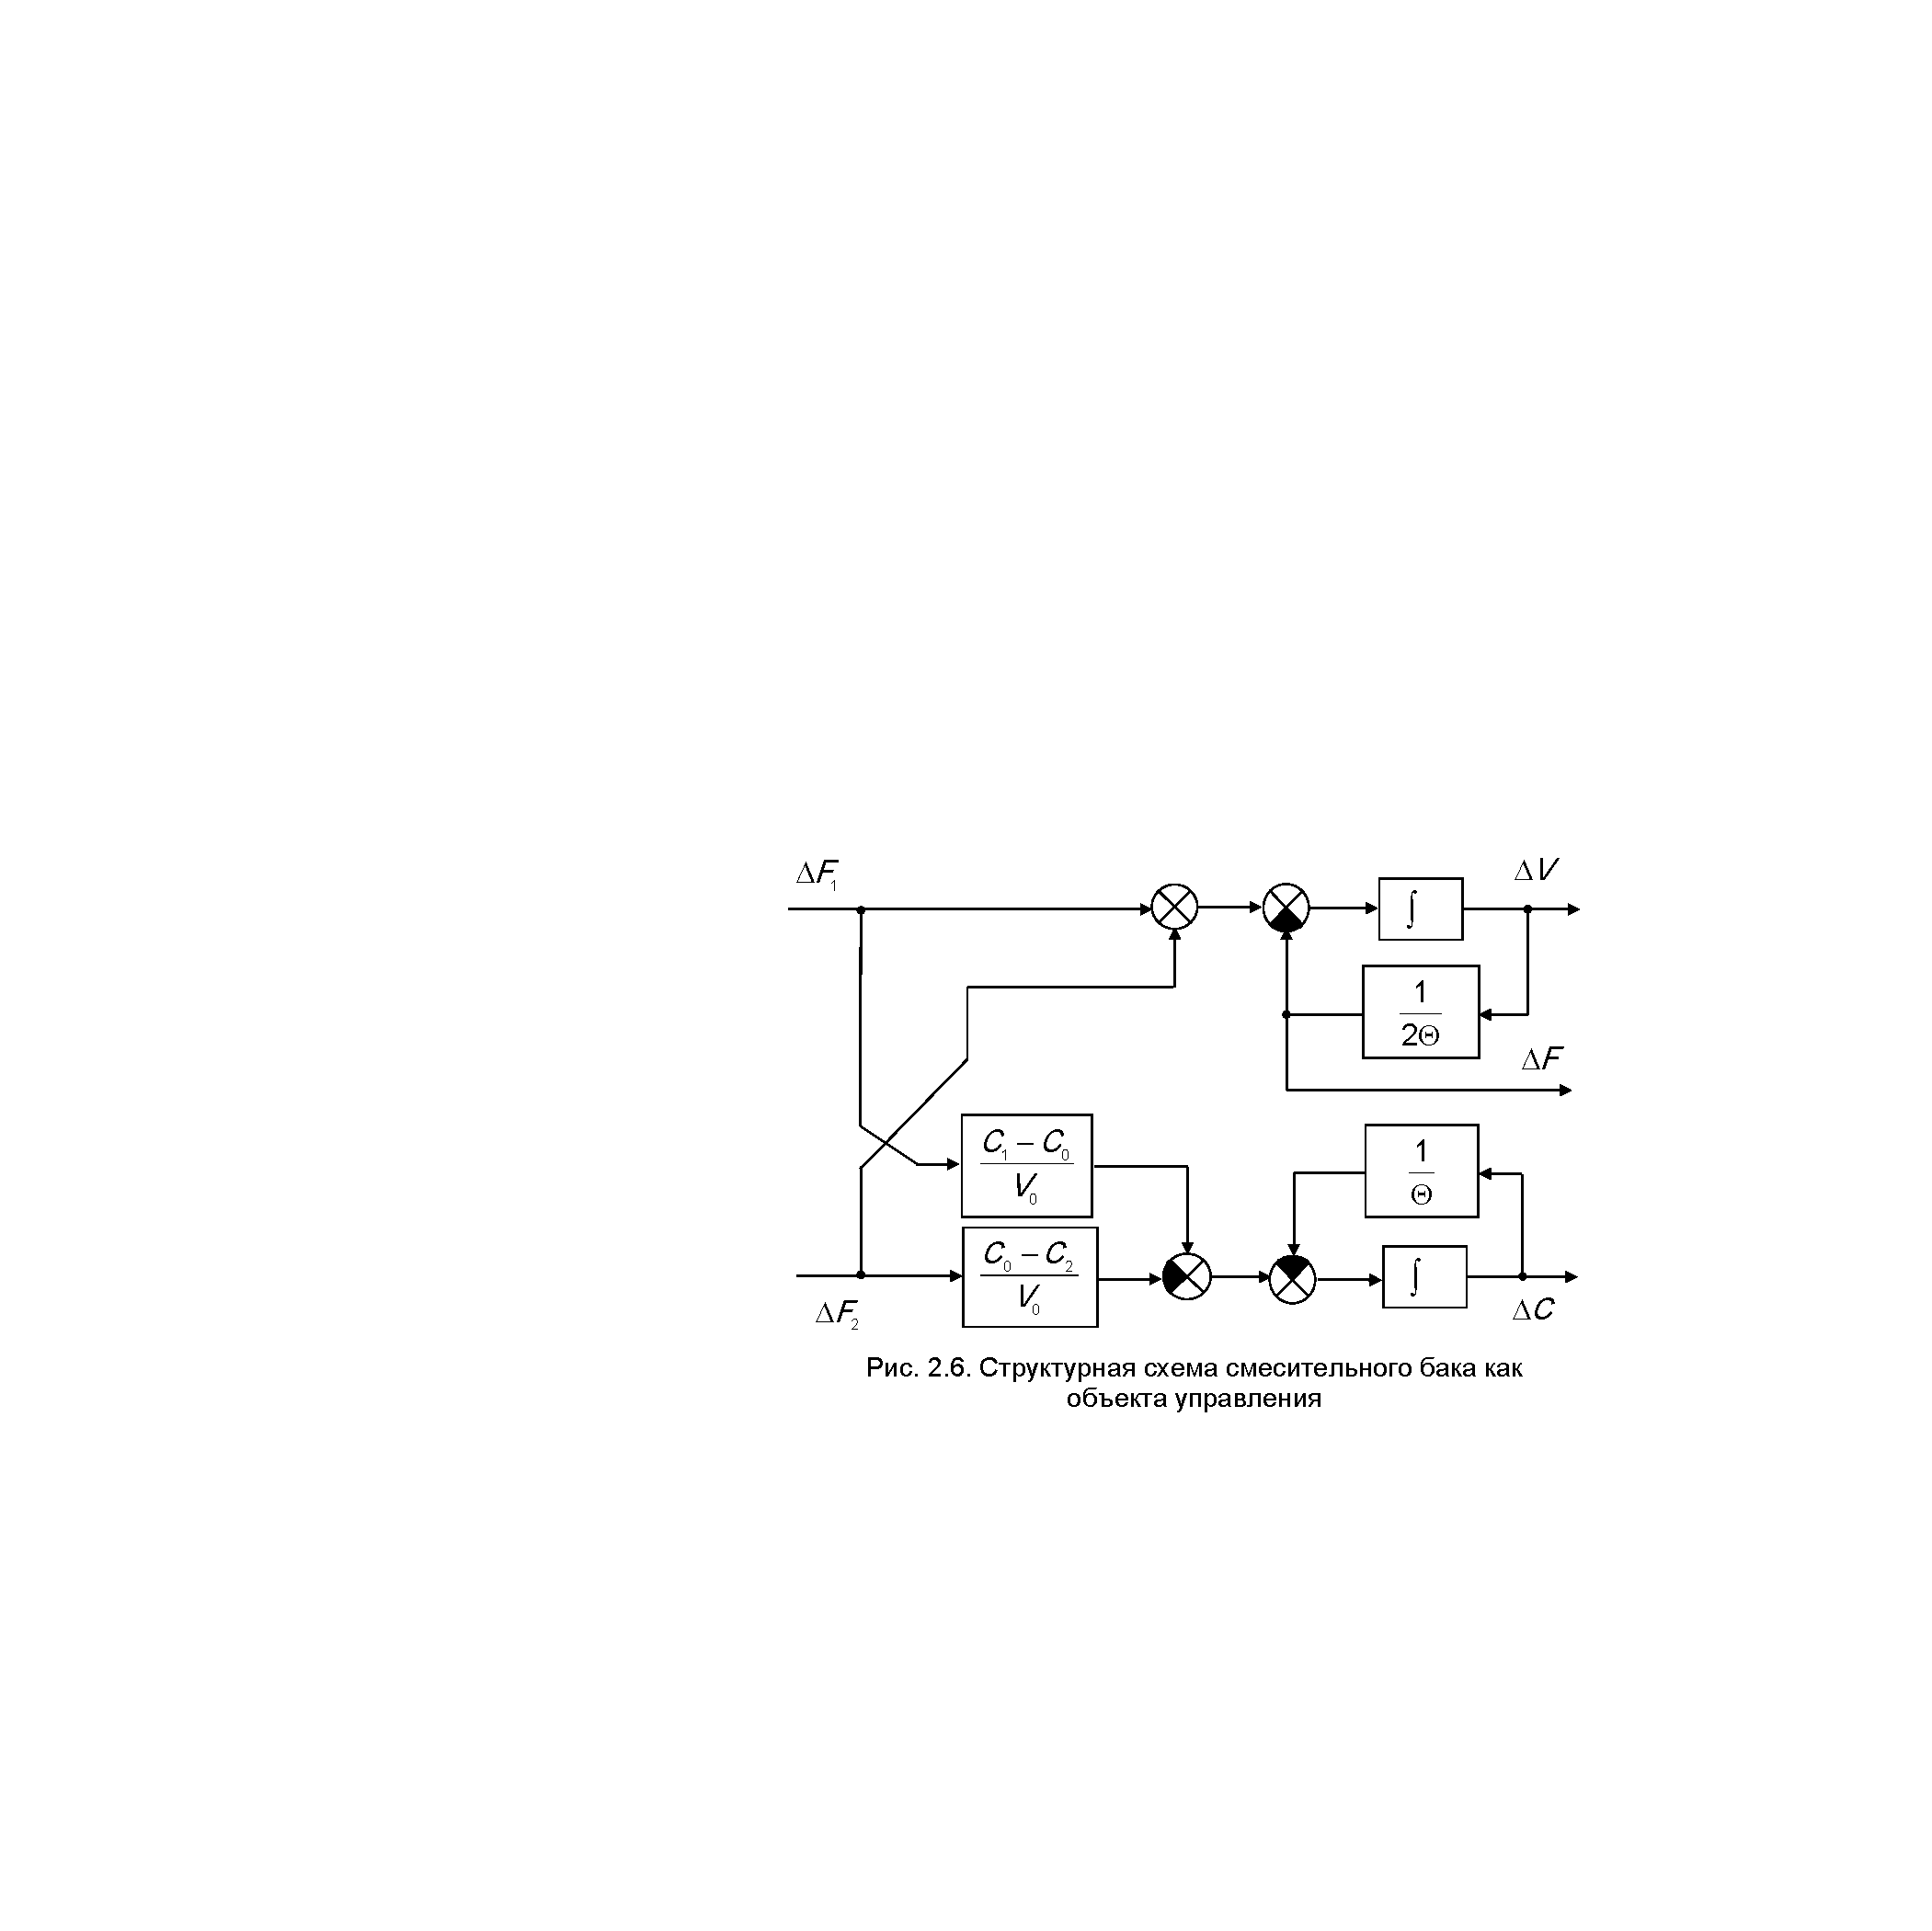
\includegraphics[width=14.975cm,height=10.689cm]{img-014} 
	\caption{Структурная схема смесительного бака как объекта управления}
	\label{fig:2_6}
\end{figure}
 %



\bigskip


		На основании полученных  дифференциальных уравнений и структурной схемы можно провести предварительный анализ
		свойств объекта и сделать следующие выводы.



		1. Изменение любой из входных переменных $\mathit{\Delta F}_1$ и $ \mathit{\Delta F}_{2} $ приводит к одновременному изменению всех выходных
		переменных  $\mathit{\Delta V}$,  $\mathit{\Delta  F}$ и  $\mathit{\Delta C}$. Это особенно наглядно следует из наличия перекрёстных
		связей на структурной схеме объекта.



		2. При ступенчатом изменении любой из входных переменных каждая из выходных переменных изменяется по экспоненциальному
		закону, причём темп изменения концентрации $\mathit{\Delta C}$ вдвое медленнее темпа изменения объёма  $\mathit{\Delta V}$.


		 Предметом отдельного рассмотрения при проектировании системы управления (СУ) должен стать анализ диапазонов
		изменения переменных объекта, в которых сохраняется адекватность линейной модели.


		 Прежде, чем закончить рассмотрение данного примера, имеет смысл продемонстрировать некоторые последующие действия
		разработчика в части синтеза алгоритмов управления. Перед разработчиком среди прочих встанут следующие две задачи. Одна
		из них - обеспечение заданных требований по длительности и качеству процессов в системе, то есть её динамических
		свойств. Рассмотрению соответствующих вопросов посвящён третий раздел настоящего пособия.



		Вторая задача - обеспечение возможности независимого управления объёмом (расходом) и концентрацией. Введём понятие
		командных сигналов по требуемым концентрации - $ \Delta r_{c} $ и объёму - 
		$\Delta r_{v}$. В статике производные всех переменных должны быть равны нулю и, как следует из структурной схемы и
		дифференциальных уравнений объекта, должны выполняться равенства


\begin{equation*}
		\mathit{\Delta  F}_{1}+\mathit{\Delta  F}_{2}-\frac 1{2\Theta }\cdot \mathit{\Delta V}_{\text{уст}}=0;
\end{equation*}
\begin{equation*}
		-\frac 1
		\Theta \mathit{\Delta C}_{\normalsubformula{\text{уст}}}+\frac{C_1-C_0}{V_0}\mathit{\Delta  }_1-\frac{C_0-C_2}{V_0}\mathit{\Delta  }_2=0.
\end{equation*}
		Отсюда, с учётом равенства  $\Theta =\cfrac{V_0}{F_0}$, получаем\ \ 
\begin{align}\label{eq:vus}
		&\mathit{\Delta V}_{\normalsubformula{\text{уст}}}=2\Theta (\mathit{\Delta  }_1+\mathit{\Delta  }_2);\ \\\ 
		%(2.2.18)
\label{eq:cust}
		&\mathit{\Delta C}_{\normalsubformula{\text{уст}}}=\frac{C_1-C_0}{F_0}\mathit{\Delta  }_1-\frac{C_0-C_2}{F_0}\mathit{\Delta  }_2.\ \ 
		%(2.2.19)
\end{align}

		Для компенсации перекрёстных связей в объекте введём перекрёстные связи в регуляторе:
\begin{align*}
		&\mathit{\Delta }_1=a_{\normalsubformula{\text{VF}}1}\mathit{\Delta r}_V+a_{\normalsubformula{\text{CF}}1}\mathit{\Delta r}_C;\\
		&\mathit{\Delta}_2=a_{\normalsubformula{\text{VF}}2}\mathit{\Delta r}_V+a_{\normalsubformula{\text{CF}}2}\mathit{\Delta r}_C.
\end{align*}
%TODO буква a имеет не тот вид, что делать 
		Подставим эти выражения в \eqref{eq:vus} %(2.2.18) 
		и \eqref{eq:cust} %(2.2.19)
		:
\begin{equation}\label{eq:2_2_20}
		\mathit{\Delta V}_{\normalsubformula{\text{уст}}}=2\Theta ((a_{\normalsubformula{\text{VF}}1}+a_{\normalsubformula{\text{VF}}2})\mathit{\Delta r}_V+(a_{\normalsubformula{\text{CF}}1}+a_{\normalsubformula{\text{CF}}2})\mathit{\Delta r}_C);
		 %(2.2.20)
\end{equation}

	\begin{align}\label{eq:2_2_21}
		\mathit{\Delta C}_{\normalsubformula{\text{уст}}}&=\left(\frac{С_1-С_0}{F_0}a_{\normalsubformula{\text{VF}}1}-\frac{С_0-С_2}{F_0}a_{{VF}2}\right)\mathit{\Delta r}_V+\\&\nonumber
		+\left(\frac{С_1-С_0}{F_0}a_{\normalsubformula{\text{CF}}1}-\frac{С_0-С_2}{F_0}a_{\normalsubformula{\text{CF}}2}\right)\mathit{\Delta r}_C
		 %(2.2.21)
	\end{align}



		Для того чтобы установившееся значение объёма жидкости в баке  $\mathit{\Delta V}_{\normalsubformula{\text{уст}}}$
		определялось только командным сигналом  $\mathit{\Delta r}_V$ и не зависело от  $\mathit{\Delta r}_C$, а выходная концентрация 
		$\mathit{\Delta C}_{\normalsubformula{\text{уст}}}$ определялась только командным сигналом  $\mathit{\Delta r}_C$ и не зависела от 
		$\mathit{\Delta r}_V$, в равенстве \eqref{eq:2_2_20} %(2.2.20)
		приравняем к нулю коэффициент при  $\mathit{\Delta r}_C$, а коэффициент при 
		$\mathit{\Delta r}_V$ приравняем к единице. В равенстве \eqref{eq:2_2_21} %(2.2.21) 
		приравняем к нулю коэффициент при  $\mathit{\Delta r}_V$, а
		коэффициент при  $\mathit{\Delta r}_C$ приравняем к единице. \ В результате решения получившейся системы уравнений получим



%\begin{equation}\label{key}
%		\begin{matrix}a_{\normalsubformula{\text{VF}}1}=\frac
%		1{2\Theta }\frac{C_0-C_2}{C_1-C_2}\;;\;\;\;\;a_{\normalsubformula{\text{VF}}2}=\frac
%		1{2\Theta }\frac{C_1-C_0}{C_1-C}\;;\;\hfill\null
%		\\a_{\normalsubformula{\text{CF}}1}=\frac{F_0}{C_1-C_2}\;\;;\;\;\;\;\;\;\;\;\;a_{\normalsubformula{\text{CF}}2}=-\frac{F_0}{C_1-C_2}\;\;\;\;.\;\;\;\hfill\null
%		\end{matrix}\hfill {\ \ }(2.2.22)
%\end{equation}

\begin{align}
&a_{VF1}=\frac1{2\Theta }\frac{C_0-C_2}{C_1-C_2};&a_{FV2}=\frac
1{2\Theta }\frac{C_1-C_0}{C_1-C_2}\\\nonumber
&a_{CF1}==\frac{F_0}{C_1-C_2};&a_{CF2}=-\frac{F_0}{C_1-C_2}
%(2.2.22)
\end{align}


		В итоге получаем представленную на рис.\ref{fig:buck_system} %2.7  
		структурную схему системы управления смесительным баком, в которой обеспечена
		развязка каналов. Последнее означает, что командный сигнал  $\mathit{\Delta r}_V$ влияет только на изменение объёма жидкости
		в баке, а командный сигнал  $\mathit{\Delta r}_C$ - только на изменение концентрации. Объём жидкости в баке связан с расходом
		выходного потока  $\mathit{\Delta  }$ коэффициентом пропорциональности  $2\Theta $, поэтому регулирование первого можно
		рассматривать как регулирование второго.

\begin{figure}[]
	\centering
	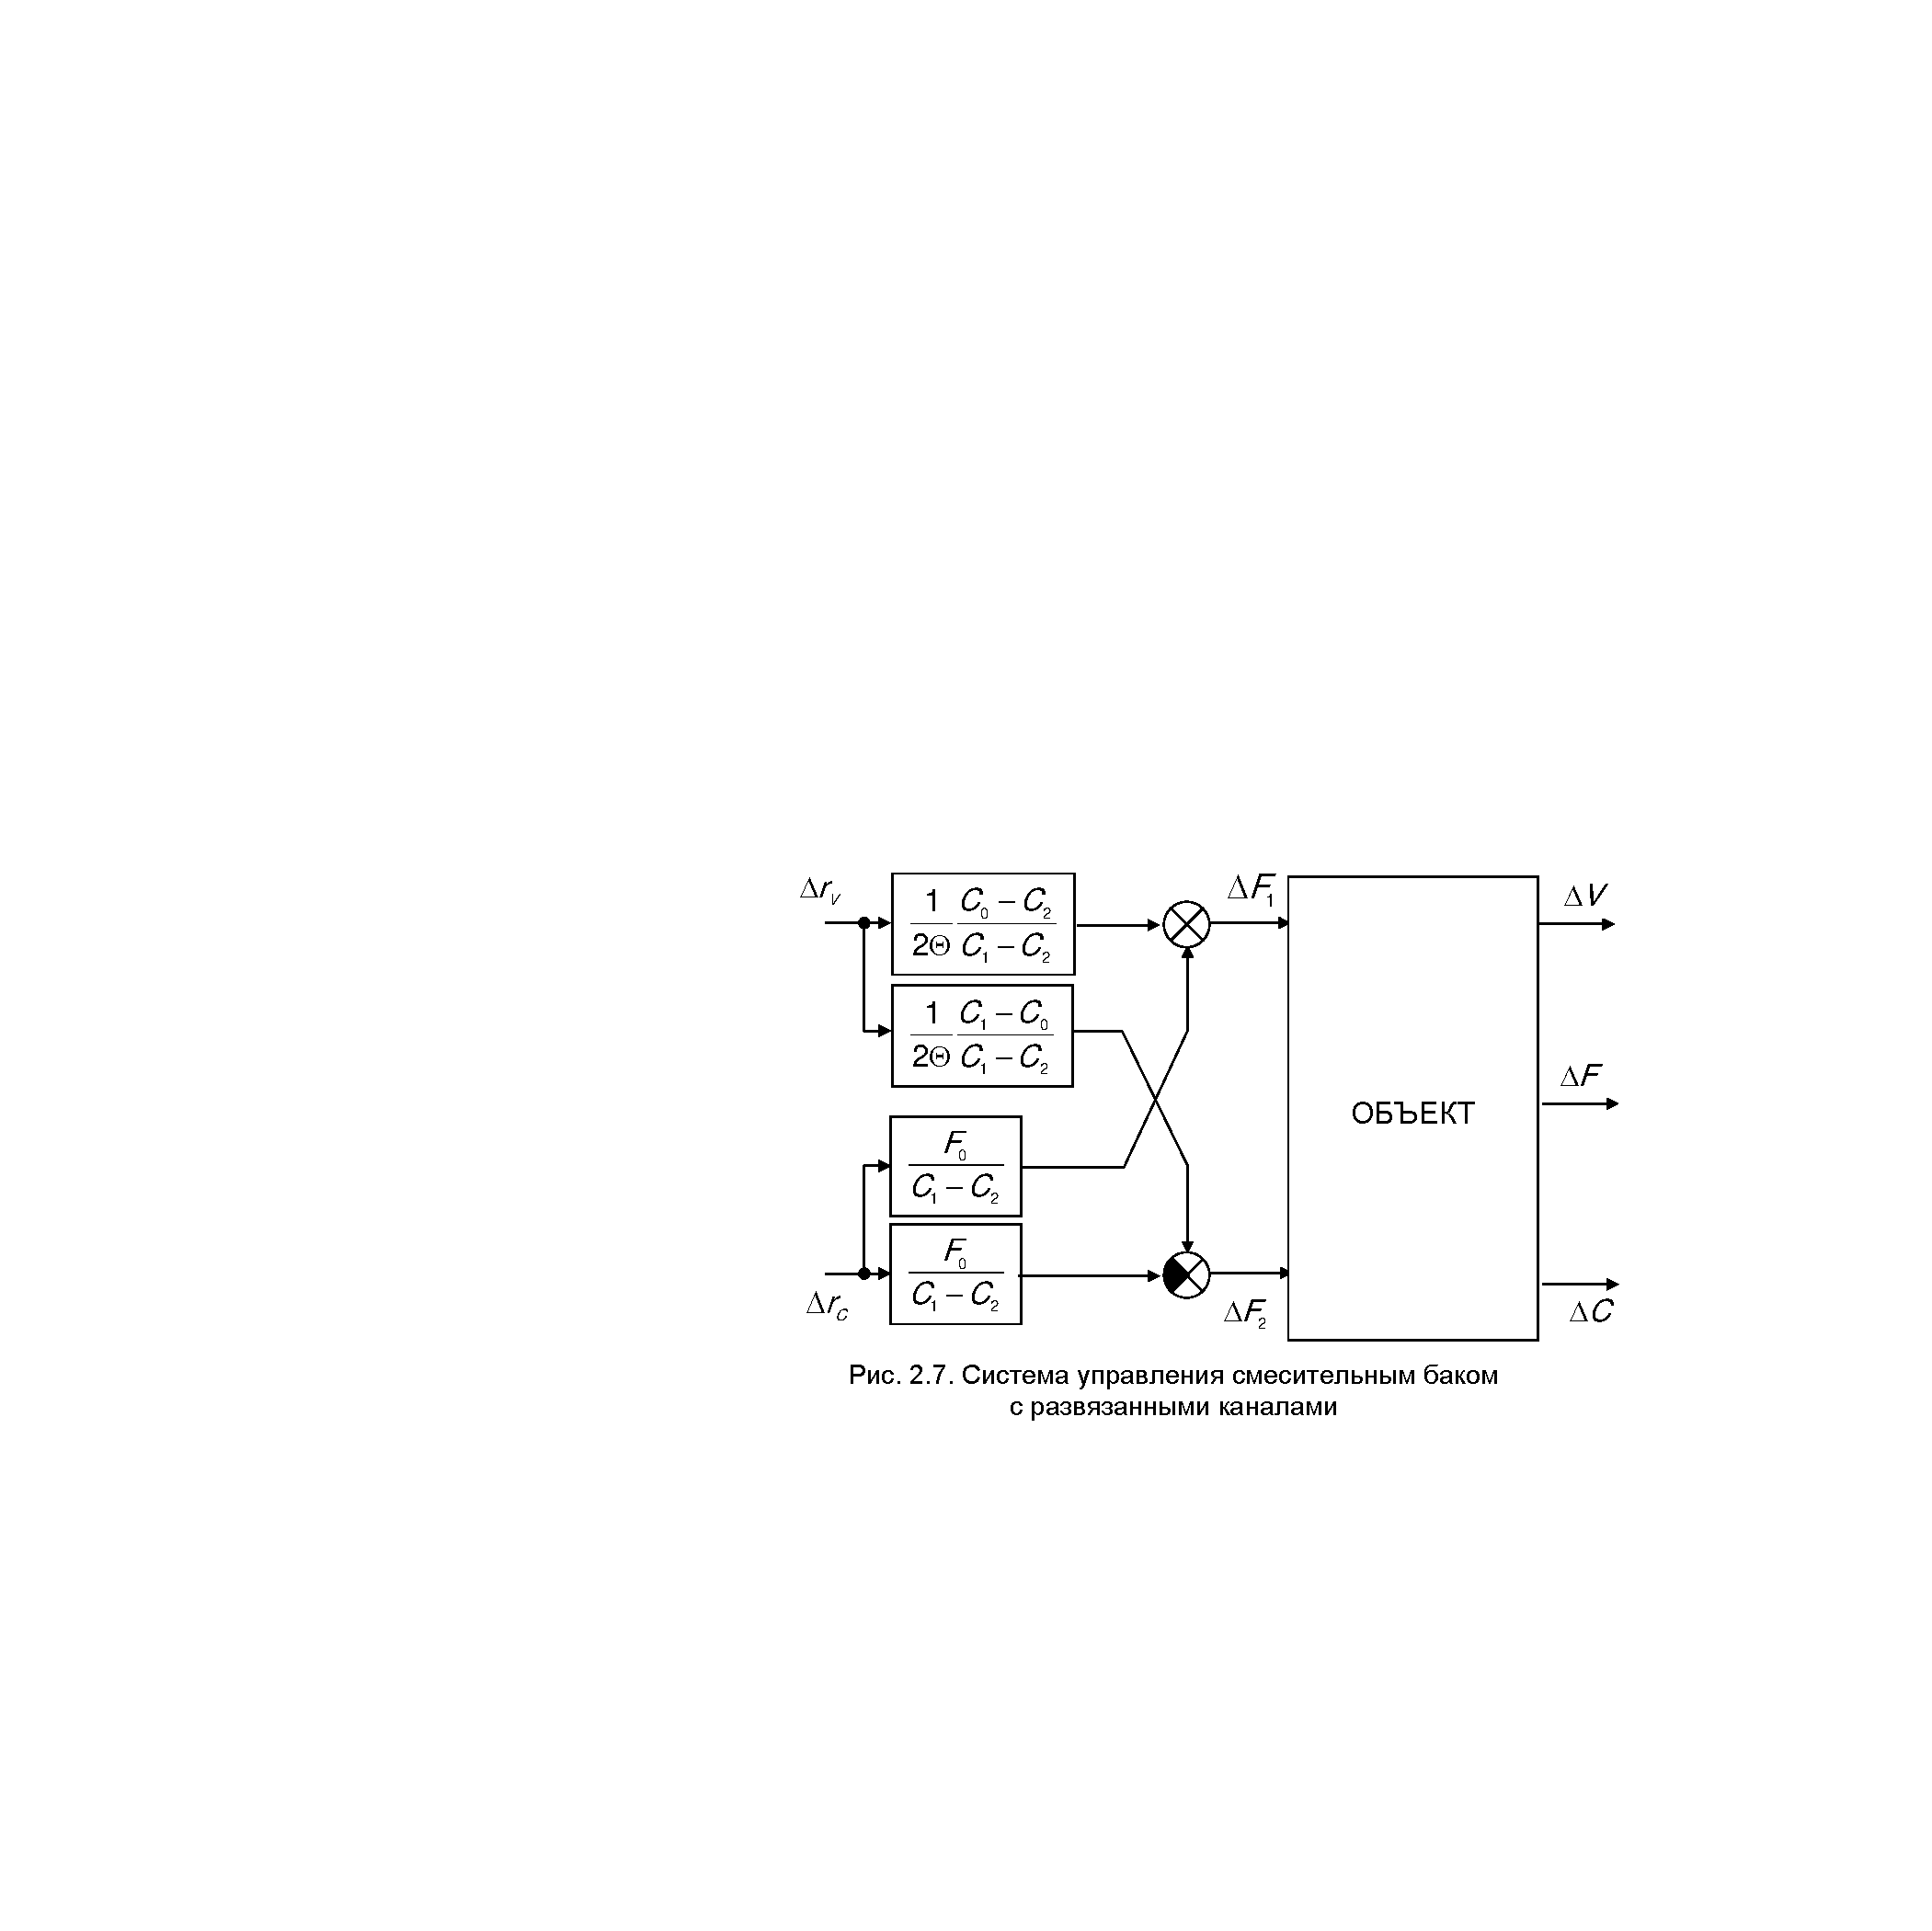
\includegraphics[width=15.849cm,height=10.61cm]{img-016}
	\caption{Система управления смесительным баком
		с развязанными каналами}
	\label{fig:buck_system} 
\end{figure}
\section{Линейные системы, заданные обыкновенными   дифференциальными уравнениями в нормальной форме Коши}
\subsection{Однородные дифференциальные уравнения}
		Рассмотрим прежде всего решение однородного векторно-матричного дифференциального уравнения
	\begin{equation}\label{eq:2_3_1}
	\vec{\dot x}(t)=A(t)\vec x(t),  (2.3.1)
	\end{equation}
		где каждому начальному условию  $\vec x(t_0)$ соответствует одно и только одно решение дифференциального уравнения.
		Будем полагать, что матрица  $A(t)$ непрерывна на промежутке  $t\in [0,\;\;\infty ]$. Множество всех решений образует
		{n}-мерное векторное пространство. Среди множества решений всегда может быть выбрано {n}
		линейно независимых.



		Это может быть сделано следующим образом. Зададим начальные условия  $\vec x_i(t_0)$, где  $i=1,2,\ldots,n$,
		совпадающие с базисными векторами  $\vec e_i$ пространства  $R^n$, то есть  $\vec x_i(t_0)=\vec e_i$. Из свойства
		единственности решений дифференциальных уравнений (через любую точку пространства состояний проходит одна и только одна
		траектория) следует линейная независимость решений с указанными начальными условиями. Матрица  $X(t)_{\left[n\times
			n\right]}$, столбцами которой являются  $n$ линейно независимых решений системы \eqref{eq:2_3_1}%(2.3.1)
		, называется фундаментальной
		матрицей этой системы дифференциальных уравнений.



		Поскольку каждый столбец фундаментальной матрицы является решением системы \eqref{eq:2_3_1}%(2.3.1)
		, то фундаментальная матрица
		удовлетворяет уравнению
\begin{equation}\label{eq:2_3_2}
		\dot X(t)=A(t)\cdot X(t), \text{ при начальных условиях }  X_0=X(t_0). (2.3.2)
\end{equation}
		По определению в любой момент времени столбцы этой матрицы линейно независимы, значит, ее определитель (определитель
		Вронского) не равен нулю на промежутке  $t\in [0,\infty ]$. Так как определитель матрицы  $X$ не равен нулю, то
		существует обратная матрица  $X^{-1}(t)$.


		Матрица
	\begin{equation}\label{eq:2_3_3}
	\Phi (t,t_0)=X(t)\cdot X^{-1}(t_0) 
	%(2.3.3)
	\end{equation}
		называется \textit{переходной матрицей} уравнения \eqref{eq:2_3_1} %(2.3.1)
		 или переходной матрицей, соответствующей матрице  $A(t)$.
		Переходная матрица является определяющей при анализе и решении дифференциальных уравнений и собственно в теории
		управления. Поэтому ниже приводятся основные её свойства, в основном непосредственно вытекающие из определения этой
		матрицы.

%TODO что делать с этим не знаю. Но судя по виду собирается нормально. Нумерация кривая !!!
\liststyleWWviiiNumxxvii
\begin{enumerate}
	\item 
			Переходная матрица при совпадающих значениях первого и второго аргумента становится единичной матрицей:
	
\end{enumerate}
		\ \  $\Phi (t,\;\;t_0)|_{t=t_0}=\Phi (t_0,\;\;t_0)=X(t_0)\cdot X^{-1}(t_0)=E$.


\liststyleWWviiiNumxxvii
\setcounter{saveenum}{\value{enumi}}
\begin{enumerate}
	\setcounter{enumi}{\value{saveenum}}
	\item 
			При любых значениях аргументов  $t_1,\;\;t_2$ переходная матрица  $\Phi (t_1,t_2)$ не вырождена и её определитель \ не равен
			нулю:
	
\end{enumerate}

		   $|\Phi (t_1,\;t_2)|\neq 0$.

\liststyleWWviiiNumxxvii
\setcounter{saveenum}{\value{enumi}}
\begin{enumerate}
	\setcounter{enumi}{\value{saveenum}}
	\item 
			Обращение матрицы  $\Phi (t,t_0)$ эквивалентно изменению порядка аргументов исходной матрицы: 
	
\end{enumerate}

		\ \  $\Phi ^{-1}(t,t_0)=\left[X(t)\cdot X^{-1}(t_0)\right]^{-1}=X(t_0)\cdot X^{-1}(t)=\Phi (t_0,t)$.


\liststyleWWviiiNumxxvii
\setcounter{saveenum}{\value{enumi}}
\begin{enumerate}
	\setcounter{enumi}{\value{saveenum}}
	\item 
			В соответствии с \eqref{eq:2_3_3}%(2.3.3)
	
\end{enumerate}

		\ \  $\dot \Phi (t,t_0)=\dot X(t)\cdot X^{-1}(t_0)=A(t)\cdot X(t)\cdot X^{-1}(t_0)=A(t)\cdot \dot \Phi (t,t_0)$.



		Это означает, что переходная матрица может быть определена как решение матричного дифференциального уравнения:
\begin{equation}\label{eq:2_3_4}
	\dot \Phi (t,t_0)=A(t)\cdot \Phi (t,t_0),\quad \Phi (t_0,t_0)=E. %(2.3.4)
\end{equation}


\liststyleWWviiiNumxxvii
\setcounter{saveenum}{\value{enumi}}
\begin{enumerate}
	\setcounter{enumi}{\value{saveenum}}
	\item 
			Переходная матрица определяет решение однородного векторно-матричного дифференциального уравнения \eqref{eq:2_3_1}%(2.3.1)
			,
			удовлетворяющее начальному условию  $\vec x(t)|_{t=t_0}=\vec x(t_0)$:
	
\end{enumerate}
	\begin{equation}\label{eq:2_3_5}
		\vec x(t)=\Phi (t,t_0)\cdot \vec x(t_0).  (2.3.5)
	\end{equation}



		\ Это действительно так, ибо, во-первых, при  $t=t_0$



		\ \  $\Phi (t_0,t_0)\cdot \vec x(t_0)=\vec x(t_0)$,
		\ во-вторых, с учетом свойства (4): 
\begin{equation*}
		\frac d{\normalsubformula{\text{dt}}}\{\Phi (t,t_0)\vec x(t_0)\}=\dot \Phi (t,t_0)\vec x(t_0)=A(t)\Phi (t,t_0)\vec x(t_0)=A(t)\vec
		x(t).
\end{equation*}


\liststyleWWviiiNumxxvii
\setcounter{saveenum}{\value{enumi}}
\begin{enumerate}
	\setcounter{enumi}{\value{saveenum}}
	\item 
			Из предыдущего свойства следует один из способов определения переходной матрицы. Обозначим через  $\varphi _{i,j}(t,t_0)$
			элемент {i}-й строки и {j}-го столбца переходной матрицы и запишем равенство (2.3.5) в
			развернутом виде:
	
\end{enumerate}

%		\newline
		
		$\left[\begin{matrix}x_1(t)\\x_2(t)\\...\\x_i(t)\\...\\x_n(t)\end{matrix}\right]=\left[\begin{matrix}\varphi _{11}(t,t_0)&\varphi _{12}(t,t_0)&...&\varphi _{1j}(t,t_0)&...&\varphi _{1n}(t,t_0)\\\varphi _{21}(t,t_0)&\varphi _{22}(t,t_0)&...&\varphi _{2j}(t,t_0)&...&\varphi _{2n}(t,t_0)\\...&...&...&...&...&...\\\varphi _{\mathit{i1}}(t,t_0)&\varphi _{\mathit{i2}}(t,t_0)&...&\varphi _{\normalsubformula{\text{ij}}}(t,t_0)&...&\varphi _{\normalsubformula{\text{in}}}(t,t_0)\\...&...&...&...&...&...\\\varphi _{\mathit{n1}}(t,t_0)&\varphi _{\mathit{n2}}(t,t_0)&...&\varphi _{\text{nj}}(t,t_0)&...&\varphi _{\normalsubformula{\text{nn}}}(t,t_0)\end{matrix}\right]\cdot
		\left[\begin{matrix}x_1(t_0)\\x_2(t_0)\\...\\x_j(t_0)\\...\\x_n(t_0)\end{matrix}\right]$,
$ \varphi $


		откуда следует выражение для i-й координаты вектора состояния:
\begin{equation*}
x_i(t)=\varphi _{i,1}(t,t_0)x_1(t_0)+\ldots +\varphi _{i,j}(t,t_0)x_j(t_0)+\ldots +\varphi _{i,n}(t,t_0)x_n(t_0).
\end{equation*}


		Если положить начальные условия по всем координатам вектора состояния, кроме {\textrm{j}}-й, нулевыми, а по
		{\textrm{j}}-й - единичными, то есть
\begin{equation}\label{eq"2_3_6}
		x_k(t_0)=0 \text{ при }  k=1,2,\ldots,n\;;\;\;\;k\neq j  \text{ и }   x_j=1, %(2.3.6)
\end{equation}
		то элемент {i}-й строки и {j}-го столбца матрицы  $\Phi (t,t_0)$ можно определить как процесс по i-й
		координате вектора состояния:
		\begin{equation}\label{eq:2_3_7}
		\varphi _{i,j}(t,t_0)=x_i(t).  
		%(2.3.7)
		\end{equation}
%TODO закончил тут
\liststyleWWviiiNumlxviii
\begin{enumerate}
	\item 
			К переходной функции применимо правило композиции:
	
\end{enumerate}
		\begin{equation}\label{eq:2_3_8}
		\Phi (t_2,t_0)=\Phi (t_2,t_1)\cdot \Phi (t_1,t_0). 
		%(2.3.8)
		\end{equation}



		Действительно, решение уравнения \eqref{eq:2_3_1} %(2.3.1) 
		в момент {t}\textsubscript{1} при начальных условиях  $\vec x(t_0)$
		имеет вид


\begin{equation*}
\vec x(t_1)=\Phi (t_1,t_0)\vec x(t_0).
\end{equation*}

		Если теперь этот результат принять за новые начальные условия, то к моменту времени  $t_2$ будем иметь:


\begin{equation*}
\vec x(t_2)=\Phi (t_2,t_1)\vec x(t_1)=\Phi (t_2,t_1)\cdot \Phi (t_1,t_0)\vec x(t_0).
\end{equation*}
\liststyleWWviiiNumlxviii
\setcounter{saveenum}{\value{enumi}}
\begin{enumerate}
	\setcounter{enumi}{\value{saveenum}}
	\item 
			Переходная матрица может быть вычислена с помощью ряда Пеано, или матрицианта матрицы  $A$:
	
\end{enumerate}
\begin{equation*}
\Phi (t,t_0)=M(A)=E+Q(A)+Q(A\cdot Q(A))+Q(A\cdot Q(A\cdot Q(A)))+\ldots ,
\end{equation*}

		где


\begin{equation*}
Q(A)=\overset t{\underset{t_0}{\int }}A(\tau )\mathit{d\tau }.
\end{equation*}

		Для того чтобы получить этот результат, проинтегрируем дифференциальное уравнение \eqref{eq:2_3_1} %(2.3.1)
		:



		\ \  $\vec x(t)=\vec x(t_0)+\overset t{\underset{t_0}{\int }}A(\tau _1)\vec x(\tau _1)\mathit{d\tau }_1$.



		Теперь повторим эту процедуру многократно, учитывая, что


\begin{equation*}
\vec x(\tau _1)=\vec x(t_0)+\overset{\tau _1}{\underset{t_0}{\int }}A(\tau _2)\vec x(\tau _2)\mathit{d\tau }_2.
\end{equation*}

		Тогда получим


\begin{equation*}
\begin{matrix}\vec x(t)=\vec x(t_0)+\overset t{\underset{t_0}{\int }}A(\tau _1)\mathit{d\tau }_1\vec x(t_0)+\overset
t{\underset{t_0}{\int }}A(\tau _1)\overset{\tau _1}{\underset{t_0}{\int }}A(\tau _2)\mathit{d\tau }_2\mathit{d\tau }_1\vec
x(t_0)+\hfill\null \\+\overset t{\underset{t_0}{\int }}A(\tau _1)\overset{\tau _1}{\underset{t_0}{\int
}}A(\tau _2)\overset{\tau _2}{\underset{t_0}{\int }}A(\tau _3)d(\tau _3)d(\tau _2)d(\tau _1)\vec x(t_0)+...=\hfill\null \\=\{E+\overset
t{\underset{t_0}{\int }}A(\tau _1)\mathit{d\tau }_1+\overset t{\underset{t_0}{\int }}A(\tau _1)\overset{\tau _1}{\underset{t_0}{\int
}}A(\tau _2)\mathit{d\tau }_2\mathit{d\tau }_1+...\}\vec x(t_0)\hfill\null \end{matrix}\;.\hfill 
\end{equation*}

		Если объект – стационарный и матрица А состоит из постоянных и не зависящих от времени элементов, то матрициант матрицы
		А (или ряд Пеано) превращается в выражение для матричной экспоненты:



		$\begin{matrix}\Phi (t,t_0)=E+A(t-t_0)+\frac{A^2(t-t_0)^2}{2!}+\frac{A^3(t-t_0)^3}{3!}+...=\hfill\null
		\\=\text{exp}(A(t-t_0))=e^{A(t-t_0)}.\hfill\null \end{matrix}\hfill $\ \ (2.3.9)



		Очевидно, что в стационарном случае переходная матрица является уже функцией только одного аргумента, равного разности
		начального и текущего (конечного) времени:



		\ \  $\Phi (t,t_0)=\Phi (t-t_0)=e^{\mathit{A\Delta t}}.$\ \ (2.3.10)



		Переходная матрица для стационарного объекта обладает рядом дополнительных замечательных свойств, трансформирующихся из
		соответствующих свойств переходной матрицы для нестационарного   объекта :



		из 1) -  $\Phi (0)=E$;  (2.3.11)



		из 3) -  $\Phi ^{-1}(\mathit{\Delta t})=\Phi (-\mathit{\Delta t})=e^{-A\cdot \mathit{\Delta t}}$ ;\ \ (2.3.12)



		из 4) - 
%		$\frac{\normalsubformula{\text{d\Phi }}(t-t_0)}{\normalsubformula{\text{dt}}}=0+A+\frac{2A^2(t-t_0)}{2!}+\frac{3A^3(t-t_0)^2}{3!}+...=$



		$=A\cdot \Phi (t-t_0)=A\cdot e^{A(t-t_0)}=e^{A(t-t_0)}\cdot A\;$;\ \ (2.3.13)



		из 5) - решение однородного дифференциального уравнения имеет вид



		\ \  $\vec x(t)=e^{A(t-t_0)}\cdot \vec x(t_0)$;  (2.3.14)



		из 7) -  $\Phi (k\cdot \mathit{\Delta t})=\Phi ^k\cdot (\mathit{\Delta t})$.  (2.3.15)



\bigskip


\bigskip

\subsection{Решение неоднородных векторно-матричных дифференциальных уравнений}

		Ранее были получены выражения для определения решений однородного дифференциального уравнения нестационарной



		\ \  $\vec x(t)=\Phi (t,t_0)\cdot \vec x(t_0)$  (2.3.5)



		и стационарной 



		\ \  $\vec x(t)=e^{A(t-t_0)}\cdot \vec x(t_0)$  (2.3.16)



		систем. Используем эти результаты для определения решения неоднородного линейного векторно-матричного уравнения,
		соответствующего (2.2.7):



		\ \  $\vec{\dot x}=A(t)\cdot \vec x(t)+B(t)\cdot \vec u(t)\;$.\ \ (2.3.17)



		Произведем замену:



		\ \  $\vec x(t)=\Phi (t,t_0)\cdot \vec z(t)$  (2.3.18)



		и продифференцируем это выражение:


\begin{equation*}
\vec{\dot x}(t)=\dot \Phi (t,t_0)\cdot \vec z(t)+\Phi (t,t_0)\cdot \vec{\dot z}(t)=
\end{equation*}

		\ \     $=A(t)\cdot \Phi (t,t_0)\cdot \vec z(t)+\Phi (t,t_0)\cdot \vec{\dot z}(t)$.



		Сопоставляя это выражение с предыдущим, получим



		\ \  $\Phi (t,t_0)\cdot \vec{\dot z}(t)=B(t)\cdot \vec u(t)$,



		откуда



		\ \  $\vec{\dot z}(t)=\Phi (t_0,t)\cdot B(t)\cdot \vec u(t)$,



		или, интегрируя,



		\ \  $\vec z(t)=\vec z(t_0)+\overset t{\underset{t_0}{\int }}\Phi (t_0,\tau )B(\tau )\cdot \vec u(\tau )\mathit{d\tau }$.



		Из (2.3.18) видно, что 



		\ \  $\vec z(t_0)=\vec x(t_0)$. 



		В итоге получаем выражение для решения векторно-матричного линейного неоднородного дифферен­циального уравнения,
		известное под названием формулы Коши:



		\ \  $\vec x(t)=\Phi (t,t_0)\cdot \vec x(t_0)+\overset t{\underset{t_0}{\int }}\Phi (t,\tau )B(\tau )\vec u(\tau )\mathit{d\tau }$.\ \ (2.3.19)



\bigskip

\section{Некоторые сведения из теории матриц}
\subsection{Собственные числа, характеристический полином,
	  присоединенная матрица}
\hypertarget{RefHeadingToc455659702}{}
		Умножение квадратной матрицы  $A$ на некоторый вектор  $\vec x$ дает новый вектор  $\vec z$, который, в общем случае,
		иначе ориентирован в про­странстве и имеет другую длину по сравнению с исходным вектором. Однако существуют и такие
		векторы, которые при выполнении этой опе­рации меняют только свою длину, но не меняют направления, то есть



		\ \  $A\vec v=\lambda \vec v,$\ \ (2.4.1)



		где  $\lambda $ - вещественная или комплексная скалярная величина, назы­ваемая собственным значением (характеристическим
		числом) матрицы  $A$, а вектор  $\vec v$ - собственный вектор этой матрицы. В развёрну­том виде уравнение (2.4.1) имеет
		следующий вид:



		\ \  $\left\{\begin{matrix}a_{11}v_1+a_{12}v_1+\ldots +a_{1n}v_n=\mathit{\lambda v}_1\\a_{21}v_1+a_{22}v_1+\ldots
		+a_{2n}v_n=\mathit{\lambda v}_2\\\ldots \ldots \ldots \ldots \ldots \ldots \ldots \ldots \ldots \ldots \ldots \ldots \ldots
		\\a_{\mathit{n1}}v_1+a_{\mathit{n2}}v_1+\ldots
		+a_{\normalsubformula{\text{nn}}}v_n=\mathit{\lambda v}_n\end{matrix}\right.$.\ \ 



		Очевидно, что для существования ненулевых  $v_i$ необходимо вы­пол­не­ние условия



		\ \  $\text{det}(\mathit{\lambda E}-A)\equiv |\mathit{\lambda E}-A|=0$. \ \ (2.4.2)



		Это уравнение называют характеристическим, или вековым уравнением матрицы  $A$. Левая часть этого уравнения называется
		характеристичес­ким полиномом, степень его равна размеру {n} матрицы  $A$:



		\ \  $\varphi _A(\lambda )=|\mathit{\lambda E}-A|=\lambda ^n+\alpha _1\lambda ^{n-1}+\alpha _2\lambda ^{n-2}+\ldots +\alpha _{n-1}\lambda ^1+\alpha _n$.\ \ (2.4.3)



		Таким образом, каждая квадратная матрица  $A$ имеет  $n$ собственных зна­чений  $\lambda _{1,}\lambda _{2,}\ldots ,\lambda _{n,}$, которые
		могут быть определены путём решения характеристического уравнения с использованием стандартного матема­тического
		обеспечения на цифровых вычислительных машинах.



\bigskip


		Алгебраическая кратность корня  $\lambda $ – это его кратность как корня характеристического уравнения. Геометрическая
		кратность корня  $\lambda $ – это количество линейно независимых векторов  $\vec v$, связанных с   данным  $\lambda $.


$ \lambda  $
		Если  $\lambda $ не является собственным значением матрицы  $A$, то существует матрица$\textit(\mathit{\lambda  E}-A)^{-1}$. По
		правилу определения обратных матриц



		\ \  $(\mathit{\lambda  E}-A)^{-1}=\frac{I(\lambda )}{|\mathit{\lambda  E}-A|}$,\ \ (2.4.4)



		где  $I(\lambda )$\textrm{ - }присоединённая матрица для матрицы  $A$. Ее элементы определяются как алгебраические дополнения
		элементов матрицы  $(\mathit{\lambda  E}-A)^T$. Здесь символ Т означает транспонирование. \ Присоединённая матрица - это
		матричный полином степени {n}-1:



		\ \  $I(\lambda )=\mathit{E\lambda }^{n-1}+I_1\lambda ^{n-2}+\ldots +I_{n-2}\lambda +I_{n-1}$,\ \ (2.4.5)



		где \  $E$\textit{ }– единичная матрица  $\left[n\times n\right]$.



		Если все собственные числа матрицы  $A$ различны, то собственные векторы матрицы  $A$ могут быть выбраны
		пропорциональными любым ненулевым столбцам матрицы  $I(\lambda _i)\;,\;\;\;i=1\;,\;\;2\;,\;\;...\;,\;\;n$.



\bigskip


		ПРИМЕР 2.4.1. Пусть объект задан структурной схемой, приведённой \ \ на рис.2.8.



\bigskip
\begin{figure}[h]
	\centering
	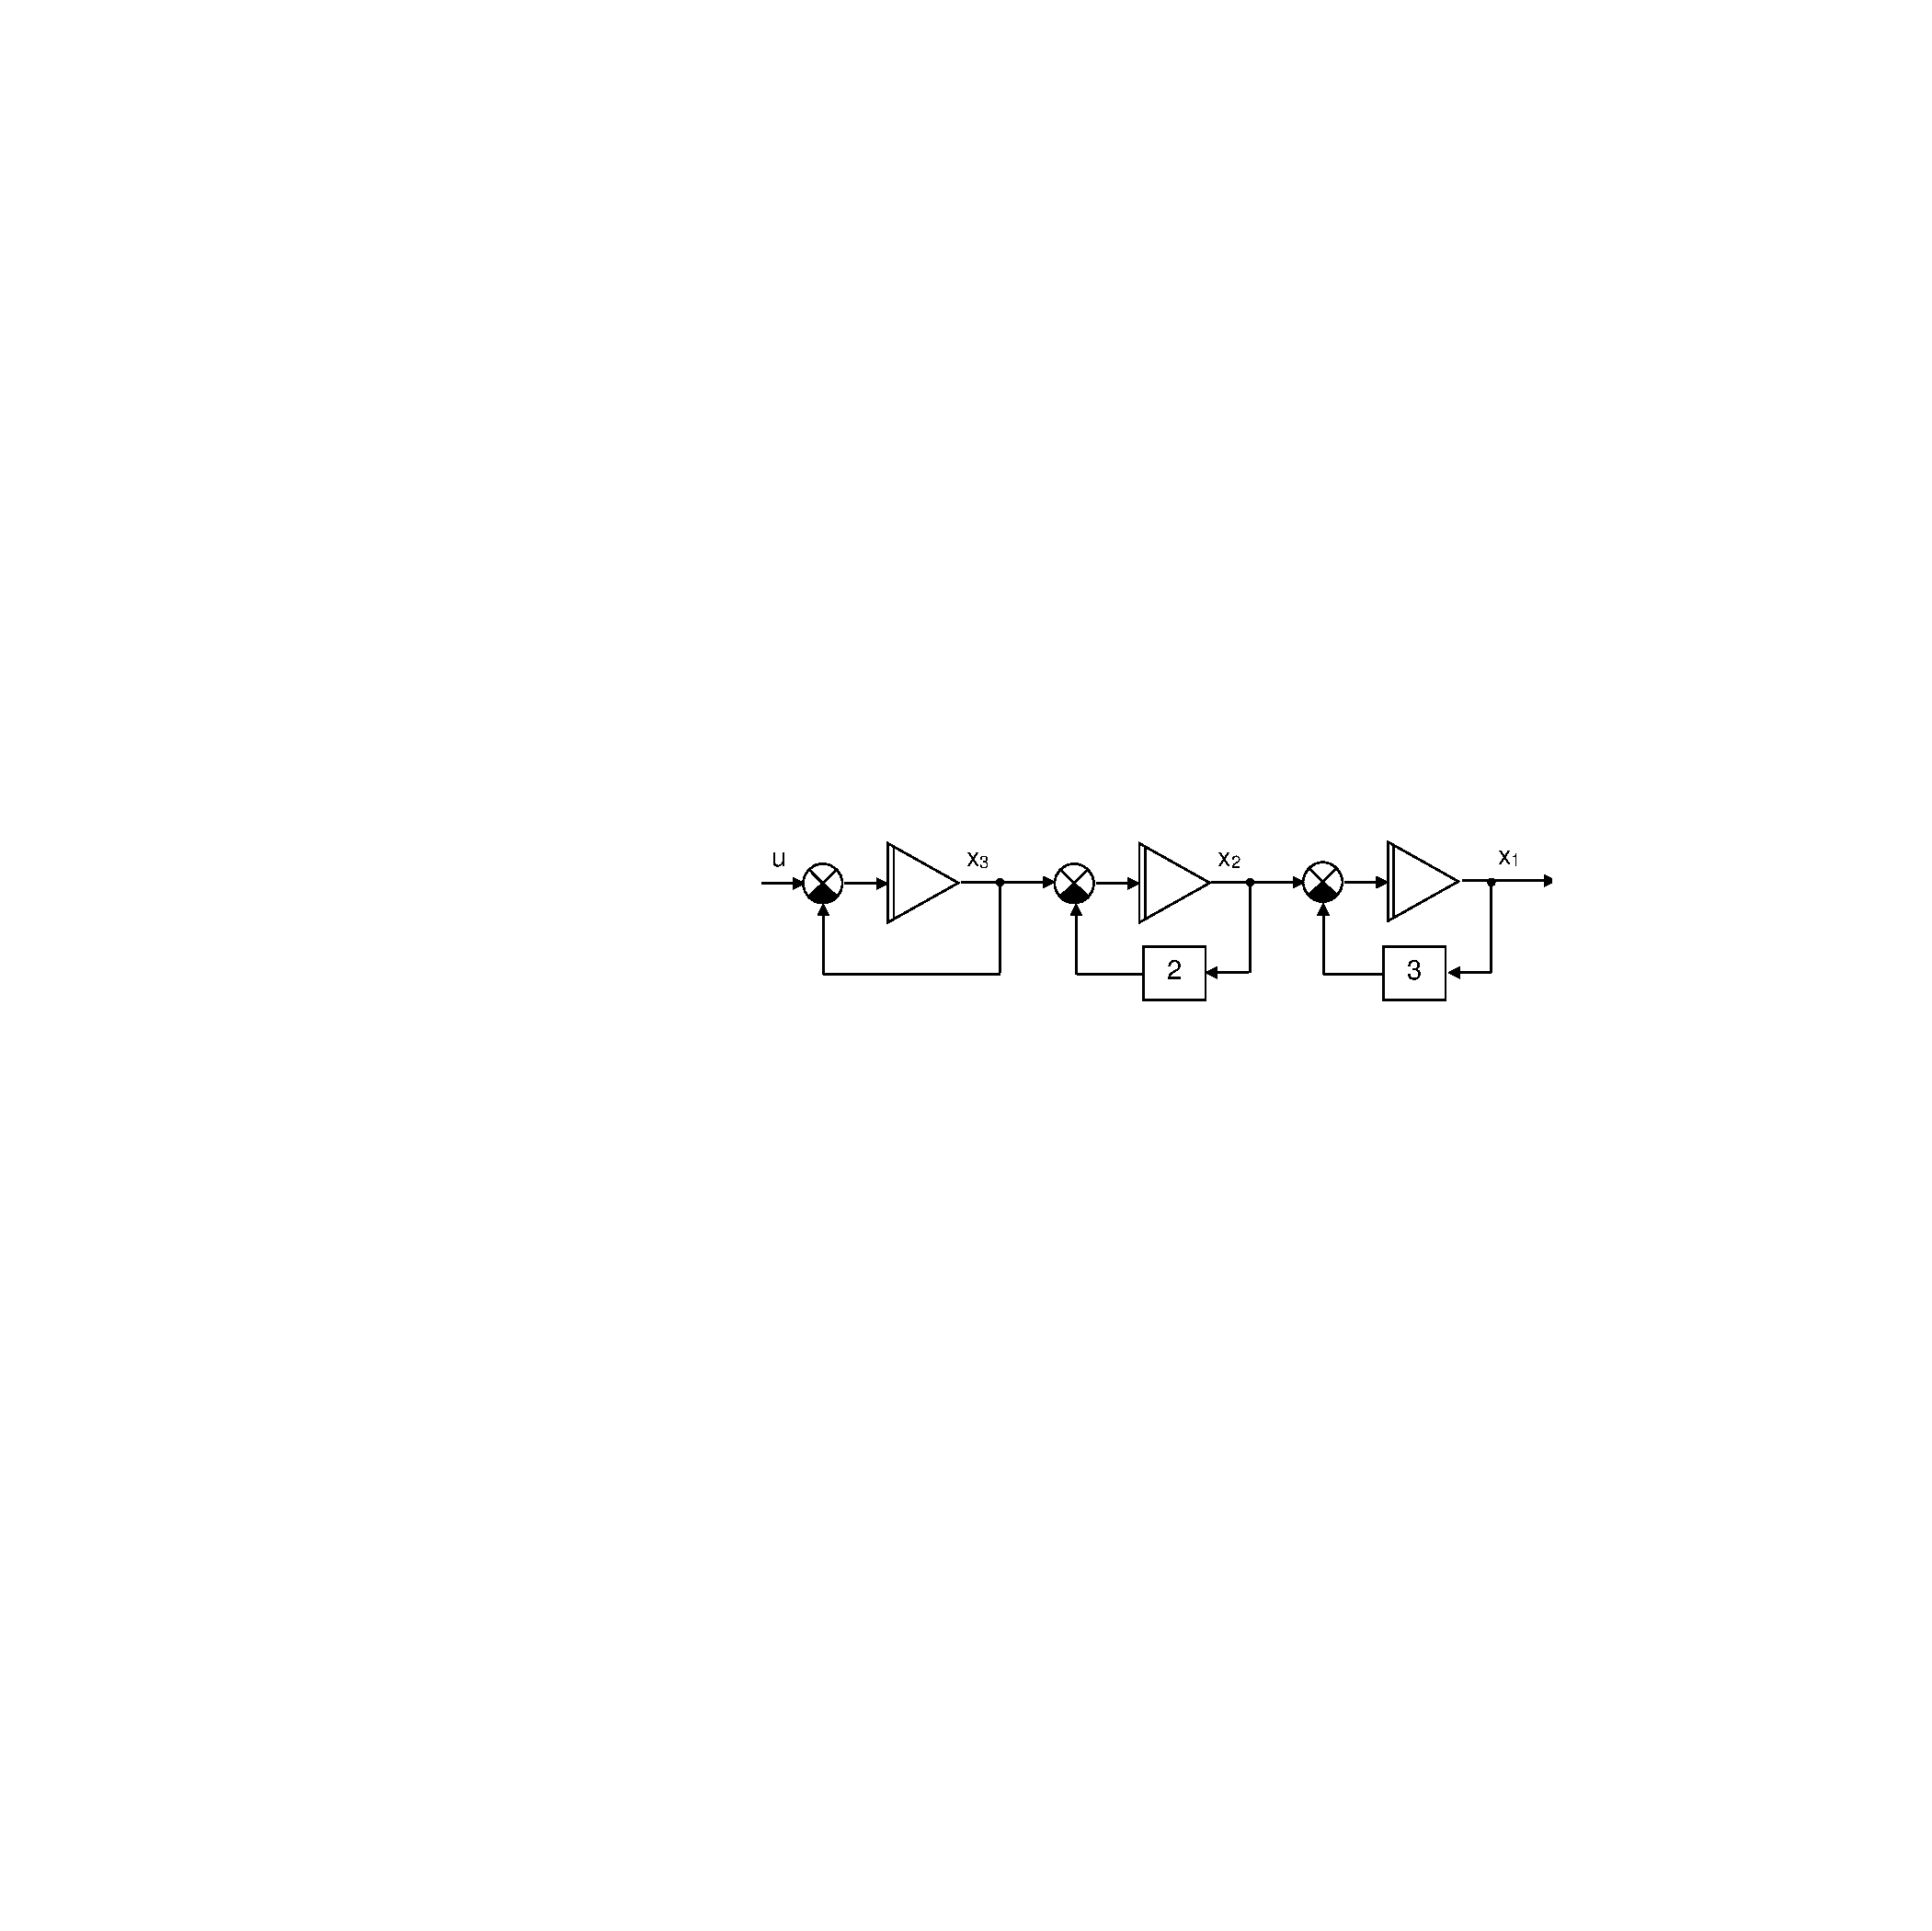
\includegraphics[width=14.79cm,height=4.366cm]{img-017}
	\caption {Структурная схема к примеру 2.4.1}
\end{figure}





		Ему соответствует система уравнений



		\ \  $\dot x_1=-3x_1+x_2$;



		\ \  $\dot x_2=-2x_2+x_3$;



		\ \  $\dot x_3=-x_3+u$,



		\ или в матричном виде 



		\ \  $\vec{\dot x}(t)=A\vec x(t)+\normalsubformula{\text{Bu}}(t)$,\ \ 



		где



		\ \  $A=\left[\begin{matrix}-3&1&0\\0&-2&1\\0&0&-1\end{matrix}\right]$; \ \ 
		$B=\left[\begin{matrix}0\\0\\1\end{matrix}\right]$.



		Для этих исходных данных получаем характеристический полином



		$\varphi _A(\lambda )=|\begin{matrix}\lambda +3&-1&0\\0&\lambda +2&-1\\0&0&\lambda +1\end{matrix}|=\lambda ^3+6\lambda ^2+11\lambda +6$.



		Ему соответствуют собственные числа


\begin{equation*}
\lambda _1=-1,^{}\lambda _2=-2,^{}\lambda _3=-3.
\end{equation*}

		Найдем присоединенную матрицу


\begin{equation*}
I(\lambda )=\left[\begin{matrix}(\lambda +2)(\lambda +1)&\lambda +1&1\\0&(\lambda +3)(\lambda +1)&\lambda +3\\0&0&(\lambda +3)(\lambda +2)\end{matrix}\right]=
\end{equation*}

		\ \ =
		$E_3\lambda ^2+\left[\begin{matrix}3&1&0\\0&4&1\\0&0&5\end{matrix}\right]\lambda +\left[\begin{matrix}2&1&1\\0&3&3\\0&0&6\end{matrix}\right].$



		Найдём собственные векторы матрицы  $A$:


\begin{equation*}
I(\lambda _1)=\left[\begin{matrix}0&0&1\\0&0&2\\0&0&2\end{matrix}\right];\;\;\;I(\lambda _2)=\left[\begin{matrix}0&-1&1\\0&-1&1\\0&0&0\end{matrix}\right];\;\;\;I(\lambda _3)=\left[\begin{matrix}2&-2&1\\0&0&0\\0&0&0\end{matrix}\right]
\end{equation*}

		и можно выбрать



		\ \  $\vec v_1=\left[\begin{matrix}1\\2\\2\end{matrix}\right];\;\;\;\;\;\vec
		v_2=\left[\begin{matrix}1\\1\\0\end{matrix}\right];\;\;\;\;\;\vec v_3=\left[\begin{matrix}1\\0\\0\end{matrix}\right]$.



		Полученный результат нетрудно проверить прямой подстановкой в (2.4.1).



		Имеется ряд алгоритмов для определения коэффициентов характеристического полинома и присоединенной матрицы. Один из
		наиболее употребимых - это \textbf{алгоритм $ \Phi $ аддеева - Леверье}. Он состоит в следующей последовательности вычислений:


\begin{equation*}
\begin{matrix}A_1=A;\ \ \ \alpha _1=-\normalsubformula{\text{SpA}}_1;\ \ \ I_1=A_1+\alpha _1E;\hfill\null
\\A_2=\normalsubformula{\text{AI}}_1;\ \ \alpha _2=-\frac 1 2\normalsubformula{\text{SpA}}_2;\ \ I_2=A_2+\alpha _2E;\hfill\null
\end{matrix}\hfill 
\end{equation*}

		. . . . . . . . . . . . . . . . . . . . . . . . . . . . . . . . . . . . . . . . . .


\begin{equation*}
\begin{matrix}A_{n-1}=\normalsubformula{\text{AI}}_{n-2};\ \ \ \alpha _{n-1}=-\frac
1{n-1}\normalsubformula{\text{SpA}}_{n-1};\ \ \ I_{n-1}=A_{n-1}+\alpha _{n-1}E;\hfill\null
\\A_n=\normalsubformula{\text{AI}}_{n-1};\ \ \alpha _n=-\frac 1
n\normalsubformula{\text{SpA}}_n;\ \ I_n=A_n+\alpha _nE=0.\hfill\null \end{matrix}\hfill 
\end{equation*}

		Здесь через  $\normalsubformula{\text{SpA}}$ обозначен след матрицы  $A$, то есть сумма ее диагональных элементов



		\ \  $\normalsubformula{\text{SpA}}=\overset n{\underset{i=1}{\sum }}a_{\normalsubformula{\text{ii}}}$.



		Последнее равенство процедуры используется для контроля точности вычислений.



		Для объекта, приведенного в примере 2.4.1,



		\ \ 
		$A_2=\left[\begin{matrix}-9&1&1\\0&-8&3\\0&0&-5\end{matrix}\right];\;\;\;\;\;A_3=\left[\begin{matrix}-6&0&0\\0&-6&0\\0&0&-6\end{matrix}\right]$.



		Если матрица  $A$ не вырожденна, то из промежуточных результатов алгоритма $ \Phi $ аддеева - Леверье, учитывая, что


\begin{equation*}
A_n=-\alpha _nE,
\end{equation*}

		получаем



		\ \  $A^{-1}=-\frac 1{\alpha _n}I_{n-1}$.\ \ (2.4.6)



		Для рассматриваемого примера



		\ \  $A^{-1}=-\frac 1 6\left[\begin{matrix}2&1&1\\0&3&3\\0&0&6\end{matrix}\right]$.



		В вырожденном случае  $\alpha _n=0$. Иллюстрацией этого может служить объект, структурная схема которого приведена на рис.2.9.

\begin{figure}[h]
	\centering
	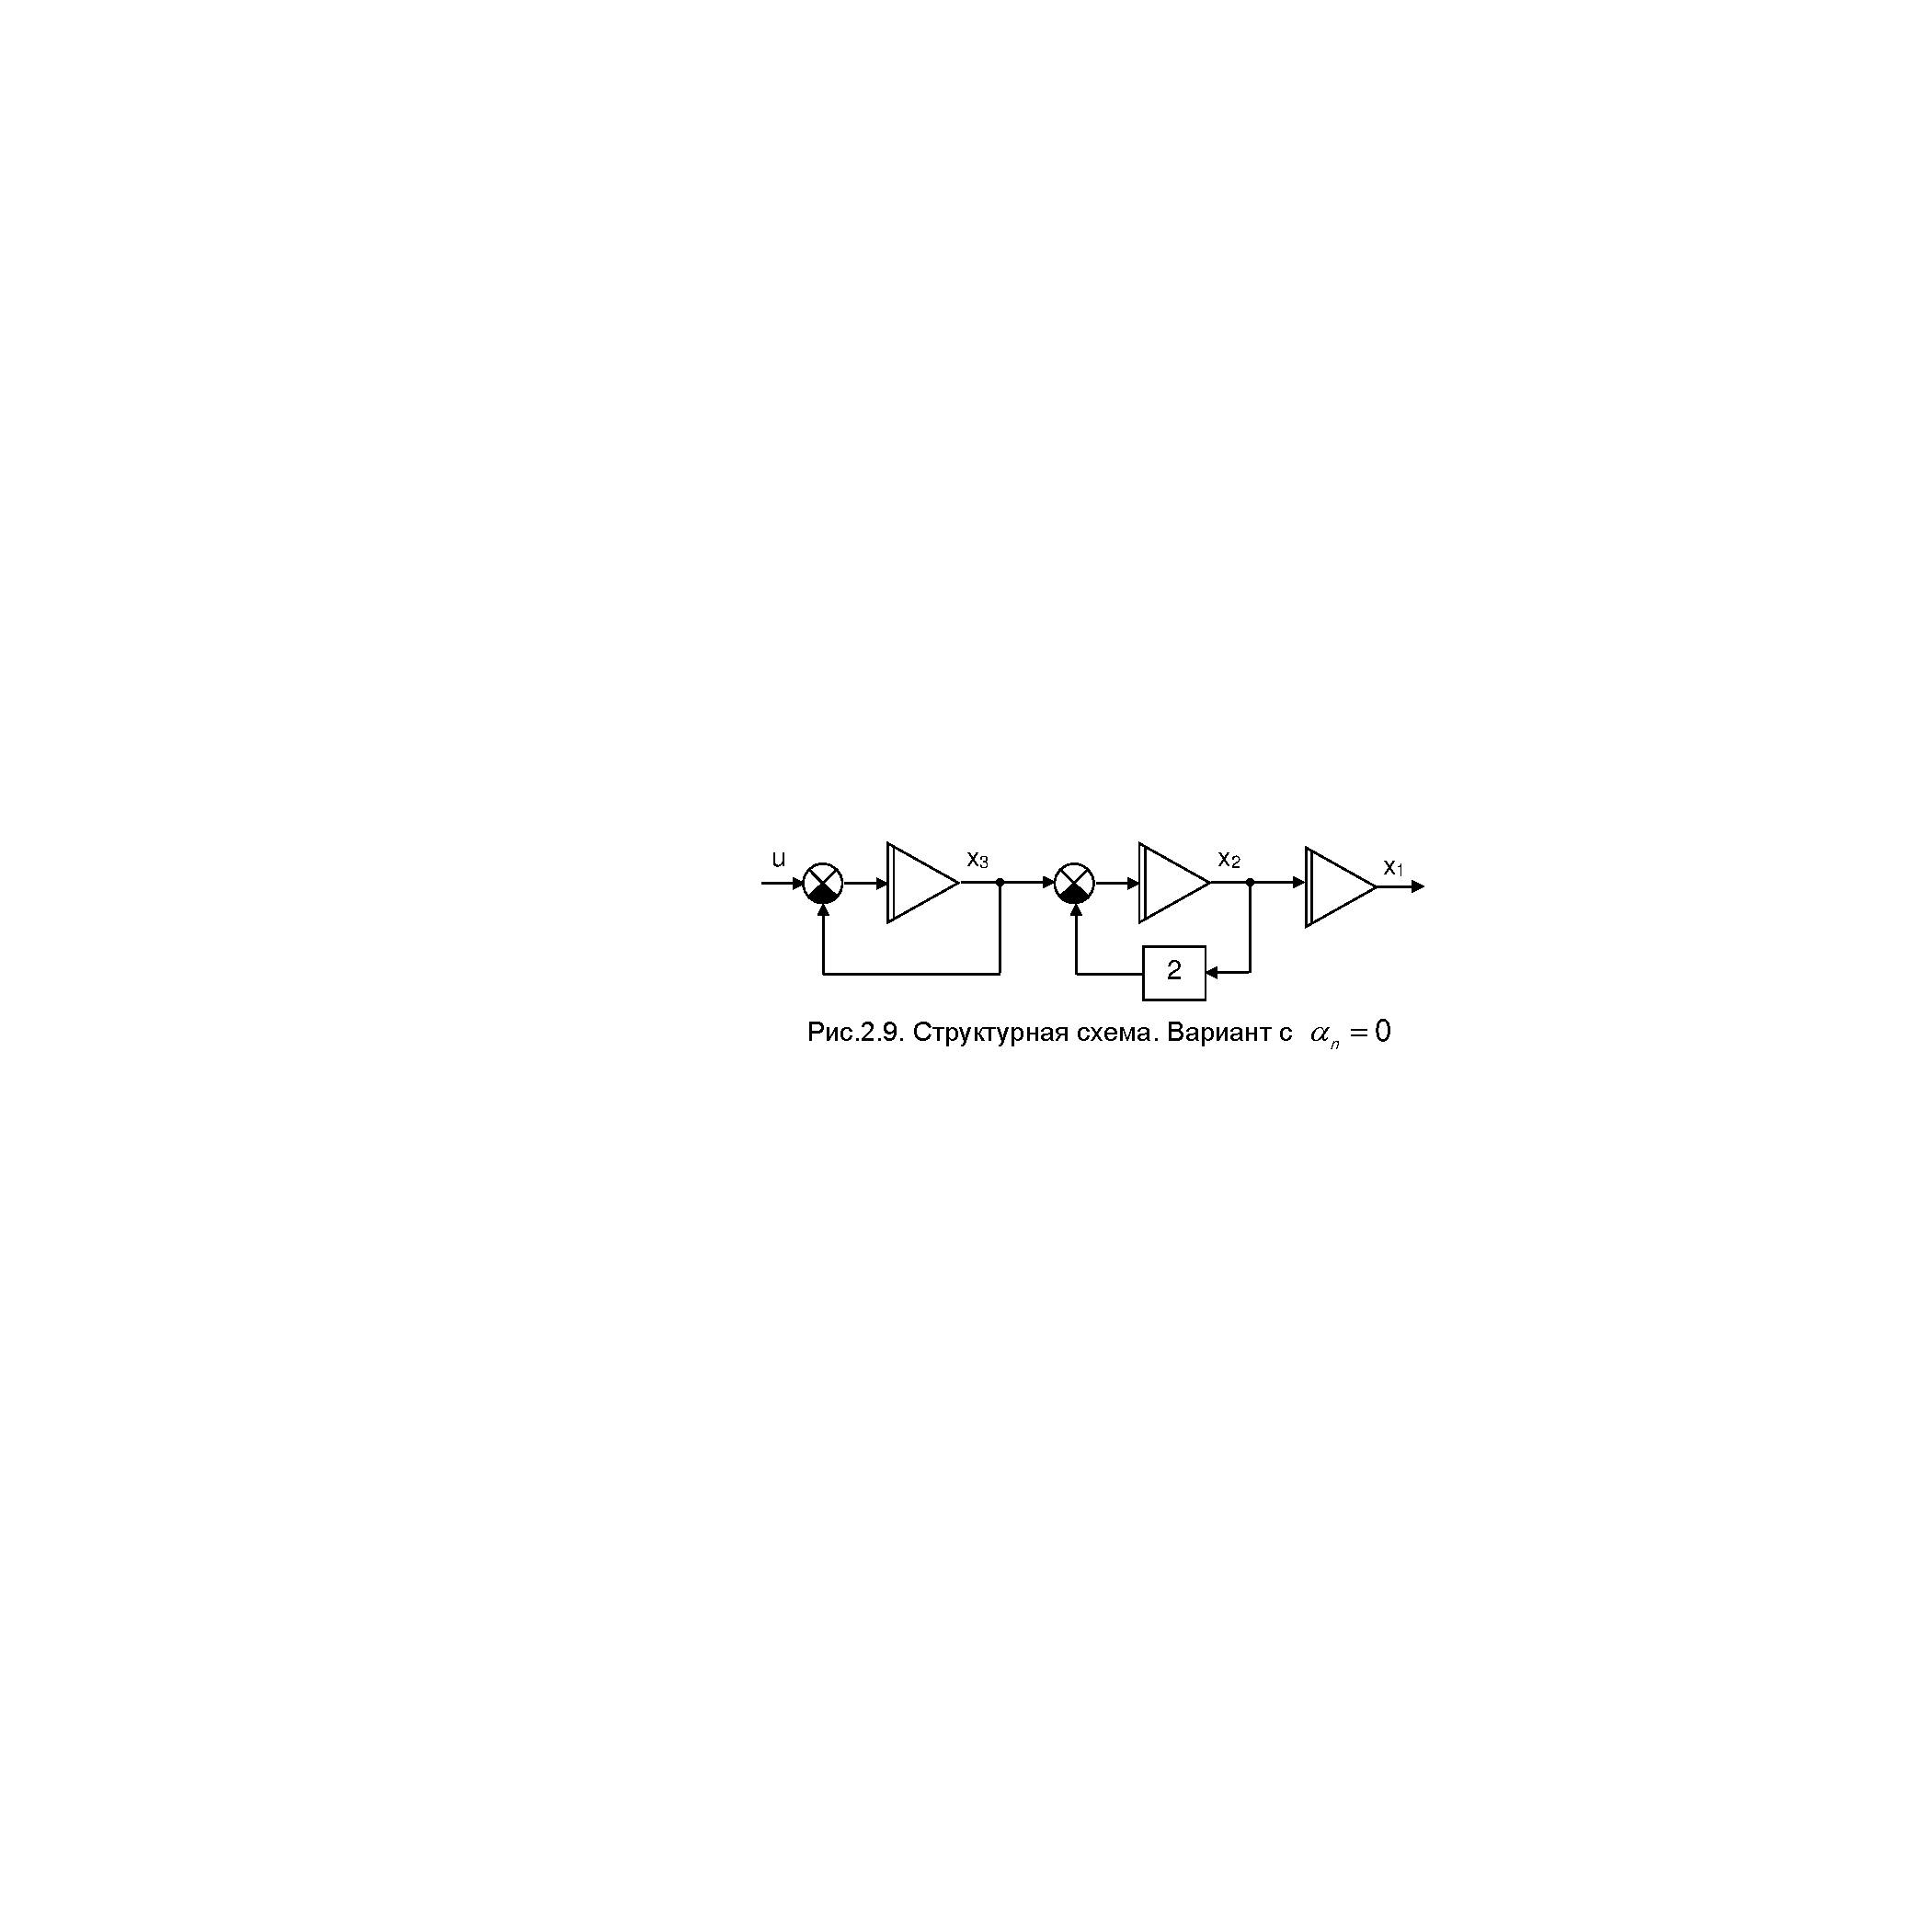
\includegraphics[width=12.356cm,height=4.339cm]{img-018}
	\caption{Структурная схема. Вариант с $ \alpha_{n}=0 $}
\end{figure}


\bigskip

\subsection{Собственные значения и собственные векторы   транспонированной матрицы}
		Собственные значения транспонированной матрицы - это такие  $\lambda $, для которых система уравнений



	\begin{equation}\label{key}
		 A^T\vec d=\lambda \vec d  (2.4.7)
	\end{equation}



		имеет нетривиальные решения, т.е. когда



\begin{equation}\label{key}
		  |\mathit{\lambda E}-A^T|=0.  (2.4.8)
\end{equation}



		Решение этого алгебраического уравнения дает  $n$ значений собственных чисел  $\lambda _1\;,\;\;\lambda _2\;,\;\;...\;,\;\;\lambda _n$. Так
		как определители квадратной матрицы и её транспонированной матрицы равны, то собственные числа матриц  $A$ и  $A^T$
		также равны. 



		Таким образом, собственному числу  $\lambda _i$ соответствует собственный вектор  $\vec v_i$ матрицы  $A$ и \ собственный
		вектор  $\vec d_i$ матрицы  $A^T$.



		Если транспонировать обе части уравнения \ (2.4.7), то получим



		   \begin{equation}\label{key}
		    \vec d^TA=\lambda \vec d^T.  
		    (2.4.9)
		   \end{equation}



		В связи с этим вектор  $\vec d$ называют левым собственным вектором матрицы  $A$, в отличие от  $\vec v$, который, в
		таком случае, называют правым собственным вектором. Для  $i$-го собственного числа и  $i$-го левого собственного
		вектора соответственно



		\begin{equation*}\label{key}
		\vec d_i^TA=\lambda _i\vec d_i^T.
		\end{equation*}



		Умножим обе части этого равенства справа на вектор  $\vec v_j$:



		\begin{equation}\label{key}
		\vec d_i^TA\vec v_j=\lambda _i\vec d_i^T\vec v_j.  (2.4.10)
		\end{equation}



		Учитывая свойства собственных векторов, в результате получаем уравнение



	\begin{equation*}\label{key}
	\vec d_i^T\lambda _j\vec v_j=\lambda _i\vec d_i^T\vec v_j,
	\end{equation*}



		которое \ преобразуется к виду



		\begin{equation}\label{key}
		  \vec d_i^T\vec v_j(\lambda _j-\lambda _i)=0.  (2.4.11)
		\end{equation}



		Полагаем, что все собственные числа матрицы  $A$ различны. Тогда для %TODO$  $
	имеем  $\lambda _i\neq \lambda _j$ и из равенства (2.4.11) следует, что
		векторы  $\vec d_i^T$ и  $\vec v_j$ взаимно ортогональны:


\begin{equation}\label{key}
		  \vec d_i^T\vec v_j=0\;,\;\;\;\;i\neq j.  (2.4.12)
\end{equation}



		Это означает то, что  $\vec d_i$ ортогонален  $(n-1)$\textit{ }- мерной гиперплоскости с базисом, образованным векторами
		$\vec v_j$ для всех  $j\neq i$.



		В качестве примера \ на рис. 2.10 показан один из вариантов взаимного расположения правых и левых собственных векторов
		некоторой матрицы  $A$ для случая  $n=3$. Здесь хорошо видно, что каждый \ из векторов  $\vec d_i$ ортогонален всем
		векторам  $\vec v_i$ при  $j\neq i$.

\begin{figure}[h]
	\centering  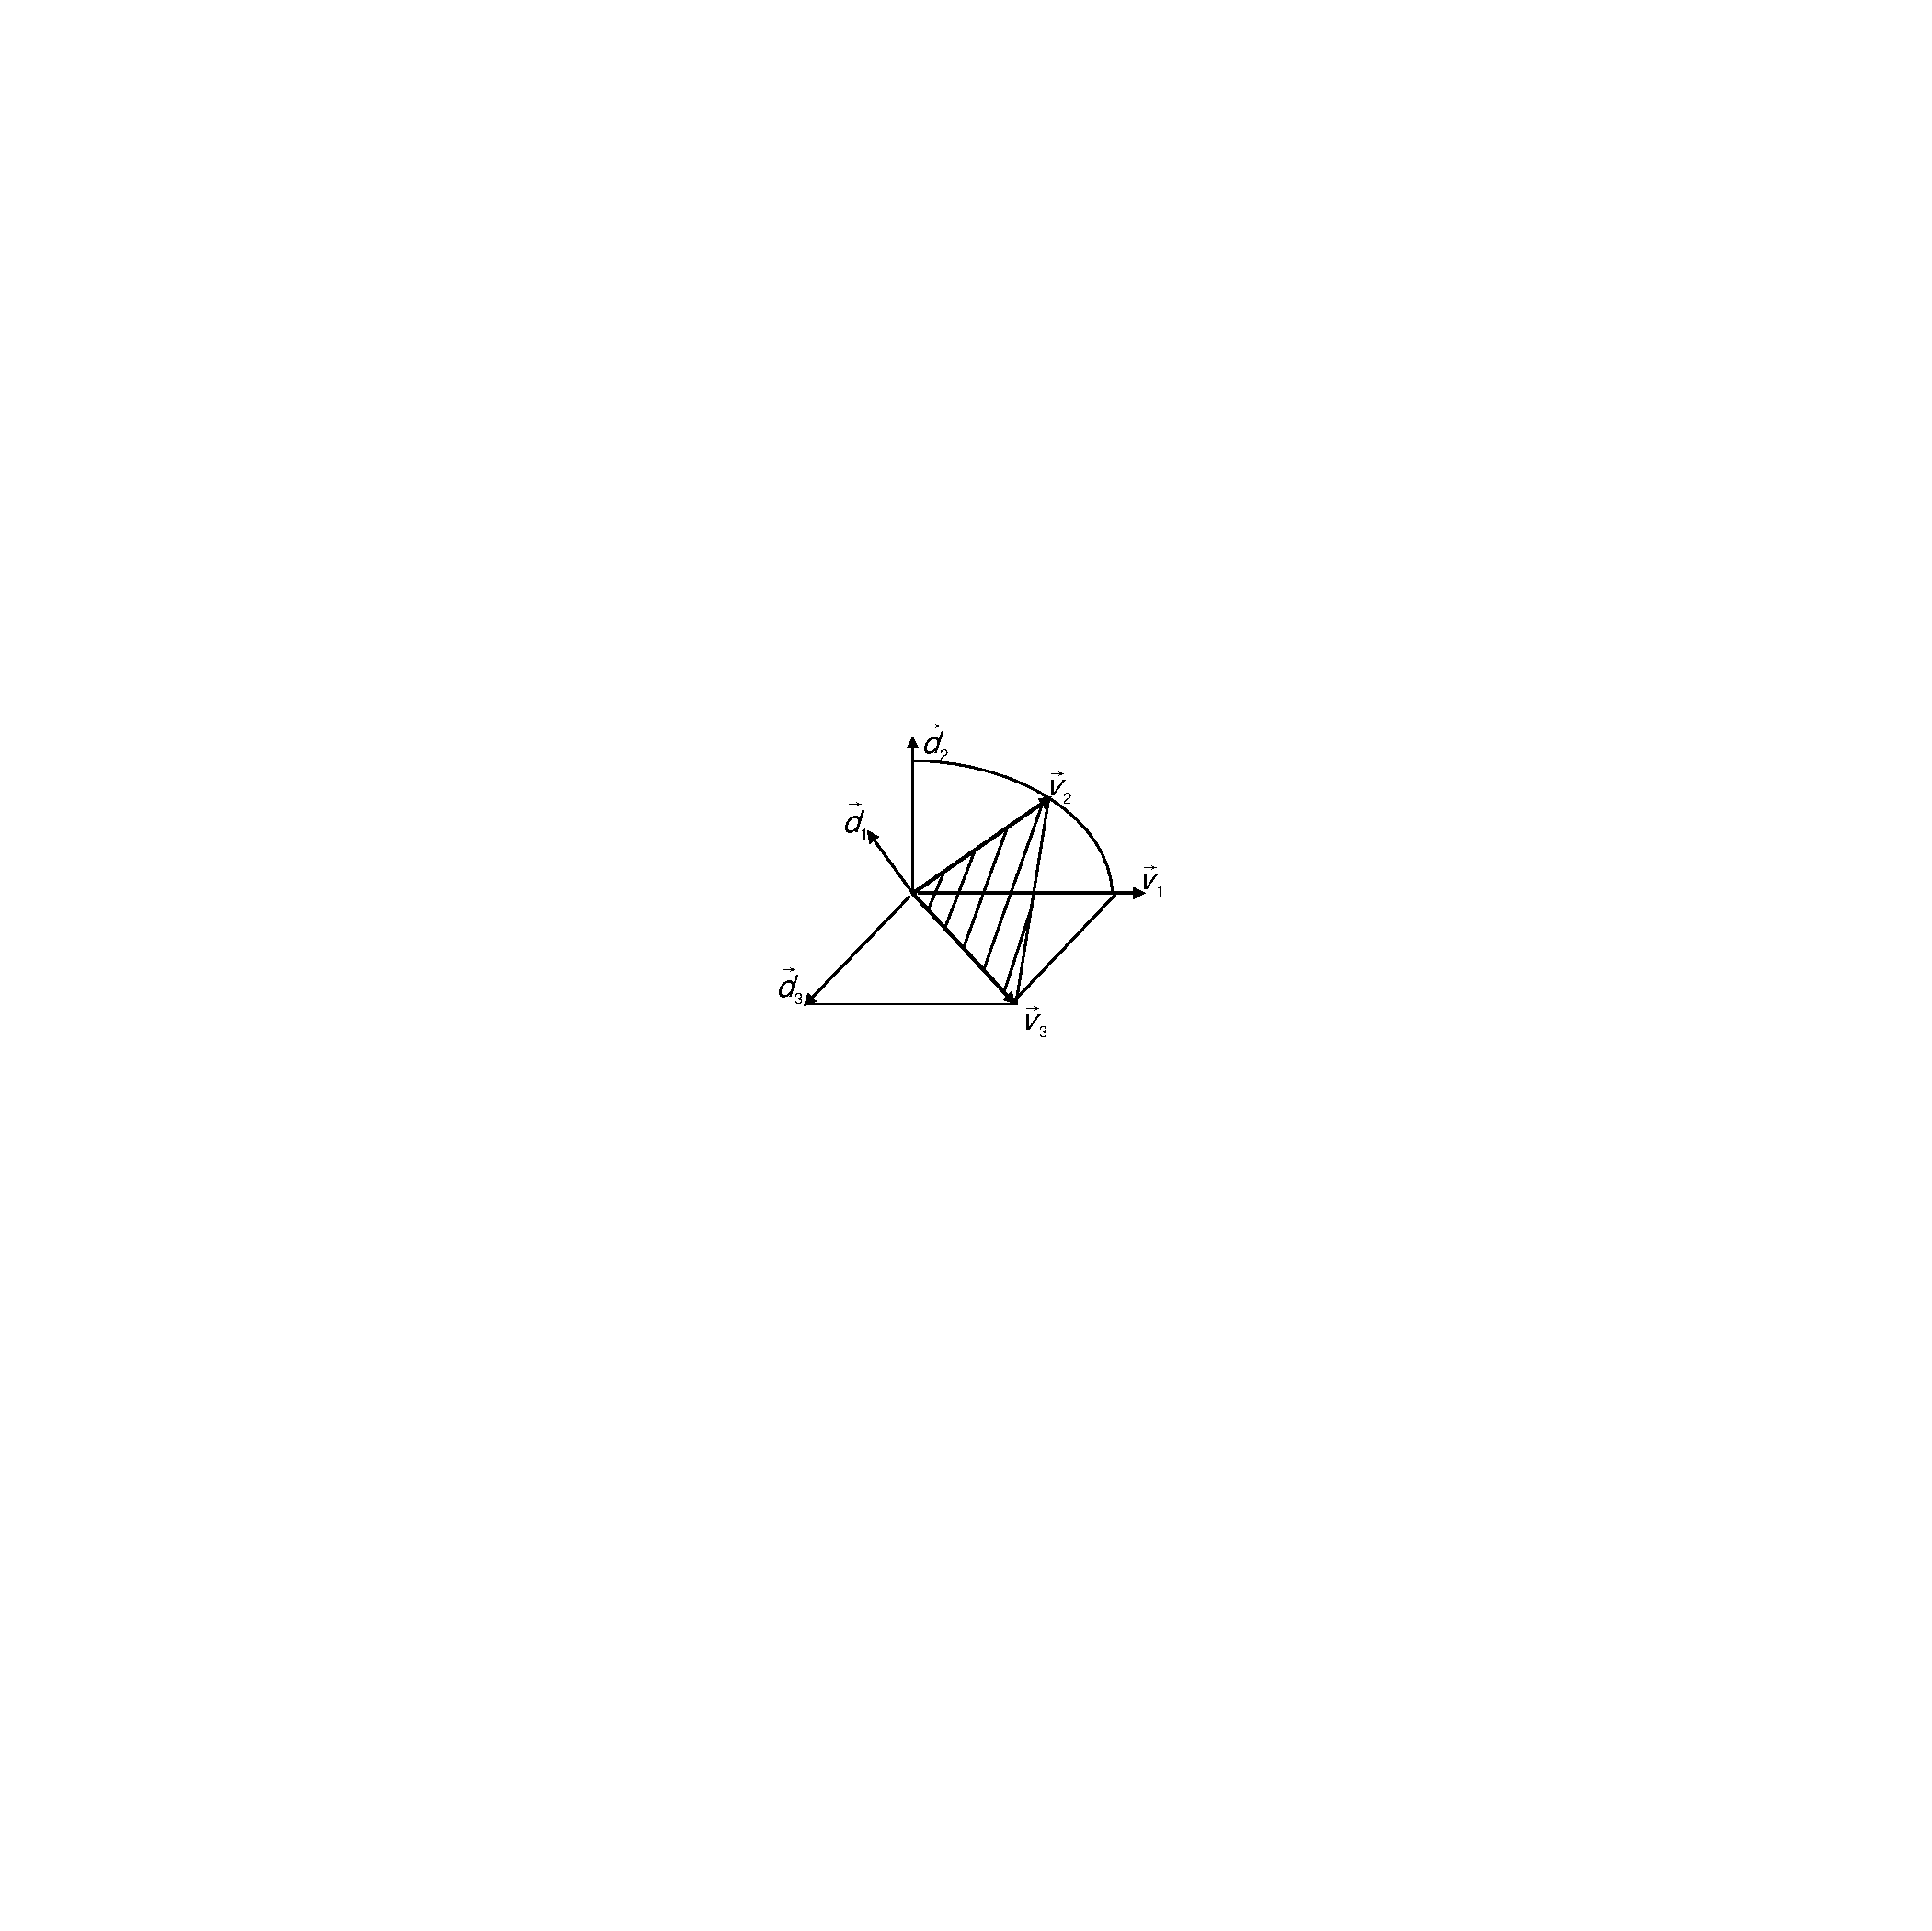
\includegraphics[scale=0.99]{img-020}
	\caption{Пример взаимного расположения правых и левых собственных векторов}
\end{figure}

\bigskip


		Теперь рассмотрим случай, когда  $i=j$. При этом скалярные произведения векторов  $\vec d_i$ и  $\vec v_i$ не должны
		быть равны нулю. Если предположить, что  $\vec d_i^T\vec v_i=0$, \ то придется утверждать, что вектор  $\vec d_i$
		ортогонален всему \textit{n} – мерному пространству с базисом  $\vec v_1,\;\vec v_2,\;\;\ldots \;\;,\;\vec v_n$. Но
		этого не может быть, так как вектор  $\vec d_i$ сам принадлежит этому пространству. Таким образом,


%TODO понять что тут не так 
%\begin{equation}\label{key}
%		\vec d_i^T\vec v_i\neq 0\;\;\;\;$ для \  $i=1\;,\;\;2\;,\;\;...\;,\;\;n.\ \ (2.4.13)
%\end{equation}



		В связи с тем, что собственные векторы можно выбирать с точностью до постоянного (в том числе комплексного) сомножителя,
		то наборы, иначе говоря, базисы  $\left\{\vec v\right\}$ и  $\left\{\vec d\right\}$ формируют так, чтобы для 
		$i=1\;,\;\;2\;,\;\;...\;,\;\;n$ выполнялось условие



		\ \  $\vec d_i^T\vec v_i=1\;\;\;\;\text{для}\;\;\;i=1\;,\;\;2\;,\;\;...\;,\;\;n$.\ \ (2.4.14)



		Отметим ещё одно важное свойство собственных векторов:



		\textit{Если матрица } $A$\textit{ не имеет кратных собственных чисел, то все её собственные векторы линейно независимы,
			то есть образуют базис в пространстве } $R^n$\textit{.} 



		Это нетрудно доказать. Действительно, предположим сначала, что среди собственных векторов матрицы  $A$ первые два
		являются линейно зависимыми, то есть



\begin{equation}\label{eq:vectormatrixA}
	\overset 2{\underset{i=1}{\sum }}\gamma_i\vec v_i=0,  (2.4.15)
\end{equation}



		где ни один из коэффициентов  $\gamma_1$ и  $\gamma_2$ не равен нулю. Умножив это уравнение слева на  $A$, получим



\begin{equation}\label{key}
	\overset 2{\underset{i=1}{\sum }}\gamma_i\lambda _i\vec v_i=0.  (2.4.16)
\end{equation}



		Теперь умножим \eqref{eq:vectormatrixA}(2.4.15) на  $\lambda _2$:



	\begin{equation}\label{key}
		\overset 2{\underset{i=1}{\sum }}\gamma_i\lambda _2\vec v_i=0.  (2.4.17)
	\end{equation}



		Вычтем (2.4.17) из (2.4.16) и в результате получим



\begin{equation*}\label{key}
		\ \  \gamma_1(\lambda _1-\lambda _2)\vec v_1=0.
\end{equation*}



		Из того, что  $\lambda _1\neq \lambda _2$ и  $\gamma_1\neq 0$, следует  $\vec v_1=0$, чего не может быть, следовательно, первые два
		собственных вектора не могут быть линейно зависимыми.



		\ \ Теперь предположим, что число линейно зависимых векторов равно  $r>2$, то есть



\begin{equation*}\label{key}
		\ \  \overset r{\underset{i=1}{\sum }}\gamma_i\vec v_i=0,\ \gamma_i\neq 0;\ i=1,2,\;\ldots \;,\;r.\ \ 
\end{equation*}



		Умножив это уравнение слева на  $A$, получим



		\ \  $\overset r{\underset{i=1}{\sum }}\gamma_i\lambda _i\vec v_i=0$.  (2.4.18)



		Умножим (2.4.18) на  $\lambda _r$:



		\ \  $\overset r{\underset{i=1}{\sum }}\gamma_i\lambda _r\vec v_i=0$.  (2.4.19)



		Вычтем (2.4.19) из (2.4.18) и в результате будем иметь

$ \gamma $

		\ \  $\overset{r-1}{\underset{i=1}{\sum }}\gamma_i(\lambda _i-\lambda _r)\vec v_i=0$.



		Получается, что число линейно зависимых векторов  $r-1<r$. Если согласиться с этим, то дойдём до  $r=2$, и круг
		замкнулся.



		Таким образом, действительно, все собственные векторы матрицы  $A$ являются линейно независимыми, поэтому \ матрица 
		$V=\left[\vec v_1\;,\;\;\vec v_2\;,\;\;...\;,\;\;\vec v_n\right]$, построенная из векторов базиса  $\left\{\vec
		v\right\}$, т.е. из правых собственных векторов матрицы $A$, является невырожденной. Эта матрица называется модальной
		матрицей. Из перечисленных выше свойств для правых и левых собственных векторов следует равенство



		\begin{equation}\label{key}
			D^TV=E, или  D^T=V^{-1}, (2.4.20)
		\end{equation}



		где  $D^T$- матрица, строки которой являются транспонированными векторами двойственного базиса  $\left\{\vec d\right\}$,
		т.е. левыми собственными векторами матрицы  $A$:



\begin{equation}\label{key}
	D^T=\left[
	\begin{matrix}
	\vec d_1^T\\\vec d_2^T\\\cdot \cdot \cdot \\\vec
	d_n^T
	\end{matrix}
	\right].  (2.4.21)
\end{equation}



\bigskip

\subsection{Определение функции от матрицы через её левые и правые собственные векторы}

\bigskip


		Все n систем уравнений


\begin{equation*}
A\vec v_i=\lambda _i\vec v_i,_{}^{}i=1,2,...,n
\end{equation*}

		могут быть записаны с использованием блочных матриц:



\begin{equation*}
		[A\vec v_1^{}A\vec v_2^{}...^{}A\vec v_n]=[\lambda _1\vec v_1^{}\lambda _2\vec v_2^{}...^{}\lambda _n\vec v_n].
\end{equation*}



		Учтем, что
\begin{equation*}
[A\vec v_1^{}A\vec v_2^{}...^{}A\vec v_n]=\normalsubformula{\text{AV}}
\end{equation*}
		и
\begin{equation*}
\left[\begin{matrix}\lambda _1\vec v_1&\lambda _2\vec v_2&\cdots &\lambda _n\vec v_n\end{matrix}\right]=
\end{equation*}
\begin{equation*}
=\left[\begin{matrix}v_{11}&v_{12}&\cdots &v_{1n}\\v_{21}&v_{22}&\cdots &v_{2n}\\\cdots &\cdots &\cdots &\cdots
\\v_{\mathit{n1}}&v_{\mathit{n2}}&\cdots &v_{\normalsubformula{\text{nn}}}\end{matrix}\right]\cdot
\left[\begin{matrix}\lambda _1&0&\cdots &0\\0&\lambda _2&\cdots &0\\\cdots &\cdots &\cdots &\cdots \\0&0&\cdots
&\lambda _n\end{matrix}\right]=\mathit{V\Lambda }\;,
\end{equation*}

		где  $\Lambda $--- диагональная матрица собственных чисел.



		Таким образом, получено равенство



	\begin{equation*}
		 \text{AV}=\mathit{V\Lambda },
	\end{equation*}
	или
\begin{equation}\label{key}
	A=\mathit{V\Lambda D}^T.\ \ (2.4.22)
\end{equation}



		\textit{Преобразование } $A=\normalsubformula{\text{TCT}}^{-1}$\textit{, где } $T$\textit{ - произвольная невырожденная
			матрица, называется преобразованием подобия}. Одно из основных свойств этого преобразования заключается в том, что
		собственные числа подобных матриц (здесь -  $A$ и  $C$) совпадают. Действительно,



		
\begin{equation}\label{key}
		\varphi _A(\lambda )=|\mathit{\lambda E}-A|=|\lambda \normalsubformula{\text{TT}}^{-1}-\normalsubformula{\text{TCT}}^{-1}|=|T||\mathit{\lambda E}-C||T^{-1}|=\varphi _C(\lambda ).
\end{equation}



		Говорят, что матрица  $A$ приводится к диагональному виду преобразованием



\begin{equation}\label{key}
	\Lambda =V^{-1}\normalsubformula{\text{AV}}=D^T\normalsubformula{\text{AV}}.(2.4.23)
\end{equation}



		Более высокие степени  $A$ приводятся к диагональному виду таким же способом:


\begin{equation*}
\Lambda ^2=V^{-1}\normalsubformula{\text{AVV}}^{-1}\normalsubformula{\text{AV}}=V^{-1}A^2V
\end{equation*}
		  .....................................................
	%TODO что то не так
\begin{equation*}\label{key}
	\Lambda ^l=V^{-1}A^lV или  A^l=\mathit{V\Lambda }^lV^{-1}.s
\end{equation*}
		Таким образом, если рассмотреть матричный многочлен 
\begin{equation*}
N(A)=A^l+C_1A^{l-1}+\ldots +C_{l-1}A+C_lE,
\end{equation*}
		то 
\begin{equation*}
N(A)=V\left\{\Lambda ^l+C_1\Lambda ^{l-1}+\ldots +C_{l-1}\Lambda +C_lE\right\}V^{-1},
\end{equation*}
		или
\begin{equation}\label{key}
		  N(A)=V\left[
		\begin{matrix}
		N(\lambda _1)&0&\cdot \cdot \cdot &0\\0&N(\lambda _2)&\cdot \cdot \cdot &0\\\cdot \cdot \cdot &\cdot
		\cdot \cdot &\cdot \cdot \cdot &\cdot \cdot \cdot \\0&0&\cdot \cdot \cdot
		&N(\lambda _l)
		\end{matrix}
		\right]V^{-1}.
		(2.4.24)
\end{equation}


		Если применить этот результат к характеристическому полиному, то получим
\begin{equation}\label{key}
 		\varphi (A)=0,  
 		(2.4.25) 
\end{equation}
		то есть \textit{каждая квадратная матрица удовлетворяет своему харак­те­ри­сти­ческому полиному}. Это утверждение
		известно в теории матриц как \textit{теорема Кэли-Гамильтона}.



		Для любой функции от матрицы  $f(A)$, которую можно представить в виде конечного или бесконечного степенного полинома,
		справедливо аналогичное выражение



\begin{equation}\label{key}
	f(A)=V\cdot \left[\begin{matrix}f(\lambda_{1})&0&\ldots &0\\0&f(\lambda_{2})&\ldots &0\\\vdots &\vdots &&\vdots \\0&0&\ldots
		&f(\lambda_{n})\end{matrix}\right]\cdot D^{T}(2.4.26)
\end{equation}



		или эквивалентное ему



		   $f(A)=\overset n{\underset{i=1}{\sum }}f(\lambda _i)\vec v_i\vec d_i^T.$\ \ (2.4.27)



		Отсюда вытекает, например, один из способов определения матричной экспоненты или соответствующей переходной матрицы:



		\ \  $\Phi (t)=e^{\normalsubformula{\text{At}}}=\overset n{\underset{i=1}{\sum }}e^{\lambda _it}\vec v_i\vec d_i^T.$\ \ (2.4.28)



\bigskip


		ПРИМЕР 2.4.2. Для объекта, представленного на рис.2.8 в примере 2.4.1, найдём левые собственные векторы. Если обозначить
		присоединённую матрицу к матрице  $A$ как  $I\{A\}$, то очевидно равенство 



		\ \  $I\{A^T\}=I^T\{A\}$.



		Поэтому



		$I^d(\lambda )=I\{A^T\}=\left[\begin{matrix}\lambda ^2+3\lambda +2&0&0\\\lambda +1&\lambda ^2+4\lambda +3&0\\1&\lambda +3&\lambda ^2+5\lambda +6\end{matrix}\right]$.



		Учитывая, что



		\ \  $\lambda _1=-1;\;\;\;\lambda _2=-2;\;\;\;\lambda _3=-3$,



		имеем


\begin{equation*}
I^d(\lambda _1)=\left[\begin{matrix}0&0&0\\0&0&0\\1&2&2\end{matrix}\right]\;;\;\;\;\;\;I^d(\lambda _2)=\left[\begin{matrix}0&0&0\\-1&-1&0\\1&1&0\end{matrix}\right];
\end{equation*}
\begin{equation*}
I^d(\lambda _3)=\left[\begin{matrix}2&0&0\\-2&0&0\\1&0&0\end{matrix}\right]\;.
\end{equation*}

		Рассчитаем левые собственные векторы. Учтем при этом (2.4.14). Таким образом, для первого собственного вектора  $\vec
		d_1$ должны выполняться условия

%$ \upsilon \varupsilon$
%		\ \  $\vec d_1^T=vν_1\left[\begin{matrix}0&0&1\end{matrix}\right]\;,\;\;\;\;\;\vec d_1^T\vec v_1=2ν_1=1$,



		откуда 



%		\ \  $ν_1=\frac 1 2$ \ \ \ и \ \ \  
%		$\vec d_1^T=\left[\begin{matrix}0&0&0.5\end{matrix}\right]$.



		Аналогично получим



		\ \  $\vec d_2=\left[\begin{matrix}0\\1\\-1\end{matrix}\right];_{}^{}\vec
		d_3=\left[\begin{matrix}1\\-1\\0.5\end{matrix}\right]$.



		Теперь можно записать выражение для переходной матрицы. Из (2.4.28) имеем


\begin{equation*}
e^{\normalsubformula{\text{At}}}=\left[\begin{matrix}0&0&0.5\\0&0&1\\0&0&1\end{matrix}\right]e^{-t}+\left[\begin{matrix}0&1&-1\\0&1&-1\\0&0&0\end{matrix}\right]e^{-2t}+\left[\begin{matrix}1&-1&0.5\\0&0&0\\0&0&0\end{matrix}\right]e^{-3t}
\end{equation*}

		и окончательно



		\ \ 
		$e^{\normalsubformula{\text{At}}}=\left[\begin{matrix}e^{-3t}&e^{-2t}-e^{-3t}&0.5e^{-t}-e^{-2t}+0.5e^{-3t}\\0&e^{-2t}&e^{-t}-e^{-2t}\\0&0&e^{-t}\end{matrix}\right]$.



		Рассмотрим ещё несколько примеров.



		Для


\begin{equation*}
A=\left[\begin{matrix}-3&1&0\\0&-2&1\\0&0&-1\end{matrix}\right]\;;\;\;\;\;\;\;\;\;\;\lambda _1=-1\;;\;\;\;\lambda _2=-2\;;\;\;\;\;\lambda _3=-3
\end{equation*}

		имеем


\begin{equation*}
\begin{matrix}\sqrt A=j\left[\begin{matrix}0\hfill\null &0\hfill\null &\frac 1 2\hfill\null \\0\hfill\null &0\hfill\null
&1\hfill\null \\0\hfill\null &0\hfill\null &1\hfill\null \end{matrix}\right]+j\sqrt 2\left[\begin{matrix}0\hfill\null
&1\hfill\null &-1\hfill\null \\0\hfill\null &1\hfill\null &-1\hfill\null \\0\hfill\null &0\hfill\null &0\hfill\null
\end{matrix}\right]+j\sqrt 3\left[\begin{matrix}1\hfill\null &-1\hfill\null &0.5\hfill\null \\0\hfill\null
&0\hfill\null &0\hfill\null \\0\hfill\null &0\hfill\null &0\hfill\null \end{matrix}\right]=\hfill\null
\\=j\left[\begin{matrix}\sqrt 3\hfill\null &\sqrt 2-\sqrt 3\hfill\null &\frac 1 2-\sqrt 2+\frac{\sqrt 3} 2\hfill\null
\\0\hfill\null &\sqrt 2\hfill\null &1-\sqrt 2\hfill\null \\0\hfill\null &0\hfill\null &1\hfill\null
\end{matrix}\right].\hfill\null \end{matrix}\hfill 
\end{equation*}

		Проведём проверку:


\begin{equation*}
\begin{matrix}j^2\left[\begin{matrix}\sqrt 3\hfill\null &\sqrt 2-\sqrt 3\hfill\null &\frac 1 2-\sqrt 2+\frac{\sqrt 3}
2\hfill\null \\0\hfill\null &\sqrt 2\hfill\null &1-\sqrt 2\hfill\null \\0\hfill\null &0\hfill\null &1\hfill\null
\end{matrix}\right]\cdot \left[\begin{matrix}\sqrt 3\hfill\null &\sqrt 2-\sqrt 3\hfill\null &\frac 1 2-\sqrt
2+\frac{\sqrt 3} 2\hfill\null \\0\hfill\null &\sqrt 2\hfill\null &1-\sqrt 2\hfill\null \\0\hfill\null &0\hfill\null
&1\hfill\null \end{matrix}\right]=\hfill\null \\=\left[\begin{matrix}-3\hfill\null &1\hfill\null &0\hfill\null
\\0\hfill\null &-2\hfill\null &1\hfill\null \\0\hfill\null &0\hfill\null &-1\hfill\null \end{matrix}\right].\hfill\null
\end{matrix}\hfill 
\end{equation*}

\bigskip


		Для той же матрицы найдём  $A^5$:



		$\lambda _1^5=-1\;,\;\;\;\;\;\lambda _2^5=-32\;,\;\;\;\;\;\lambda _3^5=-243$ \ \ \ и


\begin{equation*}
\begin{matrix}A^5=-\left[\begin{matrix}0\hfill\null &0\hfill\null &\frac 1 2\hfill\null \\0\hfill\null &0\hfill\null
&1\hfill\null \\0\hfill\null &0\hfill\null &1\hfill\null \end{matrix}\right]-32\left[\begin{matrix}0\hfill\null
&1\hfill\null &-1\hfill\null \\0\hfill\null &1\hfill\null &-1\hfill\null \\0\hfill\null &0\hfill\null &0\hfill\null
\end{matrix}\right]-243\left[\begin{matrix}1\hfill\null &-1\hfill\null &\frac 1 2\hfill\null \\0\hfill\null
&0\hfill\null &0\hfill\null \\0\hfill\null &0\hfill\null &0\hfill\null \end{matrix}\right]=\hfill\null
\\=\left[\begin{matrix}-243\hfill\null &211\hfill\null &-90\hfill\null \\0\hfill\null &-32\hfill\null &31\hfill\null
\\0\hfill\null &0\hfill\null &-1\hfill\null \end{matrix}\right].\hfill\null \end{matrix}\hfill 
\end{equation*}
	
	\newpage
	\chapter{Синтез линейных непрерывных систем}
\setcounter{section}{8} %TODO:Remove
\setcounter{subsection}{2} %TODO:Remove
\setcounter{equation}{23} %TODO:Remove
\setcounter{figure}{7}%TODO:Remove

\subsection{Идентификационное каноническое представление системы с одним (скалярным) выходом}
С помощью рассуждений, аналогичных проведённым в п.3.8.1, можно получить следующие результаты.

Если пара матриц    полностью наблюдаема,  то  в   пространстве состояний  Х  всегда существует базис, в котором пара ${A,C}$  имеет идентификационное каноническое представление (ИКП):
\begin{equation}
	A_I = 
	\begin{bmatrix}
	    0 & 0 & \dots & 0 & 0 & -\alpha_n \\
	    1 & 0 & \dots & 0 & 0 & -\alpha_{n-1} \\
	    0 & 1 & \dots & 0 & 0 & -\alpha_{n-2} \\
	    \dots & \dots & \dots & \dots & \dots & \dots \\
	    0 & 0 & \dots & 0 & 0 & -\alpha_3 \\
	    0 & 0 & \dots & 1 & 0 & -\alpha_2 \\
	    0 & 0 & \dots & 0 & 1 & -\alpha_1
	\end{bmatrix}
\end{equation}

\begin{equation}
	C_I = 
	\begin{bmatrix}
	    0 & 0 & \dots & 0 & 0 & 1
	\end{bmatrix}
\end{equation}

Отметим, что

\begin{equation}
	A_I^T = A_U; C_I^T=\vec{b}_U.
\end{equation}

Если   в  некотором  исходном  базисе [$h$] заданы матрицы $A_H, C_H$ и если система полностью наблюдаема, то, для того чтобы вычислить их (матриц) ИКП, достаточно вычислить коэффициенты характеристичес¬кого полинома $\phi_A(\lambda)$ . После этого может быть вычислена матрица преобразования от исходного базиса [$h$] к ИКП в соответствии с (3.7.13):

\begin{equation}
	I_H^{-1}=N_I^{-1}N_H.
\end{equation}

Если известна матрица $B_H$ при векторе управления в исходном базисе, то с учётом (3.6.8)  в базисе ИКП она может быть определена с помощью соотношения

\begin{equation}
	B_I=I_H^{-1}B_H
\end{equation}

\subsection{Передаточная функция и структура для системы в ИКП}
В соответствии с видом матриц $A_I$ и $C_I$ уравнения системы со скалярным входом $u$ и скалярным выходом $y$  имеют вид

\begin{equation}
\begin{cases}
	\dot{x}_{i1} = -\alpha_nx_{in}+b_{i1}u;\\
	\dot{x}_{i2} = x_{i1} - \alpha_{n-1}x_{in}+b_{i2}u;\\
	\dot{x}_{i3} = x_{i2} - \alpha_{n-2}x_{in}+b_{i3}u;\\
	\begin{tabular}{ l l l l l l }
	  \dots & \dots & \dots & \dots & \dots & \dots 
	\end{tabular}
	\dot{x}_{in-1} = x_{in-2} - \alpha_{2}x_{in}+b_{in-1}u;\\
	\dot{x}_{in} = x_{in-1} - \alpha_{1}x_{in}+b_{in}u;\\
\end{cases}
\end{equation}

\begin{equation}
	y = x_{in}
\end{equation}

Этим уравнениям соответствует структурная схема, представленная на рис. 3.8.

\begin{figure}[H]
	\centering
	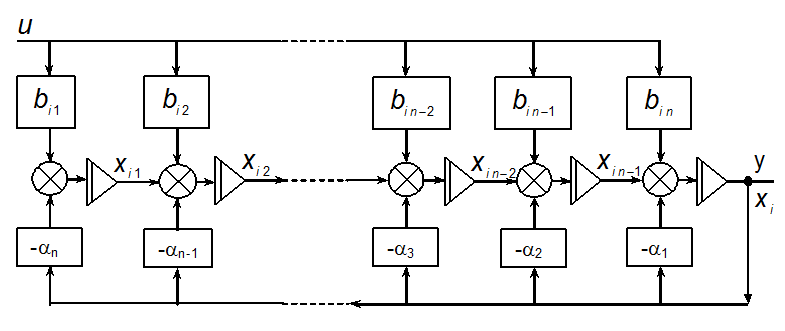
\includegraphics[scale=0.9]{images/Fig3_8}
	\caption{Схема моделирования системы в ИКП}
\end{figure}

В соответствии с этим рисунком передаточная функция системы имеет вид

\begin{multline}
	W_{u,y}(p) = \dfrac{b_{i1}p^{-n}+b_{i2}p^{-(n-1)}+\dots+b_{in-1}p^{-2}+b_{in}p^{-1}}{1+\alpha_1p^{-1}+\alpha_2p^{-2}+\dots+\alpha_np^{-n}} = \\
	\dfrac{b_{i1}+b_{i2}p+\dots+b_{in-1}p^{n-2}+b_{in}p^{n-1}}{p^n+\alpha_1p^{n-1}+\alpha_2p^{n-2}+\dots+\alpha_{n-1}p+\alpha_n}.
\end{multline}

Отметим, что статический передаточный коэффициент

\begin{equation}
	W_{u,y}(0)=\dfrac{b_{i1}}{\alpha_n}
\end{equation}

\newpage

\section{Обратная связь по состоянию, обеспечивающая заданное (желаемое) расположение собственных чисел в замкнутой системе с одним (скалярным) входом}

Даны уравнения полностью управляемого объекта управления в некотором исходном базисе

\begin{gather}
\begin{split}
	&\dot{\vec{x}}_H(t) = A_H\vec{x}_H(t)+\vec{b}_Hu(t);\\
	&y(t)=C_H\vec{x}_H(t),
\end{split}
\end{gather}
каждая координата вектора состояния которого доступна для измерения.
Требуется синтезировать такое управление, которое бы обеспечило требуемое качество отработки внешнего командного сигнала $v(t)$.

Динамические свойства системы управления в основном определяются её собственными числами, то есть нулями характеристического полинома
\begin{equation}
	\phi_A(\lambda) = \prod_{i=1}^{n}(\lambda - \lambda_i)=\lambda^n+\alpha_1\lambda^{n-1}+\dots+\alpha_n.
\end{equation}

Время переходного процесса каждой моды определяется расстоянием до мнимой оси вещественной части; колебательность - соотношением мнимой и вещественной частей соответствующих собственных чисел. Эти зависимости могут быть проанализированы при изучении характеристик типовых звеньев, кроме того, они рассматриваются в обширной учебной литературе по теории автоматического регулиро-вания и управления.

В соответствии со структурной схемой, приведённой на рис. 3.9, сформируем сигнал управления объектом в виде
\begin{equation}
	u(t) = L_H\vec{x}_H(t) + k^vv(t)
\end{equation}
где $L_H$ – некоторая матрица-строка обратной связи:
\begin{equation}
	L_H = [\begin{tabular}{ l l l l }
		  	$l_{h1}$ & $l_{h2}$ & $\dots$ & $l_{hn}$
		  \end{tabular}]
\end{equation}
$k^v$ – коэффициент по командному сигналу.
Тогда уравнение системы примет вид
\begin{equation}
	\dot{\vec{x}}_H(t)=A_H\vec{x}_H(t)+\vec{b}_HL_H\vec{x}_H(t)+\vec{b}_Hk^vv(t),
\end{equation}
или
\begin{equation}
	\dot{\vec{x}}_H(t)=A_H^C\vec{x}_H(t)+\vec{b}_Hk^vv(t),
\end{equation}
где $A_H^C$ - матрица замкнутой системы в исходном базисе:
\begin{equation}
	A_H^C=A_H+\vec{b}_HL_H
\end{equation}

\begin{figure}[H]
	\centering
	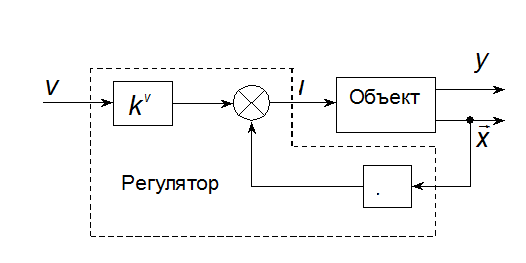
\includegraphics[scale=0.9]{images/Fig3_9}
	\caption{Структурная схема замкнутой системы}
\end{figure}

Поскольку объект полностью управляем, то существует базис [$u$], в котором пара $\{A,\vec{b}\}$ имеет управляемое каноническое представление $\{A_U,\vec{b}_U\}$ . Поэтому перейдём к записи уравнений системы в базисе УКП. В соответствии с (3.4.16) произведём замену 
\begin{equation}
	\vec{x}_H=U_H\vec{x}_U
\end{equation}
Тогда из (3.9.1) получим
\begin{equation}
	U_H\dot{\vec{x}}_U(t)=A_HU_H\vec{x}_U(t)+\vec{b}_Hu(t);
\end{equation}
\begin{equation}
	y(t)=C_HU_H\vec{x}_U.
\end{equation}
Умножив уравнение (3.9.9) слева на $U_H^{-1}$, будем иметь
\begin{gather}
\begin{split}
	&\dot{\vec{x}}_U(t)=A_U\vec{x}_U(t)+\vec{b}_Uu(t);\\
	&y(t) = C_U\vec{x}_U(t),
\end{split}
\end{gather}
где $A_U$ $\vec{b}_U$ и $C_U$ - соответствующие матрицы в УКП.

Используя подстановку (3.9.8), из (3.9.3) получим
\begin{equation}
	u(t)=L_U\vec{x}_U+k^vv(t),
\end{equation}
где матрица обратной связи в базисе УКП
\begin{equation}
	L_U=L_HU_H.
\end{equation}

В результате  уравнение замкнутой системы  в базисе управляемого канонического представле¬ния будет иметь вид
\begin{equation}
	\dot{\vec{x}}_U(t)=A_U^C\vec{x}_U(t)+\vec{b}_U \cdot k^vv(t)
\end{equation}
Здесь $A_U^C$ является сопровождающей матрицей по отношению к характеристическому полиному замкнутой системы
\begin{equation}
	\phi_{A^C}(\lambda) - \prod_{i=1}^{n}(\lambda - \lambda_i^3)=\lambda^n+\gamma_1\lambda^{n-1}+\dots+\gamma_n,
\end{equation}
поэтому она имеет стандартный вид
\begin{equation}
	A_U^C = 
	\begin{bmatrix}
	    0 & 1 & 0 & \dots & 0 \\
	    0 & 0 & 1 & \dots & 0 \\
	    \dots & \dots & \dots & \dots & \dots \\
	    0 & 0 & 0 & \dots & 1 \\
	    -\gamma_n &  -\gamma_{n-1} & -\gamma_{n-2} & \dots & -\gamma_1 \\
	\end{bmatrix}
\end{equation}
С другой стороны, очевидно, что
\begin{equation}
	A_U^C=A_U+\vec{b}_UL_U.
\end{equation}
Отсюда сразу же следует связь между коэффициентами характеристического полинома (3.9.2) объекта и коэффициентами характеристического полинома (3.9.14) желаемой системы:
\begin{equation}
	-\gamma_i=-\alpha_i+l_{Un-i+1}, i=1,2,\dots,n.
\end{equation}
Далее обусловлены следующие действия.
\begin{enumerate}
\renewcommand\labelenumi{\theenumi.}
\item Задание желаемых собственных чисел замкнутой системы $\lambda_1^3,\lambda_2^3,\dots,\lambda_n^3,$
\item Вычисление коэффициентов характеристического полинома замкнутой системы $\gamma_1,\gamma_2,\dots,\gamma_n$ в соответствии с выражением (3.9.15).
\item 3.	Вычисление согласно (3.9.17) коэффициентов матрицы обратной связи в базисе УКП:
\begin{equation}
	l_{U,n-i+1}=\alpha_i-\gamma_i, i=1,2,\dots,n.
\end{equation}
\item Вычисление в соответствии с (3.9.12) и (3.8.17) матрицы обратной связи в исходном базисе:
\begin{equation}
	L_H=L_UU_UU_H^{-1}.
\end{equation}
\item Определение величины коэффициента $k^v$ в соответствии с требованиями по статике.
\end{enumerate}

Так, например, если требуется обеспечить единичную статику по командному сигналу $v$, то это значит, что установившееся значение переходной функции $h(t)$ замкнутой системы должно быть равно единице. Одним из свойств передаточной функции устойчивой системы является равенство
\begin{equation}
	\lim\limits_{t\to\infty}h(t)=\lim\limits_{p\to0}W_{vy}(p)
\end{equation}
Согласно структурной схеме, приведённой на  рис. 3.9, передаточная функция между командным $v$ и выходным $y$ сигналами имеет вид
\begin{equation}
	W_{vy}(p)=k^v\cdot W(p)
\end{equation}
где передаточная функция $W(p)$ может быть определена аналогично выражению (3.8.22). Таким образом, получаем
\begin{equation}
	h(\infty)=k^v\dfrac{c_{U1}}{\gamma_n}=1,
\end{equation}
откуда, окончательно,
\begin{equation}
	k^v=\dfrac{\gamma_n}{c_U1}
\end{equation}
\newpage

\section{Синтез управления в многомерной системе. Задача разделения каналов}
В предыдущих разделах, посвящённых синтезу, рассматривались объекты со скалярным управлением (входом) и скалярным выходом. На практике встречаются и более сложные объекты. Один из них был упомянут в разделе 2.2. Это смесительный бак, у него две входные величины (два входных потока с различными концентрациями растворённого вещества) и две выходные (концентрация и расход выходного потока). В качестве другого примера может быть взят объект, связанный с перемоткой некоторой полосы с одного рулона на другой. Для этого объекта выходные переменные – это натяжение и линейная скорость перемотки; входные – напряжения или токи приводных двигателей моталки и разматывателя. Наконец, самолёт. В качестве выходных переменных могут выступать углы тангажа, курса и крена; в качестве входных, управляющих - угловые положения руля высоты, руля направления и элеронов.

Как правило, в таких объектах каждая выходная величина зависит от всех входных. В то же время при синтезе управления такими объектами часто требуется обеспечить не только заданные динамические и статические свойства системы, но и независимое управление по каждой из выходных переменных.

Пусть уравнения объекта имеют вид
\begin{equation}
	\dot{\vec{x}}(t)=A\vec{x}(t)+B\vec{u}(t);
\end{equation}
\begin{equation}
	\dot{\vec{y}}(t)=C\vec{x}(t),
\end{equation}
где размерность вектора состояния [$n\times1$] , вектор управления и век-тор выхода имеют одинаковую размерность [$p\times1$]. Такую же размер-ность имеет вектор командного сигнала $\vec{v}$, поступающий на вход системы. 

Требуется синтезировать управление $\vec{u}$ такое, чтобы:
\begin{enumerate}
\renewcommand\labelenumi{\theenumi)}
\item $i$–я составляющая вектора выхода $y_i$ зависела только от $i$–й составляющей командного сигнала $v_i$;
\item по каждому из каналов была обеспечена заданная динамика, иными словами, передаточная функция $W_{v_i,y_i}(p)=\dfrac{Y_i(p)}{V_i(p)}$, имеющая заданные полюсы;
\item для каждого из каналов был обеспечен заданный статический коэф-фициент передачи.
\end{enumerate}

\subsection{Разделение исходного объекта на подсистемы интеграторов}
Представим (3.10.2) в виде
\begin{equation*}
	\vec{y}=C\vec{x}= 
	\begin{bmatrix}
	    C_1  \\
	    C_2  \\
	    \vdots \\
	    C_p
	\end{bmatrix}
	\vec{x},
\end{equation*}
где $C_i$ - строки матрицы $C$. Тогда $i$-я координата вектора выхода
\begin{equation*}
	y_i=C_i\vec{x}
\end{equation*}

Рассмотрим процедуру многократного дифференцирования координат вектора выхода:
\begin{gather}
\begin{split}
	&y_i^{\prime}=C_i\dot{\vec{x}}=C_iA\vec{x}+C_iB\vec{u};\\
	&y_i^{\prime\prime}=C_iA^2\vec{x}+C_iAB\vec{u}+C_iB\vec{u}^{\prime};\\
	&y_i^{(3)}=C_iA^3\vec{x}+C_iA^2B\vec{u}+C_iAB\vec{u}^{(1)}+C_iB\vec{u}^{(2)};\\
	&\dots\dots\dots\dots\dots\dots\dots\dots\\
	&y_i^{(m)}=C_iA^m\vec{x}+C_iA^{m-1}B\vec{u}+C_iA^{m-2}B\vec{u}^{(1)}+\dots+C_iB\vec{u}^{(m-1)}.
\end{split}
\end{gather}
Сократим запись:
\begin{equation}
	y_i^{(m)}=C_iA^m\vec{x}+C_iA^{m-1}B\vec{u}+\sum_{v=1}^{m-1}C_iA^{m-1-v}B\vec{u}^{(v)}.
\end{equation}

Для каждой координаты найдем максимальное число дифференцирований, при котором еще не появляется производная вектора $\vec{u}$, то есть найдем такие числа $m_i$, что
\begin{equation*}
	C_iA^{m_i-1}B\neq0 \text{ и } C_iA^{m_i-2}B=0.
\end{equation*}
Таким образом, получим систему уравнений:
\begin{gather}
\begin{split}
	&y_1^{(m_1)}=C_1A^{m_1}\vec{x}+C_1A^{m_1-1}B\vec{u};\\
	&y_2^{(m_2)}=C_2A^{m_2}\vec{x}+C_2A^{m_2-1}B\vec{u};\\
	&\dots\dots\dots\dots\dots\dots\dots\dots\\
	&y_p^{(m_p)}=C_pA^{m_p}\vec{x}+C_pA^{m_p-1}B\vec{u};\\
\end{split}
\end{gather}
Запишем эту систему равенств в  векторно-матричном  виде:
\begin{equation}
	\begin{bmatrix}
	    y_1^{(m_1)}\\
	    y_2^{(m_2)}\\
	    \vdots \\
	    y_1^{(m_p)}\\
	\end{bmatrix}=
	\begin{bmatrix}
	    C_1A^{m_1}\\
	    C_2A^{m_2}\\
	    \vdots \\
	    C_1A^{m_p}\\
	\end{bmatrix}\vec{x}+
	\begin{bmatrix}
	    C_1A^{m_1-1}\\
	    C_2A^{m_2-1}\\
	    \vdots \\
	    C_1A^{m_p-1}\\
	\end{bmatrix}B\vec{u}=-F_*\vec{x}+B_*\vec{u}.
\end{equation}
Обозначим
\begin{equation}
	\vec{q}=
	\begin{bmatrix}
	    y_1^{(m_1)}\\
	    y_2^{(m_2)}\\
	    \vdots \\
	    y_1^{(m_p)}\\
	\end{bmatrix}
\end{equation}
и
\begin{equation}
	F_*=-
	\begin{bmatrix}
	    C_1A^{m_1}\\
	    C_2A^{m_2}\\
	    \vdots \\
	    C_1A^{m_p}\\
	\end{bmatrix};
	B_*=
	\begin{bmatrix}
	    C_1A^{m_1-1}\\
	    C_2A^{m_2-1}\\
	    \vdots \\
	    C_1A^{m_p-1}\\
	\end{bmatrix}B;
\end{equation}
Тогда (3.10.6) можно переписать в виде
\begin{equation}
	\vec{q}=-F_*\vec{x}+B_*\vec{u}.
\end{equation}
Если задача разделения каналов имеет решение, то матрица $B_*$ не вырождена и
\begin{equation}
	\vec{u}=B_*^{-1}\vec{q}+B_*^{-1}F_*\vec{x}.
\end{equation}

На рис. 3.10 представлена промежуточная структурная схема, соответствующая уравнениям (3.10.1), (3.10.2) и (3.10.8).
\begin{figure}[H]
	\centering
	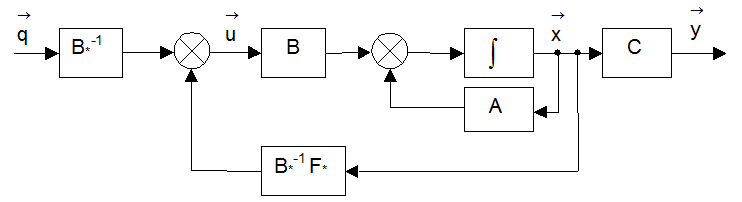
\includegraphics[scale=0.9]{images/Fig3_10}
	\caption{Промежуточная структурная схема}
\end{figure}
Для этой схемы справедливы уравнения
\begin{gather}
\begin{split}
	&\dot{\vec{x}}=(A+BB_*^{-1}F_*)\vec{x}+BB_*^{-1}\vec{q};\\
	&\vec{y}=C\vec{x}.
\end{split}
\end{gather}
Обозначим
\begin{gather}
\begin{split}
	&\underset{\lor}{A}=A+BB_*^{-1}F_*;\\
	&\underset{\lor}{B}=BB_*^{-1}.
\end{split}
\end{gather}
Теперь (3.10.11) превратится в 
\begin{equation}
\begin{cases}
	\dot{\vec{x}}=\underset{\lor}{A}\vec{x}+\underset{\lor}{B}\vec{q};\\
	\vec{y}=C\vec{x};
\end{cases}
\end{equation}
а структурная схема промежуточной системы с входным вектором $\vec{q}$ примет вид, представленный на рис. 3.11.
\begin{figure}[H]
	\centering
	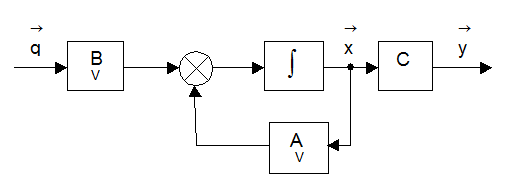
\includegraphics[scale=0.9]{images/Fig3_11}
	\caption{Структурная схема системы относительно входного вектора $\vec{q}$}
\end{figure}
С другой стороны, вектор выхода $\vec{y}$ связан с вектором $\vec{q}$ равенством (3.10.7), и поэтому схеме, представленной на рис. 3.11, полностью эквивалентна схема, составленная из $p$ подсистем последовательно включённых интеграторов. Эта схема представлена на рис. 3.12.
\begin{figure}[H]
	\centering
	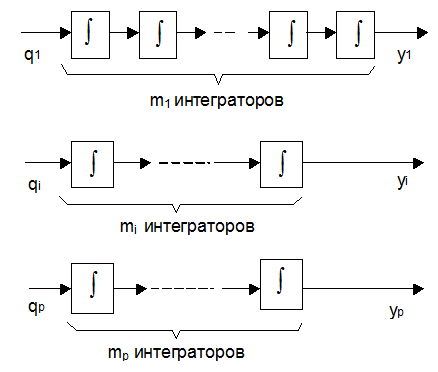
\includegraphics[scale=0.9]{images/Fig3_12}
	\caption{Структурная схема объекта, преставленного в виде изолированных подсистем интеграторов}
\end{figure}
Общее количество интеграторов не может быть больше $n$, то есть
\begin{equation*}
	\sum_{i=1}^{p}m_i\leq n.
\end{equation*}
Таким образом, система $\{\underset{\lor}{A},\underset{\lor}{B}\}$ (3.10.13), у которой в качестве входного вектора выбран вектор $\vec{q}$,

а) развязана по каналам, то есть $y_i$ зависит только от $q_i$ для всех значений $i$;

б) имеет $\sum_{i=1}^{p}m_i$ собственных значений, равных нулю.

Теперь систему $\{\underset{\lor}{A},\underset{\lor}{B}\}$ нужно попытаться привести к удобному базису, в котором следует синтезировать обратную связь, реализующую желаемые собственные числа по каждому каналу.

Прежде всего, установим некоторые свойства матриц $\underset{\lor}{A}$ и $\underset{\lor}{B}$. Аналогично (3.10.4) запишем:
\begin{equation*}
	y_i^{(m_i)}=C_i\underset{\lor}{A}^{m_i}\vec{x}+C_i\underset{\lor}{A}^{m_i-1}\underset{\lor}{B}\vec{q}+\sum_{v=1}^{m-1}C_i\underset{\lor}{A}^{m_i-1-v}\underset{\lor}{B}q^{(v)}.
\end{equation*}
С другой стороны, $y_i^{(m_i)}=q_i$. Отсюда следует:
\begin{equation}
	1) C_i\underset{\lor}{A}^{m_i}=0\text{ для всех }i=1,2,\dots,p;
\end{equation}
\begin{equation}
	2) C_i\underset{\lor}{A}^{m_i-1}\underset{\lor}{B}\vec{q}=C_i\underset{\lor}{A}^{m_i-1}
	\begin{bmatrix}
		 \underset{\lor}{\vec{b}_1} & \underset{\lor}{\vec{b}_2} & \dots & \underset{\lor}{\vec{b}_p}
	\end{bmatrix}\cdot
	\begin{bmatrix}
		 q_1\\q_1\\\vdots\\q_{ny}
	\end{bmatrix}=q_i,
\end{equation}
откуда
\begin{equation}
	C_i\underset{\lor}{A}^{m_i-1}\underset{\lor}{\vec{b}_i}=1;
\end{equation}
\begin{equation}
	C_i\underset{\lor}{A}^{m_i-1}\underset{\lor}{\vec{b}_j}=0,\text{ при } j\neq i;
\end{equation}
\begin{equation}
	3)C_i\underset{\lor}{A}^{m_i-v}\underset{\lor}{\vec{b}_j}=0,\text{ для } v>1 \text{ и для всех } j,i.
\end{equation}

\subsection{Преобразование базиса в пространстве $R^n$}
Перейдём от исходного базиса [$e$] к новому базису [$f$] с помощью некоторой матрицы преобразования $F_e$.  При выборе базиса [$f$] учтем следующие обстоятельства:
\begin{itemize}
\item объект управляем, поэтому ранг матрицы управляемости
\begin{equation}
	U=
	\setcounter{MaxMatrixCols}{20}
	\begin{bmatrix}
	\underset{\lor}{\vec{b}_1} & \underset{\lor}{\vec{b}_2} & \dots & \underset{\lor}{\vec{b}_p} & \vdots & \underset{\lor}{A}\underset{\lor}{\vec{b}_1} & \dots & \underset{\lor}{A}\underset{\lor}{\vec{b}_p} & \vdots & \dots & \vdots & \underset{\lor}{A^{n-1}}\underset{\lor}{\vec{b}_1} & \dots & \underset{\lor}{A^{n-1}}\underset{\lor}{\vec{b}_p}
	\end{bmatrix}
\end{equation} 
равен порядку системы;
\item так как каждый канал этой системы с размерностью $m_i$ управляем, то столбцы
\begin{equation*}
	\underset{\lor}{\vec{b}_1}, \underset{\lor}{A}\underset{\lor}{\vec{b}_1}, \dots, \underset{\lor}{A^{m_1-1}}\underset{\lor}{\vec{b}_1}, \dots, \underset{\lor}{\vec{b}_p}, \underset{\lor}{A}\underset{\lor}{\vec{b}_p}, \dots,
	\underset{\lor}{A^{m_p-1}}\underset{\lor}{\vec{b}_p}
\end{equation*}
линейно независимы.
\end{itemize}

Теперь выберем базис [$f$], соответствующий следующим координатным столбцам:
\begin{gather}
\begin{split}
	&\vec{f}_{e1}=\underset{\lor}{A^{m_1-1}}\underset{\lor}{\vec{b}_1}; \vec{f}_{e2}=\underset{\lor}{A^{m_1-2}}\underset{\lor}{\vec{b}_1};\dots; \vec{f}_{em_1}=\underset{\lor}{\vec{b}_1};\\
	&\vec{f}_{em_1+1}=\underset{\lor}{A^{m_2-1}}\underset{\lor}{\vec{b}_2}; \vec{f}_{em_1+2}=\underset{\lor}{A^{m_2-2}}\underset{\lor}{\vec{b}_2};\dots; \vec{f}_{em_1+m_2}=\underset{\lor}{\vec{b}_2};\\
	&\dots\dots\dots\dots\dots\dots\dots\dots\dots\\
	&\vec{f}_{em_1+\dots+m_{p-1}}=\underset{\lor}{A^{m_p-1}}\underset{\lor}{\vec{b}_p}; \vec{f}_{em_1+\dots+m_{p-2}}=\underset{\lor}{A^{m_p-2}}\underset{\lor}{\vec{b}_p}; \vec{f}_{em_1+\dots+m_p}=\underset{\lor}{\vec{b}_p}.
\end{split}
\end{gather}
Если $\sum_{i=1}^{p}m_i<n$, то оставшуюся часть векторов базиса [$f_{\text{ост}}$] можно выбирать, перебирая оставшиеся столбцы матрицы $U$:
\begin{equation*}
	\underset{\lor}{A^{m_1}}\underset{\lor}{\vec{b}_1},	\underset{\lor}{A^{m_1+1}}\underset{\lor}{\vec{b}_1},\dots	\underset{\lor}{A^{v_1-1}}\underset{\lor}{\vec{b}_1}
\end{equation*}
до тех пор, пока следующий вектор $	\underset{\lor}{A^v}\underset{\lor}{\vec{b}_1}$ не будет выражаться в виде линейной комбинации всех предыдущих векторов базиса. Далее добавим $\underset{\lor}{A^{m_2}}\underset{\lor}{\vec{b}_2},\underset{\lor}{A^{m_2+1}}\underset{\lor}{\vec{b}_2}$ и так далее, пока число векторов базиса не достигнет числа $n$. Тогда матрица преобразования базиса [$e$] в базис [$f$] будет иметь вид
\begin{equation*}
	F_e=
	\begin{bmatrix}
	\underset{\lor}{A^{m_1-1}}\underset{\lor}{\vec{b}_1} & \dots & \underset{\lor}{A^{m_1-2}}\underset{\lor}{\vec{b}_1} & \dots & \underset{\lor}{\vec{b}_1} & \dots & \underset{\lor}{A^{m_2-1}}\underset{\lor}{\vec{b}_2} & \dots & \underset{\lor}{\vec{b}_2} & \dots & \underset{\lor}{\vec{b}_p} & [f_\text{ост}]
	\end{bmatrix}
\end{equation*}

Рассмотрим вид матрицы $\underset{\lor}{B}$ в базисе [$f$]. Первый столбец этой матрицы, то есть вектор $\vec{b}_1$, совпадает с $m_1$-м столбцом базиса [$f$]; второй столбец матрицы $B$, то есть вектор $\vec{b}_2$, совпадает с $m_1+m_2$-м столбцом базиса [$f$] и так далее. Следовательно,
\begin{equation}
	B_e=
	\begin{bmatrix}
		\vec{\beta}_1 & 0 & \dots & 0\\
		0 & \vec{\beta}_2 & \dots & 0\\
		\dots & \dots & \dots & \dots\\
		0 & 0 & \dots & \vec{\beta}_p\\
		0 & 0 & \dots & 0
	\end{bmatrix},
\end{equation}
где
\begin{equation}
	\vec{\beta}_i=
	\begin{rcases}
	\begin{bmatrix}
		0\\0\\\dots\\0\\1
	\end{bmatrix}
	\end{rcases}m_i\text{ строк}
\end{equation}
Теперь обратим внимание на матрицу $C$. В соответствии с (3.6.8)
\begin{equation}
	C_f=CF_e=
	\begin{bmatrix}
		C_1\\C_2\\\vdots\\C_p
	\end{bmatrix}\cdot
	\begin{bmatrix}
		\vec{f}_{e_1} & \vec{f}_{e_2} & \dots & \vec{f}_{e_n}
	\end{bmatrix}=
	\begin{bmatrix}
		C_1\vec{f}_{e_1} & \dots & C_1\vec{f}_{e_n}\\
		C_2\vec{f}_{e_1} & \dots & C_2\vec{f}_{e_n}\\
		\dots & \dots & \dots\\
		C_p\vec{f}_{e_1} & \dots & C_p\vec{f}_{e_n}\\
	\end{bmatrix}
\end{equation}
Из этого равенства с учётом (3.10.14), (3.10.16), (3.10.17)  получим
\begin{equation}
	C_f=
	\begin{bmatrix}
		s_1 & 0 & \dots & 0 & 0\\
		0 & s_2 & \dots & 0 & 0\\
		\vdots & \vdots & \vdots & \vdots & \vdots\\
		0 & 0 & \dots & s_p & 0\\
	\end{bmatrix}
\end{equation}
где
\begin{equation}
	s_i=
	\underbrace{\begin{bmatrix}
		1 & 0 & \dots & 0
	\end{bmatrix}}_{m_i}.
\end{equation}

Наконец, займемся  матрицей $\underset{\lor}{A_f}$. Прежде всего, рассмотрим важную интерпретацию элементов матрицы $A_f$. В соответствии с (3.6.8)
\begin{equation*}
	A_f=F_e^{-1}A_eF_e,
\end{equation*}
поэтому
\begin{equation}
	F_eA_f=A_eF_e.
\end{equation}
Левую часть этого равенства можно расписать следующим образом:
\begin{gather*}
\begin{split}
	&F_eA_f=\begin{bmatrix}
	\vec{f}_{e1} & \vec{f}_{e2} & \dots & \vec{f}_{en}
	\end{bmatrix}\cdot
	\begin{bmatrix}
		a^f_{11} & a^f_{12} & \dots & a^f_{1n}\\
		\vdots & \vdots & \vdots & \vdots\\
		a^f_{n1} & a^f_{1n2} & \dots & a^f_{nn}\\
	\end{bmatrix}\\
	&=\begin{bmatrix}
		a^f_{11}\vec{f}_{e_1}+\dots+a^f_{n1}\vec{f}_{e_n} & a^f_{12}\vec{f}_{e_1}+\dots+a^f_{n2}\vec{f}_{e_n} & \dots & a^f_{1n}\vec{f}_{e_1}+\dots+a^f_{nn}\vec{f}_{e_n}
	\end{bmatrix}.
\end{split}
\end{gather*}
С другой стороны:
\begin{equation*}
	A_eF_e=[A_e\vec{f}_{e1}\dots A_e\vec{f_{e_n}}].
\end{equation*}
Таким образом, получаем
\begin{equation}
	A_e\vec{f}_{ei}=a^f_{1i}\vec{f}_{e1}+a^f_{2i}\vec{f}_{e2}+\dots+a^f_{ni}\vec{f}_{en}
\end{equation}
Это означает, что элементы $i$-го столбца матрицы $\underset{\lor}{A_f}$
\begin{equation*}
	\vec{a}_i^f=\begin{bmatrix}
	a^f_{1i}\\a^f_{2i}\\\dots\\a^f_{ni}
	\end{bmatrix}
\end{equation*}
являются коэффициентами разложения произведения $\underset{\lor}{A}\vec{f}_{ei}\equiv\underset{\lor}{A_e}\vec{f}_{ei}$ по координатным векторам $\vec{f}_{e1},\vec{f}_{e2},\dots,\vec{f}_{en}$.
Используя (3.10.20), сопоставим произведения ${A_e}\vec{f}_{ei}$ с координатными столбцами векторов базиса [$f$]:
\begin{gather}
\begin{split}
	&\underset{\lor}{A}\vec{f}_{e1}=\underset{\lor}{A^{m_1}}\underset{\lor}{\vec{b}_1};\\
	&\underset{\lor}{A}\vec{f}_{e2}=\underset{\lor}{A^{m_1-1}}\underset{\lor}{\vec{b}_1}=\vec{f}_{e1};\\
	&\underset{\lor}{A}\vec{f}_{e3}=\underset{\lor}{A^{m_1-2}}\underset{\lor}{\vec{b}_1}=\vec{f}_{e2};\\
	&\dots\dots\dots\dots\dots\dots
\end{split}
\end{gather}

Так как векторы $\underset{\lor}{A}f_{e1}$, $\underset{\lor}{A}f_{em_1+1}$ и т. д. не совпадают ни с одним из собственных векторов с номерами от 1 до $n-\sum_{i=1}^{p}m_i-1$, то в соответствующих столбцах матрицы $\underset{\lor}{A_f}$ на позициях строк с номерами, большими $p$, могут находиться ненулевые элементы. Такие ячейки матрицы помечены символом "$\times$". Кроме того, на данном этапе нет смысла рассматривать столбцы этой матрицы с номерами, большими $p$. В результате получаем выражение для матрицы $\underset{\lor}{A}$ в базисе [$f$]:	
\begin{figure}[H]
	\centering
	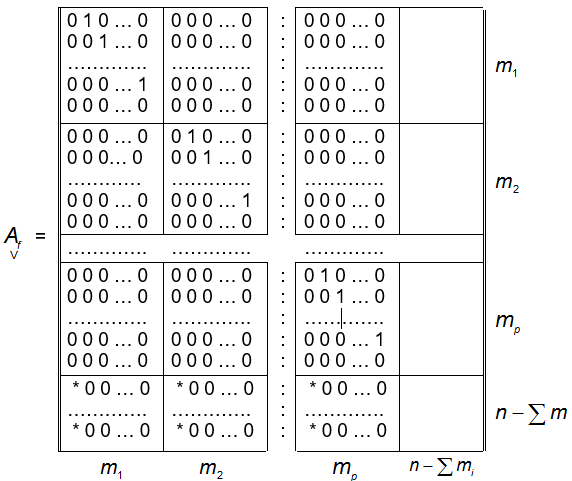
\includegraphics[scale=0.9]{images/Fig3_12_1}
\end{figure}
Эту же матрицу удобнее записать в блочном виде:
\begin{equation}
	\underset{\lor}{A}_f=\begin{bmatrix}
	A_{11} & 0 & \dots & 0 & A_{10}\\
	0 & A_{22} & \dots & 0 & A_{20}\\
	\vdots & \vdots & \vdots & \vdots & \vdots\\
	0 & 0 & \dots & A_{pp} & A_{p0}\\
	A_{01} & A_{02} & \dots & A_{0p} & A_{00}\\
	\end{bmatrix}.
\end{equation}

Разобьём вектор состояния $\vec{x}$ на систему $(p+1)$ частных векторов и обозначим
\begin{equation}
	\vec{x}_f=\begin{bmatrix}
	\vec{z}_1\\\vec{z}_2\\\vdots\vec{z}_p\\\vec{z}_0\\
	\end{bmatrix},
\end{equation}
где $\vec{z}_i$ имеет размерность [$m_i\times1$]. Тогда уравнения (3.10.13) в базисе [$f$] примут вид
\begin{equation*}
	\begin{bmatrix}
	\dot{\vec{z}}_1 \\ \dot{\vec{z}}_2 \\ \vdots \\ \dot{\vec{z}}_p \\ \dot{\vec{z}}_0
	\end{bmatrix}=
	\begin{bmatrix}
	A_{11} & 0 & \dots & 0 & A_{10}\\
	0 & a_{22} & \dots & 0 & A_{20}\\
	\vdots & \vdots & \vdots & \vdots & \vdots\\
	0 & 0 & \dots & A_{pp} & A_{p0}\\
	A_{01} & A_{02} & \dots & A_{0p} & A_{00}
	\end{bmatrix} * 
	\begin{bmatrix}
	\vec{z}_1 \\ \vec{z}_2 \\ \vdots \\ \vec{z}_p \\ \vec{z}_0   
	\end{bmatrix}+
	\begin{bmatrix}
	\vec{\beta}_1 & 0 & \dots & 0\\
	0 & \vec{\beta}_2 & \dots & 0\\
	\vdots & \vdots & \vdots & \vdots\\
	0 & 0 & \dots & \vec{\beta}_p\\
	0 & 0 & \dots & 0\\
	\end{bmatrix} * 
	\begin{bmatrix}
	q_1 \\ q_2 \\ \vdots \\ \vdots \\ q_p
	\end{bmatrix};
\end{equation*}
\begin{equation}
	\begin{bmatrix}
	y_1 \\ y_2 \\ \vdots \\ y_p
	\end{bmatrix}=
	\begin{bmatrix}
	s_1 & 0 & \dots & 0 & 0\\
	0 & s_2 & \dots & 0 & 0\\
	\vdots & \vdots & \vdots & \vdots & \vdots\\
	0 & 0 & \dots & s_p & 0
	\end{bmatrix}*
	\begin{bmatrix}
	\vec{z}_1 \\ \vec{z}_2 \\ \vdots \\ \vec{z}_p \\ \vec{z}_0   
	\end{bmatrix}
\end{equation}
Отсюда следуют уравнения для частных подсистем:
\begin{gather}
\begin{split}
	&\dot{\vec{z}}_i=A_{ii}\vec{z}_i+A_{i0}\vec{z}_0+\vec{\beta}_iq_i;\\
	&y_i=s_i\vec{z}_i, (i=1,2,\dots,p);
\end{split}
\end{gather}
\begin{equation}
\dot{\vec{z}}_0=\sum_{v=1}^{p}A_{0v}\vec{z}_v+A_{00}\vec{z}_0.
\end{equation}
Раскроем систему дифференциальных уравнений для $i$-й подсистемы:
\begin{equation}
\begin{cases}
\dot{z}_{i1}=z_{i2}+a_1^{i10}\vec{z}_0=z_{i2}+g{i1};\\
\dot{z}_{i2}=z_{i3}+g_{i2};\\
\dots\dots\dots\dots\dots\dots\\
\dot{z}_{i,m_i-1}=z_{i,m_i}+g_{i,m_i-1};\\
\dot{z}_{i,m_i}=g_{i,m_i}+q_i;
\end{cases}
\end{equation}
\begin{equation*}
\begin{cases}
y_i=z_{i1},
\end{cases}
\end{equation*}
где $a_1^{i10}$ - первая строка матрицы $A_{i0}$. Такой подсистеме соответствует структурная схема, представленная на рис. 3.13.
\begin{figure}[H]
	\centering
	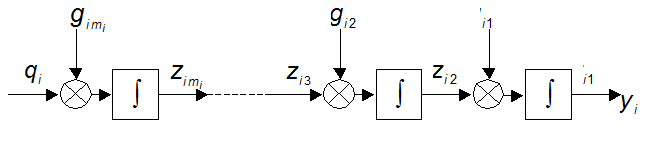
\includegraphics[scale=0.9]{images/Fig3_13}
	\caption{Структурная схема частотной подсистемы}
\end{figure}
Из сопоставления этой схемы со схемой, приведённой на рис. 3.12, следует:
a) $z_{i1}=y_i$; $z_{iv}=y_i^{(v)}$ при $v>1$;
б) $q_{iv}=0$ и $A_{v0}=0$ для $v=1,2,\dots,p$.

Таким образом,  выходы интеграторов частных подсистем, показанных на рис. 3.12, совпали с координатами вектора $\vec{x}$ в базисе [$f$].  Кроме того, все  блочные матрицы $A_{00},A_{10},\dots,A_{p0}$ в (3.10.29)- нулевые. 
	%Проверка работоспособности 
%\chapter{Тестовая зона}
%	$\Delta F_{пр}=K_{пр}\cdot\Delta l_{2} $
%	\begin{equation}
%		Тест \quad русского \quad языка
%	\end{equation}
%	
%	Запишем уравнение центробежного регулятора. Полагая, что сами с
%	
%	\begin{equation}
%	\left(1+K_{зол}K_{2}\cfrac{T_{д}}{T_{д}p+1}\right)\cdot p\Delta l_{сц}=K_{зол}K_{1}\Delta l_{1}
%	\end{equation}
%	
%	\begin{equation}
%	\Delta l_{зол}=K_{1}\cdot\Delta l_{1}-K_{2}\cdot\Delta l_{2}
%	\end{equation}
%	
%	\chapter{Тест нумерации уравнений}
%	\section{первая секция}
%	\begin{equation}\label{key}
%	Первое уравнене
%	\end{equation}
%	\subsection{Подсекция}
%	\begin{equation}\label{key}
%	Уравнение под секции
%	\end{equation}
	
\end{document}